\documentclass{article}
\usepackage{arxiv}

\graphicspath{{../figures/}{figures/}}

\usepackage{tikz}
\usetikzlibrary{positioning,arrows,arrows.meta,calc}
\usepackage{longtable}
\usepackage{booktabs}
\usepackage{tabularx}  % wrapping columns of the numerical-settings table
\usepackage{array}  % >{\raggedright\arraybackslash}p{} columns (Figure~\ref{fig:ast} legend)
\usepackage{natbib}  % provides \citep/\citet; pairs with \bibliographystyle{plainnat}
\usepackage{xurl}  % \url, breakable between any characters (loads url), no hyperlink dependency
\usepackage{placeins}  % \FloatBarrier keeps floats within their section
\usepackage{listings}

% CONVENTION: every numerical result quoted in this paper -- in the prose, the
% figure captions, and the tables -- is drawn from the actual computed data,
% never transcribed or rounded by hand. Headline numbers are emitted as macros
% into generated_values.tex by scripts/make_paper_values.py, and the
% validation tables are generated by scripts/make_validation_tables.py,
% all reading the same figure result caches under results/. To change a number:
% recompute the relevant figure cache, rerun those generators, and rebuild.
% Auto-generated by scripts/make_paper_values.py from the result caches.
% Do not edit by hand; rerun the script after a RECOMPUTE.
\newcommand{\VerifDecayMaxRelErr}{$1.2\times10^{-6}$}
\newcommand{\VerifDecayGradRelErr}{$3.6\times10^{-6}$}
\newcommand{\VerifConsTotalMax}{$8.9\times10^{-16}$}
\newcommand{\VerifADFDMaxRelErr}{$7.8\times10^{-8}$}
\newcommand{\VerifADFDNParams}{five}
\newcommand{\VerifGradTolFloor}{$2.4\times10^{-14}$}
\newcommand{\VerifStiffGradRel}{$7.6\times10^{-6}$}
\newcommand{\VerifStiffRatio}{1000}
\newcommand{\VerifStiffStepRatio}{3}
\newcommand{\VerifPlantFwdRevRel}{$1.0\times10^{-10}$}
\newcommand{\VerifFwdRevRatio}{762}
\newcommand{\VerifADFDWorstName}{$\mu_A$}
\newcommand{\VerifADFDWorstRel}{$2.2\times10^{-7}$}
\newcommand{\VerifADFDHorizon}{120}
\newcommand{\VerifADFDHorizonResid}{$1.1\times10^{-6}$}
\newcommand{\VerifADFDHDefault}{$1.0\times10^{-4}$}
\newcommand{\SteadyNquant}{58}
\newcommand{\SteadyReactorWorstPct}{$3.6\times10^{-3}$}
\newcommand{\SteadyEffWorstPct}{$3.5\times10^{-3}$}
\newcommand{\SteadyTSSWorstPct}{$4.0\times10^{-4}$}
\newcommand{\VerifMassBalCOD}{$2.7\times10^{-11}$}
\newcommand{\VerifMassBalN}{$6.4\times10^{-9}$}
\newcommand{\DynEffSNH}{4.76}
\newcommand{\DynEffSNHRef}{4.76}
\newcommand{\DynEffTN}{15.63}
\newcommand{\DynEffTNRef}{15.57}
\newcommand{\DynEffCOD}{48.29}
\newcommand{\DynEffCODRef}{48.30}
\newcommand{\DynEffTSS}{12.99}
\newcommand{\DynEffTSSRef}{12.99}
\newcommand{\DynEffWorstPct}{0.4}
\newcommand{\DynEQI}{6691}
\newcommand{\DynEQIRef}{6690}
\newcommand{\DynEQIPct}{0.01}
\newcommand{\DynOCI}{16170}
\newcommand{\DynOCIRef}{16148}
\newcommand{\DynOCIPct}{0.14}
\newcommand{\DynSnhNoHoldup}{5.66}
\newcommand{\DynHoldupReldiff}{19}
\newcommand{\DynTankFiveHoldup}{4.3}
\newcommand{\DynTankFiveNoHoldup}{5.2}
\newcommand{\DynHoldupMeanSharePct}{29}
\newcommand{\DynHoldupFlowSharePct}{71}
\newcommand{\DiffParamName}{$\mu_H$}
\newcommand{\DiffTrue}{6.000}
\newcommand{\DiffRecovered}{6.000}
\newcommand{\DiffRecoveredRelErr}{$1.3\times10^{-9}$}
\newcommand{\DiffNobs}{10}
\newcommand{\DiffNsteps}{seven}
\newcommand{\DiffGradFinite}{finite}
\newcommand{\CalNfree}{five}
\newcommand{\CalNbatch}{three}
\newcommand{\CalNobs}{180}
\newcommand{\CalTAerH}{2.4}
\newcommand{\CalTNlimH}{10.8}
\newcommand{\CalTSlimH}{7.2}
\newcommand{\CalNsampAssay}{20}
\newcommand{\CalAerDenseN}{13}
\newcommand{\CalAerDenseMin}{29}
\newcommand{\CalSigSS}{1}
\newcommand{\CalSigSO}{0.1}
\newcommand{\CalSigSNO}{0.2}
\newcommand{\CalNmc}{24}
\newcommand{\CalStartSpread}{0.4}
\newcommand{\CalWorstBias}{1.8}
\newcommand{\CalWorstBiasName}{$\mu_H$}
\newcommand{\CalWorstBiasSE}{0.9}
\newcommand{\CalCoverageRatio}{0.8}
\newcommand{\CalCoverageLo}{0.73}
\newcommand{\CalCoverageHi}{1.07}
\newcommand{\CalSpreadSEPct}{15}
\newcommand{\CalPredCVmu}{9.5}
\newcommand{\CalPredCVetag}{9.3}
\newcommand{\CalPredCVrestLo}{0.3}
\newcommand{\CalPredCVrestHi}{2.6}
\newcommand{\CalEmpCVmu}{10.1}
\newcommand{\CalEmpCVetag}{9.5}
\newcommand{\IdentKappaFull}{$4.5\times10^{4}$}
\newcommand{\IdentKappaAnox}{$>4.5\times10^{15}$}
\newcommand{\IdentCorrFull}{-0.997}
\newcommand{\IdentCorrAnox}{-1.000}
\newcommand{\IdentMuCVanox}{21}
\newcommand{\IdentEtagCVanox}{19}
\newcommand{\IdentProductCVanox}{1}
\newcommand{\IdentNmc}{16}
\newcommand{\IdentProfLoFull}{4.9}
\newcommand{\IdentProfHiFull}{7.1}
\newcommand{\IdentProfLoAnox}{4.8}
\newcommand{\IdentProfGridHi}{10.8}
\newcommand{\IdentMuHTrue}{6.0}
\newcommand{\IdentWeakLoadMu}{$+0.20$}
\newcommand{\IdentWeakLoadEtag}{$-0.98$}
\newcommand{\IdentWeakLoadRatio}{$-0.20$}
\newcommand{\IdentOneMinusEtag}{0.20}
\newcommand{\IdentWeakRelFull}{$2.2\times10^{-5}$}
\newcommand{\IdentWeakRelAnox}{$2.1\times10^{-17}$}
\newcommand{\IdentCrbMuFull}{9.4}
\newcommand{\IdentCrbEtagFull}{9.4}
\newcommand{\IdentAdditivity}{$1.5\times10^{-16}$}
\newcommand{\IdentCrbMuAer}{63}
\newcommand{\IdentCrbBhAer}{1065}
\newcommand{\IdentProdTrue}{4.8}
\newcommand{\DesignDBase}{39.19}
\newcommand{\DesignDOpt}{39.84}
\newcommand{\DesignDetFactor}{1.9}
\newcommand{\DesignNsamp}{20}
\newcommand{\DesignSSBase}{60}
\newcommand{\DesignSSOpt}{200}
\newcommand{\DesignSSLo}{20}
\newcommand{\DesignSSHi}{200}
\newcommand{\DesignSpacingMin}{1.4}
\newcommand{\DesignTaerMin}{144}
\newcommand{\DesignEarlyLo}{4}
\newcommand{\DesignEarlyHi}{11}
\newcommand{\DesignLateLo}{31}
\newcommand{\DesignLateHi}{50}
\newcommand{\DesignCrbMuBase}{9.4}
\newcommand{\DesignCrbMuOpt}{6.8}
\newcommand{\DesignCrbEtagBase}{9.4}
\newcommand{\DesignCrbEtagOpt}{6.8}
\newcommand{\DesignEmpMuOpt}{7.3}
\newcommand{\DesignEmpEtagOpt}{6.7}
\newcommand{\DesignNmc}{24}
\newcommand{\ConsNreactions}{eight}
\newcommand{\ConsResidN}{$-0.17$}
\newcommand{\ConsResidCOD}{$+0.29$}
\newcommand{\ConsNtwoCODperN}{1.71}
\newcommand{\ConsAutoResidCOD}{$-0.006$}
\newcommand{\ConsTol}{$10^{-2}$}
\newcommand{\AdfdRatio}{3.1}
\newcommand{\AdfdProj}{12}
\newcommand{\AdfdFloor}{2.0\times10^{-8}}
\newcommand{\AdfdPlantFloor}{1.4\times10^{-5}}
\newcommand{\AdfdFloorRatio}{718}
\newcommand{\AdfdNrep}{30}
\newcommand{\SteadyPtcIters}{eight}
\newcommand{\SteadyPtcResidual}{$6.1\times10^{-11}$}
\newcommand{\SteadyPtcSpeedupLo}{13}
\newcommand{\SteadyPtcSpeedupHi}{15}
\newcommand{\SteadyFwdSolveMs}{7.1}
\newcommand{\SteadyFwdMatchDays}{164}
\newcommand{\SteadySensRel}{$1.9\times10^{-5}$}
\newcommand{\SteadyFoldSRT}{4.3}
\newcommand{\SteadySRTnominal}{19.1}
\newcommand{\SteadyFoldFailDil}{4.4}
\newcommand{\SteadyNruns}{200}
\newcommand{\SteadyFoldDil}{4.38}
\newcommand{\SteadySensDesign}{0.09}
\newcommand{\SteadySensNearFold}{8}
\newcommand{\SteadySensNearDist}{0.01}
\newcommand{\SteadySensNearPct}{0.2}
\newcommand{\SteadySensGain}{90}
\newcommand{\SteadySensExpStable}{$-0.43$}
\newcommand{\SteadySensExpUnstable}{$-0.58$}
\newcommand{\SteadyFwdHorizon}{300}
\newcommand{\ResidFloor}{10^{-6}}
\newcommand{\PtcTol}{10^{-8}}
\newcommand{\VerifRtol}{10^{-6}}
\newcommand{\VerifAtol}{10^{-9}}
\newcommand{\SIAdjBatchRel}{$9.8\times10^{-10}$}
\newcommand{\SIAdjBatchRtol}{10^{-10}}
\newcommand{\SIAdjBatchCapMin}{10^{-4}}
\newcommand{\SIAdjDigRel}{$2.8\times10^{-7}$}
\newcommand{\SIAdjDigRtol}{10^{-8}}
\newcommand{\SIAdjDigCapMin}{10^{-2}}
\newcommand{\SteadyUnsLam}{2}
\newcommand{\SteadyUnsSacSt}{0.23}
\newcommand{\SteadyUnsSacUns}{4.8}
\newcommand{\SteadyUnsXacSt}{0.76}
\newcommand{\SteadyUnsXacUns}{0.57}
\newcommand{\SteadyUnsSicSt}{0.091}
\newcommand{\SteadyUnsSicUns}{0.026}
\newcommand{\SteadyUnsSacDesSt}{0.09}
\newcommand{\SteadyUnsSacDesUns}{5.2}
\newcommand{\SteadyUnsLamNear}{4}
\newcommand{\SteadyUnsSacNearSt}{1.8}
\newcommand{\SteadyUnsSacNearUns}{3.8}
\newcommand{\SteadyUnsNudgePct}{2}
\newcommand{\SteadyUnsSacWash}{7.3}
\newcommand{\RespNww}{three}
\newcommand{\RespProfileWW}{RWW}
\newcommand{\RespDrErrBest}{6}
\newcommand{\RespDrErrWorst}{30}
\newcommand{\RespDrRtwoLo}{0.77}
\newcommand{\RespDrRtwoHi}{0.84}
\newcommand{\RespMuFitRWW}{3.00}
\newcommand{\RespMuRepRWW}{2.30}
\newcommand{\RespMuFitPCE}{3.66}
\newcommand{\RespMuRepPCE}{3.46}
\newcommand{\RespMuFitRBFE}{2.94}
\newcommand{\RespMuRepRBFE}{2.48}
\newcommand{\RespStRtwo}{0.94}
\newcommand{\RespDrRmseLo}{0.24}
\newcommand{\RespDrRmseHi}{0.29}
\newcommand{\RespStRmseLo}{0.13}
\newcommand{\RespStRmseHi}{0.18}
\newcommand{\RespGuptaOverLo}{2.7}
\newcommand{\RespGuptaOverHi}{5.3}
\newcommand{\RespDrMuStdLo}{0.20}
\newcommand{\RespDrMuStdHi}{0.31}
\newcommand{\RespCodRatioLo}{0.43}
\newcommand{\RespCodRatioHi}{0.61}
\newcommand{\RespProfLoDr}{2.7}
\newcommand{\RespProfHiDr}{3.5}
\newcommand{\RespStMuBound}{0.2}
\newcommand{\RespProfHiSt}{0.25}
\newcommand{\RespProfRepRise}{11}
\newcommand{\RespYH}{0.66}
\newcommand{\RespBH}{0.40}
\newcommand{\RespKSdr}{20}
\newcommand{\RespKSst}{2}
\newcommand{\DigWorstPct}{1.27}
\newcommand{\DigWorstName}{headspace CO$_2$}
\newcommand{\DigMethanePct}{0.62}
\newcommand{\DigNresolvable}{25}
\newcommand{\DigPtcVsFwd}{$8.5\times10^{-9}$}
\newcommand{\DigPH}{7.27}
\newcommand{\DigPHAbsErr}{0.004}
\newcommand{\PerfCompileS}{15.3}
\newcommand{\PerfSolveS}{8.4}
\newcommand{\PerfNstate}{65}
\newcommand{\PerfNparams}{22}
\newcommand{\PerfADFactor}{1.9}
\newcommand{\PerfFDFactor}{23}
\newcommand{\PerfScaleNmin}{4}
\newcommand{\PerfScaleNmax}{256}
\newcommand{\PerfScaleCompileExp}{0.2}
\newcommand{\PerfScaleSolveExp}{1.4}
\newcommand{\PerfNruns}{10}
\newcommand{\PerfScaleNruns}{five}


% Float placement.
\renewcommand{\topfraction}{0.9}
\renewcommand{\bottomfraction}{0.8}
\renewcommand{\textfraction}{0.07}
\renewcommand{\floatpagefraction}{0.75}
\setcounter{topnumber}{3}
\setcounter{bottomnumber}{2}
\setcounter{totalnumber}{5}

% Compact style for inline code and YAML listings.
\lstset{basicstyle=\ttfamily\small, breaklines=true, columns=fullflexible,
        keepspaces=true, showstringspaces=false, frame=single, framesep=4pt,
        rulecolor=\color{gray!40}, xleftmargin=2pt}
\usepackage{xcolor}
% A light YAML style for the example model listing.
\definecolor{yamlkey}{rgb}{0.10,0.28,0.55}
\definecolor{yamlstr}{rgb}{0.50,0.16,0.16}
% Rate-expression token colours (Figure~\ref{fig:ast}); shared by the
% expression legend in panel (a) and the syntax-tree leaves in panel (b).
% Redundant with notation (species wear [ ], functions wear name( )), so
% they still read in grayscale.
\definecolor{rlspec}{HTML}{0B7A75}   % species   (teal)
\definecolor{rlparam}{HTML}{B26A00}  % parameter (amber)
\definecolor{rlfunc}{HTML}{7B3FA0}   % function  (violet)
\definecolor{rlcond}{HTML}{2D5DA8}   % condition (blue)
\newcommand{\rlSpec}[1]{\textcolor{rlspec}{\texttt{#1}}}
\newcommand{\rlParam}[1]{\textcolor{rlparam}{\texttt{#1}}}
\newcommand{\rlFunc}[1]{\textcolor{rlfunc}{\texttt{#1}}}
\newcommand{\rlCond}[1]{\textcolor{rlcond}{\texttt{#1}}}
\newcommand{\rlOp}[1]{\textcolor{black!55}{\texttt{#1}}}
\newcommand{\rlDot}[1]{\tikz[baseline=-0.5ex]\draw[fill=#1,draw=#1] (0,0) circle (2.6pt);}
\lstdefinelanguage{yaml}{
  morekeywords={model, species, conditions, parameters, expressions, reactions},
  keywordstyle=\bfseries\color{yamlkey},
  comment=[l]{\#}, commentstyle=\itshape\color{gray},
  morestring=[b]", stringstyle=\color{yamlstr},
  basicstyle=\ttfamily\footnotesize,
}

\title{A runtime-configurable, automatically differentiable engine for
wastewater treatment process models}

\author{%
  Christopher T. DeGroot\thanks{Corresponding author: \texttt{christopher.degroot@uwo.ca}} \\
  Department of Mechanical and Materials Engineering \\
  Western University, London, ON, Canada \\
}

\date{\today}
\runningheader{A differentiable kinetics engine for wastewater treatment models}

\begin{document}
\maketitle

\begin{abstract}
Wastewater simulators compute solutions, not derivatives, so calibration and sensitivity analysis rely on derivative-free search and finite differences. We present \texttt{aquakin}, an open-source engine in which a plain-text reaction model is reconfigurable at run time and differentiable end to end. Each rate law is compiled from a syntax tree into a differentiable function, never executed as code, and units compose into a plant that is one differentiable program. The engine reproduces the open-loop Benchmark Simulation Model No.~1 to \DynEffWorstPct\,\% in the dry-weather effluent averages, and the benchmark anaerobic digester to \DigWorstPct\,\%. An exact gradient over all \PerfNparams\ plant parameters costs \PerfADFactor\ solves. A differentiable steady-state solver traces the digester through its washout fold. In twin experiments the gradients recover activated-sludge kinetics without bias beyond sampling error, with uncertainties matching the realized spread, and identify and optimize what a design determines. On measured respirograms they discriminate two model structures.
\keywords{differentiable simulation, automatic differentiation, reaction models, activated sludge, BSM1, scientific software}
\end{abstract}

% Highlights (Elsevier: 3-5 bullets, each <= 85 characters incl. spaces).
\section*{Highlights}
\begin{itemize}\setlength\itemsep{1pt}
\item Reaction models are plain-text data, edited and rerun with no code generation
\item Rate laws are parsed to syntax trees and compiled to JAX: safe and differentiable
\item A whole plant is one differentiable program; an exact gradient costs about 2 solves
\item Reproduces open-loop BSM1 and the BSM2 digester; continuation traces its washout
\item Exact gradients drive calibration, identifiability analysis and experimental design
\end{itemize}

% Graphical abstract. Source is the standalone graphical_abstract/graphical_abstract.tex,
% compiled separately to graphical_abstract.pdf (also submitted to EMS as its own file).
\section*{Graphical abstract}
\begin{center}
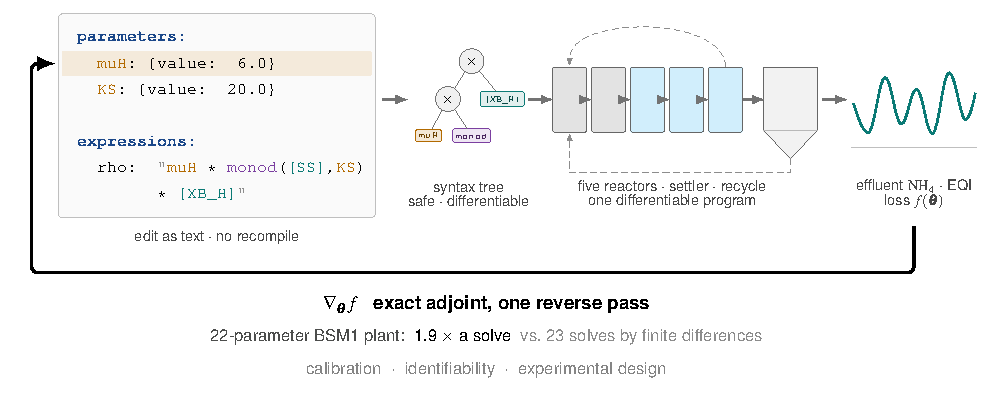
\includegraphics[width=\linewidth]{graphical_abstract/graphical_abstract}
\end{center}

% =========================================================================
\section*{Nomenclature}
\begingroup \small \setlength{\LTleft}{0pt}\setlength{\LTright}{\fill}\setlength{\LTpre}{0pt}\begin{longtable}{@{}ll@{}} \multicolumn{2}{@{}l}{\textit{Abbreviations}}\\ AD & automatic differentiation \\ ADM1 & Anaerobic Digestion Model No. 1 \citep{batstone2002} \\ ASM1 & Activated Sludge Model No. 1 \citep{henze1987, henze2000} \\ ASM3 & Activated Sludge Model No. 3 \citep{henze2000} \\ AST & abstract syntax tree \\ BSM1 & Benchmark Simulation Model No. 1 \citep{copp2002, alex2008} \\ BSM2 & Benchmark Simulation Model No. 2 \citep{jeppsson2007, gernaey2014} \\ COD & chemical oxygen demand \\ DSL & domain-specific language \\ ESDIRK & explicit-first-stage, singly diagonally implicit Runge--Kutta \\ FD & finite difference \\ IFT & implicit function theorem \\ JIT & just-in-time (compilation) \\ JVP & Jacobian--vector product \\ L-BFGS-B & limited-memory BFGS optimizer with bounds \\ ODE & ordinary differential equation \\ OUR & oxygen uptake rate \\ PID & proportional--integral--derivative (step-size controller) \\ PTC & pseudo-transient continuation \\ RHS & right-hand side \\ RMSE & root-mean-square error \\ SER & switched-evolution relaxation \\ YAML & a human-readable data-serialization format \\ \addlinespace[2pt] \multicolumn{2}{@{}l}{\textit{Symbols}}\\ $\mathbf{C}$, $\mathbf{C}_0$ & species concentration vector; its initial value \\ $\mathbf{c}_q$ & content of conserved quantity $q$ per unit of each species \\ $d_i$ & measured value of observation $i$ \\ $\mathbf{F}$ & assembled plant right-hand side, Eq.~\eqref{eq:plant-ode} \\ $\mathbf{F}_{\mathbf{x}}$, $\mathbf{F}_{\alpha}$ & $\partial\mathbf{F}/\partial\mathbf{x}$, $\partial\mathbf{F}/\partial\alpha$ (continuation) \\ $\mathbf{f}$, $\mathbf{f}_u$ & right-hand side of the integrated state $\mathbf{y}$; of unit $u$ \\ $\mathbf{f}_{\boldsymbol{\theta}}$ & parameter derivative $\partial\mathbf{f}/\partial\boldsymbol{\theta}$ \\ $g_i$, $\mathbf{g}_e$ & model prediction of observation $i$; outputs of experiment $e$ \\ $\mathbf{H}$ & Gauss--Newton (Fisher information) matrix $\mathbf{J}_{\mathbf{w}}^{\top}\mathbf{J}_{\mathbf{w}}$ \\ $h$ & hydrogen-ion concentration $[\text{H}^+]$ \\ $\boldsymbol{\mathcal{I}}$ & Fisher information matrix, Eq.~\eqref{eq:fisher} \\ $\mathbf{J}$ & Jacobian of the right-hand side, $\partial\mathbf{f}/\partial\mathbf{y}$ or $\partial\mathbf{F}/\partial\mathbf{x}$ \\ $\mathbf{J}_{\mathbf{w}}$ & residual Jacobian $\partial\mathbf{w}/\partial\boldsymbol{\theta}$ (calibration) \\ $K_a$, $K_b$, $K_w$ & acid and base dissociation constants; water constant \\ $\ell$ & scalar output or loss being differentiated \\ $\mathbf{M}$ & recycle routing matrix \\ $n_s$, $n_r$, $n_p$ & numbers of species, reactions, and parameters \\ $Q$, $\mathbf{Q}$ & stream flow rate; vector of inter-unit flow rates \\ $\mathbf{q}_{\mathrm{ext}}$ & external influent and fixed pumped flows \\ $R(z)$ & stability function of the Runge--Kutta method \\ $\mathbf{r}$ & reaction-rate vector \\ $\mathbf{S}$ & stoichiometry matrix ($n_r\times n_s$) \\ $s$ & number of ESDIRK stages \\ $\mathbf{s}_r$ & stoichiometric coefficients of reaction $r$ (row of $\mathbf{S}$) \\ $T_a$, $T_b$ & total concentration of an acid or base system \\ $t$, $\Delta t$ & time; time step (pseudo-time step in PTC) \\ $\mathbf{u}$ & operating conditions, supplied or state-derived \\ $V$, $\mathbf{V}$ & reactor volume; PTC diagonal scaling matrix \\ $\mathbf{w}$ & weighted residual vector, $w_i=(g_i-d_i)/\sigma_i$, Eq.~\eqref{eq:wls} \\ $\mathbf{x}$, $\mathbf{x}_u$, $\mathbf{x}^\star$ & assembled plant state; state of unit $u$; steady state \\ $\bar{\mathbf{x}}$, $\bar{\mathbf{y}}_n$ & cotangents $\partial\ell/\partial\mathbf{x}^\star$, $\partial\ell/\partial\mathbf{y}_n$ \\ $\mathbf{y}$, $\mathbf{y}_n$ & integrated state ($\mathbf{C}$ or $\mathbf{x}$); its value at step $n$ \\ $z_{\mathrm{cat}}$, $z_{\mathrm{an}}$ & strong-cation and strong-anion charges \\ $\mathbf{Z}_e$, $\mathbf{Z}$ & output sensitivity matrix $\partial\mathbf{g}_e/\partial\boldsymbol{\theta}$ of experiment $e$; \\ & \quad steady-state sensitivity $\partial\mathbf{x}^\star/\partial\boldsymbol{\theta}$ \\ $\mu_H$, $\eta_g$, $Y_H$, \dots & ASM1 and ADM1 variables and parameters, in the notation \\ & \quad of \citet{henze1987} and \citet{batstone2002} \\ $\alpha$, $\alpha_f$ & continuation parameter (feed-flow multiplier); its value at the fold \\ $\gamma$ & diagonal coefficient of the ESDIRK method \\ $\varepsilon$ & scaling floor in $\mathbf{V}$ and $\rho$ \\ $\boldsymbol{\theta}$ & vector of model parameters \\ $\vartheta$ & Arrhenius temperature-correction coefficient \\ $\lambda$ & eigenvalue (of $\mathbf{J}$; $\lambda_k$ of $\boldsymbol{\mathcal{I}}$) \\ $\boldsymbol{\nu}$ & steady-state adjoint, $\mathbf{J}^{\top}\boldsymbol{\nu}=\bar{\mathbf{x}}$ \\ $\rho$ & scaled residual, Eq.~\eqref{eq:scaled-residual} \\ $\boldsymbol{\Sigma}_e$, $\sigma_i$ & measurement-noise covariance; standard deviation \\ $\tau$, $\Delta\tau$ & arclength and its step (continuation) \\ $\Phi$ & charge-balance residual, Eq.~\eqref{eq:charge-balance} \\ $\Phi_D$ & D-criterion $\log\det\boldsymbol{\mathcal{I}}$, Eq.~\eqref{eq:dcrit} \\ $\chi^2$ & weighted least-squares objective, Eq.~\eqref{eq:wls} \\
\end{longtable}
\endgroup

% =========================================================================
\section{Introduction}
\label{sec:intro}

Mechanistic models are central to the design, operation, and analysis of wastewater treatment plants. The activated sludge models used for biological nutrient removal describe a treatment process as a set of chemical species, a rate law for each biological process that transforms them, and the stoichiometry that records how much of each species each process produces or consumes \citep{henze1987, henze2000}. The anaerobic digestion model (ADM1) describes sludge stabilization in the same terms \citep{batstone2002}. The Benchmark Simulation Models assemble both into standard plant layouts for evaluating control and operation \citep{copp2002, alex2008, gernaey2014}. Reaction models of the same form describe chemical treatment as well, including ozonation, advanced oxidation, and disinfection in drinking water. When using software to solve these models, it is important that the software allows the user to easily implement new models to describe the processes of interest and to easily modify existing models as the understanding of the modelled process improves. Another important requirement for many applications is that the software allows the user to obtain the derivative of a model output with respect to the model parameters, which is required for calibration, sensitivity analysis, experimental design, and gradient-based control. The design of a runtime-configurable, differentiable engine for wastewater treatment process models is the subject of this study.

The first requirement, run-time configurability, is a question of how the model is represented and run by the software. The major established wastewater plant simulators, GPS-X \citep{gpsx, gpsxug}, SUMO \citep{sumoslang}, BioWin \citep{biowin}, WEST \citep{vanhooren2003, claeys2006tornado, westmodels}, and SIMBA\# \citep{simba}, all let the user author biokinetic models by entering the species, rate laws, and stoichiometry in a matrix, a spreadsheet, or a dedicated modelling language rather than in the simulator's source code. Each of these is a domain-specific language (DSL), a small notation aimed at one problem area rather than a general-purpose programming language \citep{mernik2005}, though some blur that line by admitting embedded general-purpose code, as SUMO's SumoSlang does with raw C++ blocks. Neighbouring fields describe reaction models the same way. Systems biology exchanges models through the Systems Biology Markup Language, in which each rate law is written as a mathematical formula \citep{hucka2003}; the tools built around it \citep{hoops2006, somogyi2015} mostly interpret that description, while libRoadRunner compiles it just in time to native code when it is loaded \citep{somogyi2015}. Chemical-kinetics solvers such as Cantera read their reaction mechanisms from plain-text files at run time \citep{cantera}. Describing a model in a DSL, apart from the code that solves it, is therefore well established. What distinguishes the tools is what happens to that description once it has been read.

The major wastewater plant simulators parse the customized model description (in whatever form they require) to generate and compile code, which the software then runs as a compiled artifact (to the best of the author's knowledge, according to publicly available documentation). Two consequences follow. A change to the model takes effect only after the description has been regenerated into source code and rebuilt, a step separate from running the simulation. And what executes is a separate program generated from the description rather than the description itself, so anything the software can compute about the running model, beyond its solution, is limited to what that generated program exposes. Run-time configurability is the alternative in which the executable model is built from its data description when the file is loaded, without a separate build step, so that an edit takes effect on the next load. Building it may still involve compilation, as libRoadRunner does by just-in-time compiling SBML models as they are loaded \citep{somogyi2015}. What distinguishes this from code generation is that the compilation is an automatic, in-process step performed when the description is loaded, rather than a separate build. This route has a long history in the domain: the legacy program AQUASIM, still in occasional use, let users define substances, rate laws, and stoichiometry interactively and evaluated them directly \citep{reichert1994}. The open-source Python platform QSDsan \citep{qsdsan} takes the same route today: a process model such as ASM1 is read from a tabular matrix whose rate laws are text, which a symbolic-mathematics library parses and converts to numerical functions when the model is loaded, so that the model can be edited and rerun without a separate build step. PeePyPoo, an open-source package still in development, likewise keeps the model editable as data, assembling it symbolically from tabular process matrices over a Julia symbolic-numeric backend and composing the units into a plant \citep{peepypoo}. Evaluating a user-supplied model directly, however, raises a question of safety. Because a model authored as a portable file is meant to be shared and reused, the file an engine runs need not be one the operator wrote, and it must be treated as untrusted input. Its rate laws are unknown when the software is written, so the software must interpret arbitrary expressions, and the most direct implementation, passing the expression text to a general-purpose evaluator such as Python's \texttt{eval}, runs whatever the text contains and is therefore unsafe \citep{richards2011eval, cwe94}. A symbolic-mathematics parser does not remove the risk by itself: SymPy's expression parser \citep{meurer2017}, used by QSDsan, evaluates the text with Python's \texttt{eval} and is documented as unsafe for unsanitized input \citep{sympyparsing}. A dependable engine must instead interpret user expressions along a restricted path that never executes the raw text as code, and that rejects malformed input with a clear error as the file is loaded rather than failing part-way through a simulation.

The second requirement, differentiability, is the harder of the two to meet. Lack of differentiability does not imply that the established simulators neglect calibration or identifiability. In fact, the well-documented ones provide extensive tooling for both, and this is not new: AQUASIM offered sensitivity analysis, parameter estimation, and identifiability assessment decades ago \citep{reichert1994}. GPS-X carries an automated parameter-estimation optimizer with maximum-likelihood and least-squares objectives, reporting confidence limits, model sensitivity coefficients, and the variance-covariance and correlation matrices from which parameter identifiability is read \citep{gpsx}. WEST provides a suite of virtual experiments: local and global sensitivity analysis, uncertainty analysis by Latin-hypercube sampling, and parameter estimation against measured data \citep{westuserguides}. SUMO exposes sensitivity analysis and parameter optimization through a Python scripting interface that drives the simulator externally \citep{sumodoc}. What none of them exposes is an exact derivative of the model through its solver. A parameter derivative is almost never available in closed form for these models, so it is approximated instead: local sensitivities and the derivatives behind an optimizer's confidence limits are finite differences that perturb one parameter at a time, while global and uncertainty analyses sample the parameter space \citep{gpsx, westuserguides}. Both routes grow more expensive as the number of parameters rises, finite differences add truncation error, and the derivative-free optimizers return no exact curvature, so both calibration and a full identifiability screen become costly and approximate as models grow \citep{vanrolleghem1995, brun2001}. To the author's knowledge, none of the simulators mentioned gives the user that derivative in exact form, whether by reverse-mode automatic differentiation or by an adjoint of the discretized equations. The sensitivities they expose are documented as finite-difference and sampling approximations. Recent work automates the parameter search of calibration rather than changing its nature: \citet{yu2025}, for instance, calibrate an activated-sludge model built in QSDsan using Bayesian optimization and a genetic algorithm, and derive parameter sensitivities from the optimization trials. Such automation removes the manual trial-and-error, but the search stays derivative-free: the number of simulations still grows with the parameter dimension, and parameter importance is inferred from sampled trials rather than computed.

The lack of closed form derivatives does not rule out obtaining exact derivatives. Automatic differentiation computes one from the numerical program itself, by applying the chain rule to the elementary operations the program executes \citep{baydin2018, griewank2008}. It is distinct from finite differencing, which only approximates a derivative and costs one extra model evaluation per parameter, and from symbolic differentiation, which manipulates closed-form expressions and scales poorly. Automatic differentiation has two modes: forward and reverse. Forward mode carries the derivative with respect to a single input through the computation, returning the sensitivity of every output to that input in one pass, and is efficient when the inputs are few. Reverse mode returns the gradient of a single scalar output with respect to all of its inputs in one pass, at a cost essentially independent of the number of inputs. Reverse mode is therefore better-suited to calibration and sensitivity analysis, where one objective depends on many parameters. Applied through a differential equation solver, reverse mode becomes the adjoint method, which yields exact parameter sensitivities of a dynamical model. The methods for computing such derivatives, from forward and reverse-mode differentiation to the discrete and continuous adjoint, are by now well surveyed \citep{chen2018neural, hindmarsh2005, kidger2021on, sapienza2024}. Modern automatic differentiation frameworks make this routine and composable, with just-in-time compilation for speed \citep{jax2018github}. The same machinery underlies scientific-machine-learning approaches that embed learnable components inside the differential equations themselves \citep{rackauckas2020ude}. Differentiable simulation built on this machinery has reshaped several neighbouring fields. Differentiable general circulation models forecast weather and climate at the accuracy of operational systems \citep{kochkov2024neuralgcm}, machine-learning-accelerated solvers cut the cost of computational fluid dynamics \citep{kochkov2021jaxcfd}, differentiable process-based models are now common in the geosciences and hydrology \citep{shen2023diffhydrology}, and in chemistry and systems biology, Catalyst compiles reaction networks written in a symbolic domain-specific language into the differentiable solvers of the Julia scientific-machine-learning ecosystem \citep{loman2023}. In each case the value of differentiability has been realized through what the gradients enable for that field, demonstrated on its own benchmark problems.

Wastewater modelling has largely not followed. In water and wastewater, machine learning has been coupled with the governing equations mainly through physics-informed neural networks, which train a neural network to satisfy those equations rather than differentiating the mechanistic model itself. Valuable as such hybrids are for data-driven inference, they learn a surrogate of the process and inherit well-documented training difficulties on the stiff, multi-scale, and networked systems that plant-wide wastewater models present \citep{dibella2026}. The mechanistic reaction models themselves, despite an established benchmark family in the Benchmark Simulation Models \citep{copp2002, alex2008, gernaey2014}, are not ordinarily available in differentiable form. A general automatic differentiation framework, a library such as JAX that differentiates any program written with its array operations \citep{jax2018github}, could supply one, but only once the model has been expressed as such a program. For a wastewater model, that means either writing its governing equations against the framework directly, and rewriting them for every change of model, which surrenders the run-time reconfigurability the domain needs, or building a translator from the model description into the framework, together with the assembly of the plant, its recycle loops and the composition of its units, into one differentiable program. Exact differentiation and run-time reconfigurability are each available; what is missing in wastewater applications is a single engine in which they hold together.

Holding the two together is the specific obstacle. A model reconfigured at run time must evaluate rate laws that are unknown when the software is written, and that same evaluation must be safe, differentiable, and fast at once. The obvious routes each secure some of these at the cost of another: compiling the rate laws into code gives up run-time configurability; evaluating their text directly gives up safety and yields no derivatives; and generating and compiling code for each model reintroduces a separate build step and executes a generated program rather than the description. Meeting all of them together requires a different construction.

This paper presents \texttt{aquakin}, an open-source Python engine built for that combination. Its contribution is the union of two capabilities that already exist in isolation: automatic differentiation of stiff systems and run-time editing of a biokinetic model. It is a reaction model reconfigured as data that remains safe, differentiable end to end, and composable into a plant. Its specific contributions are the following.
\begin{enumerate}
\item A plain-text reaction-model format and a validating schema that declare the species, the operating conditions, the parameters, the rate laws, and the stoichiometry of a model at run time, in terms close to those a modeller would write by hand (Sections~\ref{sec:methods-twolayer}--\ref{sec:methods-format}).
\item A safe, differentiable rate-expression evaluator. Each rate law is parsed by a recursive-descent parser into an abstract syntax tree, and that tree is compiled through JAX into a just-in-time, differentiable function. The text is never executed as code and no per-model source code is generated, so the evaluator is safe and introspectable while remaining differentiable and fast (Sections~\ref{sec:methods-parser}--\ref{sec:methods-eval}).
\item A plant-wide composition that assembles reacting and non-reacting unit operations into a single flowsheet, resolves the recycle loops directly, and integrates the whole plant under one solver, so the end-to-end differentiability of a single unit extends to the assembled plant (Section~\ref{sec:methods-plant}).
\item Verification against a closed-form solution, against a stoichiometric conservation audit, and against finite-difference gradients, and reproduction of the open-loop BSM1 benchmark at steady state and across the dry-weather dynamic envelope (Sections~\ref{sec:results-verification}--\ref{sec:results-dynamic}). A demonstration that the exact gradients make multi-parameter calibration a direct computation, recovering activated-sludge kinetics without bias from noisy batch assays, and that the same Fisher information reads the practical identifiability of an experimental design, at a gradient cost independent of the number of parameters (Section~\ref{sec:results-diff}).
\item A differentiable steady-state solver. The plant steady state is found by pseudo-transient continuation as an algebraic root rather than by long forward integration, its parameter sensitivities follow from the implicit function theorem, and a pseudo-arclength continuation deliberately traverses and locates the saddle-node fold at which a methanogenic operating state ceases to exist, the anaerobic-digester washout (Sections~\ref{sec:methods-steady} and \ref{sec:results-steadysolver}).
\end{enumerate}

Table~\ref{tab:landscape} places \texttt{aquakin} among the existing tool classes; it is the only one to combine all five capabilities.

\begin{table}[htbp]
\centering
\caption{Where \texttt{aquakin} sits among existing tool classes for wastewater process modelling. Only \texttt{aquakin} combines all five capabilities; the contribution is the combination, not any single column.}
\label{tab:landscape}
\small
\begin{tabular}{lccccc}
\toprule
Tool class & Edit at & Exact gradient & Cost indep. & Recycle-coupled & Open \\
 & run time$^{*}$ & through solver & of $N_p$ & plant & source \\
\midrule
Commercial wastewater simulators$^{a}$       & no  & no  & no  & yes & no  \\
QSDsan$^{b}$                                  & yes & no  & no  & yes & yes \\
Differentiable-ODE / adjoint libraries$^{c}$ & no  & yes & yes & no  & yes \\
\texttt{aquakin} (this work)                  & yes & yes & yes & yes & yes \\
\bottomrule
\end{tabular}
\\[3pt]
{\footnotesize $N_p$ is the number of calibrated parameters. $^{*}$Model structure edited and rerun without a code-generation and compilation step.
$^{a}$GPS-X, SUMO, BioWin, WEST, SIMBA\#; model edits take effect only after a code-generation and compilation step, local sensitivities are obtained by finite differencing, one parameter at a time, and global ones by sampling.
$^{b}$Rate laws are parsed with a symbolic-mathematics library and integrated numerically; sensitivity and uncertainty analysis are sampling-based.
$^{c}$e.g.\ Diffrax and SUNDIALS/CVODES; these expose exact adjoint gradients but differentiate equations fixed in code, with no reconfigurable model or plant composition.}
\end{table}

The payoff follows from the premise. Once a reconfigurable model is differentiable from end to end, calibration, identifiability analysis, experimental design, and gradient-based control become direct computations at a gradient cost independent of the number of parameters. The engine is not tied to one chemistry: because a model is supplied as data, the same machinery reads any reaction model of this form, the schemes of water chemistry included. We make the case on the field's own benchmark family, the activated-sludge process and the anaerobic digester, where the same gradients reproduce the established benchmark results, recover reaction kinetics from noisy data, reveal what a given experiment can identify, and locate the operating boundary at which an anaerobic digester washes out.

% =========================================================================
\section{Software architecture}
\label{sec:methods}

\texttt{aquakin} is designed so that a reaction model supplied as data becomes a differentiable numerical function. Section~\ref{sec:methods-model} describes how a model file is represented and turned into a differentiable rate function, from the two-layer design through the rate-expression parser, the differentiable evaluation of the resulting syntax trees, and the safety guarantees and the stoichiometric conservation audit. Section~\ref{sec:methods-assembly} covers the simulation of a single reactor and of a full plant assembled from connected units, solved both in time and at steady state. Section~\ref{sec:methods-ad} covers the gradients, the sensitivities, and the Fisher-information read-out of identifiability. Sections~\ref{sec:methods-bsm1config}--\ref{sec:methods-calibstudy} give the configurations of the case studies used in this paper, the BSM1 plant, the anaerobic digester, and the batch and respirometric calibration studies, and Section~\ref{sec:methods-repro} the steps to reproduce the results.

\subsection{Representing and evaluating a reaction model}
\label{sec:methods-model}

\subsubsection{Two-layer data model}
\label{sec:methods-twolayer}

A model is loaded in two stages that separate the load-time concerns of validation and clear error reporting from the run-time concern of fast, differentiable evaluation (Figure~\ref{fig:framework}). The first stage parses the file and validates it against a declarative schema built with Pydantic \citep{Colvin_Pydantic_Validation_2026}. The format itself is described in Section~\ref{sec:methods-format}. The schema fixes the type and admissible range of every field and the structure of the model as a whole. It requires that a species default concentration be non-negative, that a parameter value lie within its stated bounds, that species and reaction names be unique, and that every species named in a stoichiometry be a declared species. A key the schema does not recognize, such as a mistyped field name, is rejected rather than silently ignored. A malformed model is reported at load time, before any computation runs, with a message that locates the problem: a schema error names the offending field, and a rate-law error names the reaction and the offending identifier. The first stage yields a validated specification, a set of typed objects that carry no numerical machinery.

A compilation step then turns that specification into the compiled model, the object on which the rest of the engine operates. It holds the stoichiometry matrix $\mathbf{S}$ and the vector of model parameters $\boldsymbol{\theta}$, at their default values, as JAX arrays, and the parsed rate laws as a single vectorized rate function that evaluates all of them at once, sharing repeated subexpressions, and is just-in-time compiled together with the solver that calls it (Sections~\ref{sec:methods-parser}--\ref{sec:methods-eval}). That function also depends on the operating conditions $\mathbf{u}$, such as temperature, that the rate laws draw on from outside the kinetics, the third input to the solve in Figure~\ref{fig:framework} alongside the state and the parameters. It retains no dependency on the schema layer. The integrators and the gradient computations operate only on the compiled model. The validation machinery is therefore absent from these repeatedly evaluated functions, and the cost of validation is paid once, at load time, rather than on every evaluation.

\begin{figure}[htbp]
  \centering
  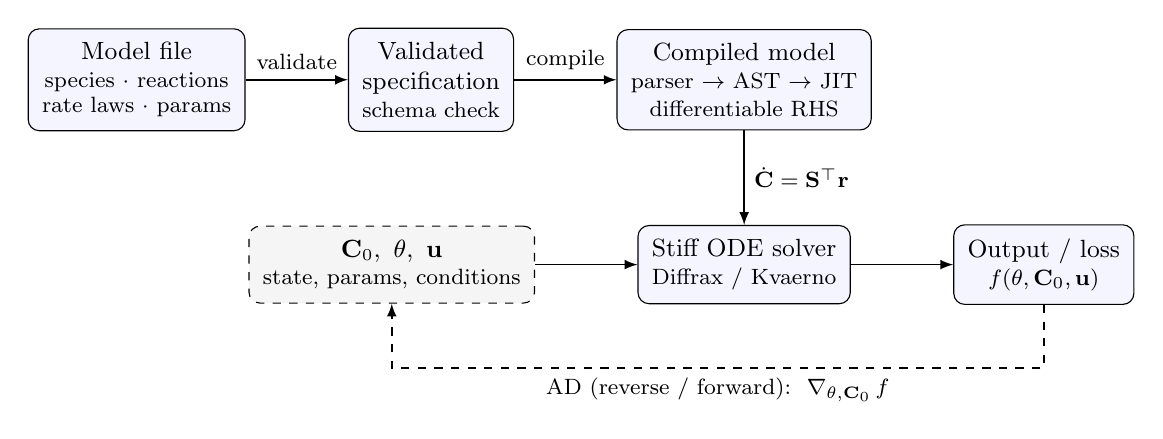
\begin{tikzpicture}[
      node distance=7mm and 13mm,
      box/.style={draw, rounded corners, align=center, inner sep=5pt,
                  font=\small, fill=blue!4},
      io/.style={draw, dashed, rounded corners, align=center, inner sep=5pt,
                 font=\small, fill=gray!8},
      arr/.style={->, >=latex, semithick},
    ]
    \node[box] (yaml) {Model file\\[-1pt]{\footnotesize species $\cdot$ reactions}\\[-2pt]{\footnotesize rate laws $\cdot$ params}};
    \node[box, right=of yaml] (spec) {Validated\\specification\\[-1pt]{\footnotesize schema check}};
    \node[box, right=of spec] (comp) {Compiled model\\[-1pt]{\footnotesize parser $\to$ AST $\to$ JIT}\\[-1pt]{\footnotesize differentiable RHS}};
    \node[box, below=12mm of comp] (solv) {Stiff ODE solver\\[-1pt]{\footnotesize Diffrax / Kvaerno}};
    \node[box, right=of solv] (out) {Output / loss\\[-1pt]{\footnotesize $f(\boldsymbol{\theta},\mathbf{C}_0,\mathbf{u})$}};
    \node[io, left=of solv] (inp) {$\mathbf{C}_0,\ \boldsymbol{\theta},\ \mathbf{u}$\\[-1pt]{\footnotesize state, params, conditions}};

    \draw[arr] (yaml) -- (spec) node[midway, above, font=\footnotesize] {validate};
    \draw[arr] (spec) -- (comp) node[midway, above, font=\footnotesize] {compile};
    \draw[arr] (comp) -- (solv) node[midway, right, font=\footnotesize] {$\dot{\mathbf{C}}=\mathbf{S}^\top \mathbf{r}$};
    \draw[arr] (inp) -- (solv);
    \draw[arr] (solv) -- (out);
    \draw[arr, dashed] (out.south) -- ++(0,-8mm) -| (inp.south)
      node[pos=0.25, below, font=\footnotesize] {AD (reverse / forward):\ \ $\nabla_{\boldsymbol{\theta},\mathbf{C}_0}\, f$};
  \end{tikzpicture}
  \caption{The \texttt{aquakin} pipeline for a single reacting unit. A model
  declaration is validated against a schema and compiled into the right-hand side
  \(\dot{\mathbf{C}}=\mathbf{S}^\top \mathbf{r}(\mathbf{C},\boldsymbol{\theta},\mathbf{u})\).
  Each rate law is parsed into an abstract syntax tree and emitted as a
  just-in-time compiled, differentiable callable. Given an initial state,
  parameters, and conditions, a stiff solver returns the trajectory and any scalar
  output \(f\). Because the whole path is differentiable, automatic
  differentiation returns \(\nabla_{\boldsymbol{\theta},\mathbf{C}_0} f\) in either
  mode. The plant-wide model of Section~\ref{sec:methods-plant} composes many such
  units into one differentiable system integrated by a single solver.}
  \label{fig:framework}
\end{figure}

\subsubsection{The reaction-model format}
\label{sec:methods-format}

A model is declared in a plain-text YAML file, the format of which was designed so that a modeller can read the file, recognize the model, and edit a rate law or add a species by editing text rather than code. The file is a DSL of the same kind as the simulators' model descriptions and the Systems Biology Markup Language (Section~\ref{sec:intro}). Like the latter, it expresses each rate law as a mathematical formula over the declared species, parameters, and conditions, and like a Cantera mechanism, it is read at run time with no intermediate code generation. Listing~\ref{lst:asm1compact} shows one complete process of the Activated Sludge Model No.~1 in this form (the aerobic growth of heterotrophs). The file is organized into blocks. The \texttt{model} block carries the metadata: the model's name, version, description, and literature references. The \texttt{species} block lists the state variables and their units. The \texttt{conditions} block, not shown in the excerpt, declares the operating conditions supplied from outside the kinetics, such as temperature. The \texttt{parameters} block lists the rate and stoichiometric parameters with their default values, and optionally the bounds and the transform that a calibration uses to keep each parameter physical (e.g., a positive-log transform for a rate constant and a logit transform for a yield), and optionally a temperature-correction factor and a Gaussian prior. The \texttt{expressions} block gives a name to a rate law so that a reaction, or another expression, can reference it. The \texttt{reactions} block declares each reaction as a rate and a set of stoichiometric coefficients, one per species the reaction touches.

\lstinputlisting[language=yaml, float=tp, caption={A simplified excerpt of the shipped \texttt{asm1.yaml}: one process, the aerobic heterotrophic growth of the Activated Sludge Model No.~1, with the version, references, descriptions, parameter units, default concentrations, temperature corrections and priors of the full file left out. A concentration is written in brackets inside a rate law, and the yield-dependent stoichiometric coefficients are written as expressions in the yield \texttt{Y\_H} rather than as pre-multiplied numbers. Elisions (\texttt{\#~...}) mark the further species, parameters, and processes of the complete file.}, label={lst:asm1compact}]{asm1_compact.yaml}

Two key features of the rate and stoichiometry are visible in the listing. First, within a rate law, a species concentration is written in brackets, so \texttt{[SS]} is the substrate concentration and the Monod term \texttt{[SS]/(KS~+~[SS])} reads as it would on paper. Second, a stoichiometric coefficient may itself be an algebraic expression of the parameters rather than a number. In the aerobic-growth process the substrate and oxygen coefficients are written as \texttt{-1/Y\_H} and \texttt{-(1-Y\_H)/Y\_H}, the yield-dependent forms of the activated sludge models, rather than as pre-multiplied constants. Because the coefficient is the expression, calibrating the yield \texttt{Y\_H} adjusts every coefficient that depends on it, in this reaction and in the anoxic-growth reaction, with no further bookkeeping.

The format also supports inheritance, so a model may extend another: the entries it declares override the base's field by field or are added by name, and a \texttt{remove} block drops named species, conditions, reactions, parameters or expressions. It also supports declaring the elemental and COD content of each species, so that the stoichiometry can be audited for conservation (Section~\ref{sec:methods-safety}). All models used in this study ship with the library as YAML model declarations.

\subsubsection{The rate-expression language and parser}
\label{sec:methods-parser}

The rate laws are the part of the model that must be evaluated, and they are not known until the file is read. Three requirements shape how \texttt{aquakin} evaluates them. First, a model file is data, not trusted code, so evaluating its rate laws by executing them as Python would run arbitrary text from the file, carrying a security risk. Second, the rate must be differentiable, so that exact parameter gradients are available through it. Finally, the model must be open to inspection, so that names can be checked, the stoichiometry can be audited for conservation (Section~\ref{sec:methods-safety}), and repeated subexpressions can be shared. The engine meets all three by evaluating each rate law through a small expression language that is parsed into a syntax tree, rather than by executing the text as code or by generating and compiling per-model source, neither of which satisfies these requirements cleanly.

The expression language is a small, fixed vocabulary that is used to define expressions in the model file (Figure~\ref{fig:ast}a). Its operands are the quantities of the model, which include: species concentrations, written in brackets, e.g.\ as \texttt{[SS]}; parameters, written in plain text, e.g.\ \texttt{muH}; the names of the expressions defined in the \texttt{expressions} block, also written in plain text; operating conditions such as temperature or pH, written in braces, e.g.\ \texttt{\{T\}}; and numeric constants, written as integer or floating point numbers. These combine through the arithmetic operators \texttt{+ - * /}, exponentiation \texttt{**}, and parentheses, and through a set of named functions that capture the kinetic forms common to environmental models. The named functions include the Monod saturation term \texttt{monod(X,K)}$\,=X/(K+X)$ and its inhibition and ratio variants, the Arrhenius rate factor \texttt{arrhenius(A,Ea)}$\,=A\,e^{-E_a/(RT)}$, which reads the temperature condition, and switching and inhibition functions of a state-derived pH. The Monod term may equivalently be written out as the arithmetic \texttt{[SS]/(KS + [SS])}, as in Listing~\ref{lst:asm1compact}, so the named functions are a convenience over the same operations rather than a separate mechanism. No name or operation outside this vocabulary is admissible.

A recursive-descent parser reads each rate law string once, at load time, and produces an abstract syntax tree, which is a representation of the expression as a tree whose branch points are the operators and named functions and whose leaves are the quantities they act on, i.e.\ the species, parameters, conditions, named expressions, and numeric constants (Figure~\ref{fig:ast}b). Compiling the tree, which also happens when the model is loaded, resolves every species, parameter, condition, and named-expression reference against the declared model, so a reference to an undeclared name is reported at load time with the offending name rather than producing a wrong result at run time. The tree is the structure that the next section evaluates in forming the model equations. 

\begin{figure}[tp]
  \centering
  \begin{minipage}[t]{0.53\linewidth}
    \centering
    \textbf{(a) Expression language}\par\medskip
    \raggedright
    A rate law combines a small, fixed set of building blocks. The
    aerobic-growth rate, as written in the model file, is\par\smallskip
    \hspace*{0.5em}\rlParam{muH} \rlOp{*} \rlSpec{[SS]} \rlOp{/} \rlOp{(}\rlParam{KS} \rlOp{+} \rlSpec{[SS]}\rlOp{)} \rlOp{*} \rlSpec{[XB\_H]}\par\smallskip
    and the recurring saturation pattern
    \rlSpec{[SS]}\rlOp{/}\rlOp{(}\rlParam{KS}\rlOp{+}\rlSpec{[SS]}\rlOp{)}
    may be written with the named function \rlFunc{monod}:\par\smallskip
    \hspace*{0.5em}\rlParam{muH} \rlOp{*} \rlFunc{monod}\rlOp{(}\rlSpec{[SS]}\rlOp{,} \rlParam{KS}\rlOp{)} \rlOp{*} \rlSpec{[XB\_H]}\par\medskip
    \setlength{\tabcolsep}{4pt}
    \begin{tabular}{@{}l >{\raggedright\arraybackslash}p{0.52\linewidth}@{}}
      \rlDot{rlspec}~\rlSpec{[species]}   & a state concentration, \mbox{from $\mathbf{C}$}\\[2pt]
      \rlDot{rlparam}~\rlParam{parameter} & a rate or yield constant, \mbox{from $\boldsymbol{\theta}$}\\[2pt]
      \rlDot{rlcond}~\rlCond{\{condition\}} & an operating condition, \mbox{from $\mathbf{u}$}\\[2pt]
      \rlDot{rlfunc}~\rlFunc{function}     & a kinetic form (\rlFunc{monod}, \rlFunc{arrhenius}, \dots)\\[2pt]
      \rlOp{+~-~*~/~**}                   & operators and grouping\\
    \end{tabular}
  \end{minipage}\hfill
  \begin{minipage}[t]{0.43\linewidth}
    \centering
    \textbf{(b) Syntax tree}\par\medskip
    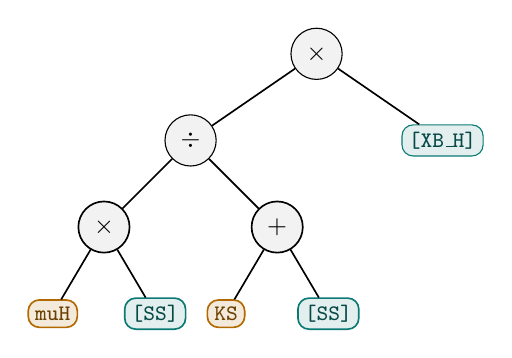
\begin{tikzpicture}[
        font=\small,
        op/.style={draw, circle, inner sep=1.2pt, fill=black!5, minimum size=6.5mm},
        spleaf/.style={draw=rlspec, rounded corners, inner sep=2.5pt, fill=rlspec!12,
                       font=\ttfamily\footnotesize, text=rlspec!60!black},
        parleaf/.style={draw=rlparam, rounded corners, inner sep=2.5pt, fill=rlparam!14,
                        font=\ttfamily\footnotesize, text=rlparam!60!black},
        level 1/.style={sibling distance=32mm, level distance=11mm},
        level 2/.style={sibling distance=22mm, level distance=11mm},
        level 3/.style={sibling distance=13mm, level distance=11mm},
        edge from parent/.style={draw, semithick},
      ]
      \node[op]{$\times$}
        child {node[op]{$\div$}
          child {node[op]{$\times$}
            child {node[parleaf]{muH}}
            child {node[spleaf]{[SS]}}}
          child {node[op]{$+$}
            child {node[parleaf]{KS}}
            child {node[spleaf]{[SS]}}}}
        child {node[spleaf]{[XB\_H]}};
    \end{tikzpicture}\par\medskip
    {\footnotesize\raggedright The parser turns the string into this
    tree. Operators are interior nodes; the coloured leaves are the
    operands of panel~(a). Each leaf is one array lookup and each
    interior node one differentiable operation.\par}
  \end{minipage}
  \caption{The rate-expression language and its syntax tree.
  (a)~A rate law is composed from a small, fixed vocabulary: operands
  (a species concentration in brackets, a parameter, a condition, or a
  constant), the arithmetic operators, and named kinetic functions such
  as \texttt{monod}. The colours distinguish the operand and function
  kinds and are reused on the tree in panel~(b). A recurring pattern
  such as the Monod term may be written explicitly or through its named
  function; nothing outside the vocabulary is admissible, which is what
  makes evaluating a model file safe. (b)~The parser turns the rate-law
  string into an abstract syntax tree, here the substrate-limited
  aerobic-growth rate \texttt{muH * [SS] / (KS + [SS]) * [XB\_H]} (the
  oxygen Monod term of the full rate is analogous and omitted for
  clarity). Operators are interior nodes and the operands are the
  leaves. Evaluating the rate is a single upward traversal, in which
  each leaf is an array lookup and each interior node one differentiable
  JAX operation (Section~\ref{sec:methods-eval}); a quantity that
  recurs, such as \texttt{[SS]}, is computed once and shared.}
  \label{fig:ast}
\end{figure}

\subsubsection{Differentiable evaluation of the syntax trees}
\label{sec:methods-eval}

The abstract syntax tree is the bridge between the human-readable rate law and a differentiable numerical function. The engine evaluates it in JAX \citep{jax2018github}, a numerical-computing framework that provides automatic differentiation and just-in-time compilation. Each node maps to an elementary JAX operation. A leaf in the tree maps to an array lookup or a constant, while an interior node maps to the corresponding arithmetic or library call. Walking the tree from its leaves up to its root, applying each node's operation to the values returned by its children, therefore emits a JAX computation that evaluates the rate expression. Because every elementary operation in that computation has a known derivative, the rate is differentiable with respect to the species concentrations, the parameters, and the conditions. This walk runs only once, when the rate function is first built, and JAX then compiles the computation it produces ``just in time''. Neither the Python interpreter nor the walk over the tree recurs on a solver step, so both are absent from the inner integration loop. 

Subexpressions that recur across the reactions of a model are identified and evaluated once, and the reactions of the whole model are compiled together into a single vectorized kernel. Therefore, every instance of a given operation across all the reactions is evaluated as one batched array operation, rather than as a separate scalar operation per reaction. The size of the compiled kernel therefore grows with the number of distinct operation types and the depth of the expressions, not with the number of reactions, which is what keeps the one-time compilation nearly flat in the model size (Section~\ref{sec:results-performance}). This batching shares work across the reactions rather than recomputing common terms. This changes only how the rates are evaluated, not their values.  The kernel has been verified to return, bit for bit, the same rate vector that a separate evaluation of each reaction would.

All compiled rate functions share one signature. They map a concentration vector \(\mathbf{C}\in\mathbb{R}^{n_s}\), a flat parameter vector \(\boldsymbol{\theta}\in\mathbb{R}^{n_p}\), and the operating conditions \(\mathbf{u}\) to the reaction-rate vector \(\mathbf{r}\in\mathbb{R}^{n_r}\). The stoichiometry matrix \(\mathbf{S}\in\mathbb{R}^{n_r\times n_s}\), the analogue of the Petersen matrix of the activated sludge models, turns this rate vector into the reaction term of the species mass balance, so under reaction alone the concentrations change as
\begin{equation}
  \dot{\mathbf{C}} = \mathbf{S}^\top \mathbf{r}(\mathbf{C}, \boldsymbol{\theta}, \mathbf{u}).
  \label{eq:massbalance}
\end{equation}
This reaction term is the complete balance of a closed unit and the source term to which the continuously-fed reactors of Section~\ref{sec:methods-reactor} add transport. The rate parameters enter through \(\boldsymbol{\theta}\) and are never written into the compiled function, so the model output is differentiable with respect to every parameter. This is the prerequisite for the gradient-based calibration and sensitivity analysis of Section~\ref{sec:results-diff}.

\subsubsection{State-derived conditions: pH from charge balance}
\label{sec:methods-conditions}

A condition may be computed from the instantaneous state at each function evaluation, rather than supplied from outside, and is then passed to the rate expressions in $\mathbf{u}$ like any other condition. Because such a state-derived condition is a differentiable function of the state, the gradient still flows through it. The pH of the anaerobic-digestion model is one such quantity, since it is not a state, but is fixed by electroneutrality. Writing \(h=[\text{H}^+]\), so that \(\text{pH}=-\log_{10} h\), the hydrogen-ion concentration \(h\) is the root of the charge-balance residual
\begin{equation}
  \Phi(h,\mathbf{C}) = h - \frac{K_w}{h} + z_{\mathrm{cat}} - z_{\mathrm{an}}
    + \sum_{b} T_b\,\frac{h}{h+K_b}
    - \sum_{a} T_a\,\frac{K_a}{h+K_a} = 0,
  \label{eq:charge-balance}
\end{equation}
where \(K_w\) is the water constant, \(z_{\mathrm{cat}}\) and \(z_{\mathrm{an}}\) the strong-ion charges, and each acid/base total \(T_x\) (the carbonate, ammonia, and volatile-fatty-acid systems) is read from the state \(\mathbf{C}\) and speciated into its charged fraction at the temperature-corrected constant \(K_x\). The engine solves Eq.~\eqref{eq:charge-balance} for \(h\) at each evaluation by a safeguarded Newton iteration held inside a physical bracket, and supplies the pH to the pH-dependent switching and inhibition functions (Section~\ref{sec:methods-parser}). 

Because the pH is a differentiable function of the state and parameters through this root, its sensitivity to the parameters is obtained by the implicit function theorem at the converged root rather than by differentiating the Newton iteration. It is one of the engine's implicit-solve derivatives and is derived, alongside the steady-state sensitivity, in Section~\ref{sec:methods-ad}. This machinery is exercised and verified in the anaerobic-digester model of Sections~\ref{sec:methods-digesterconfig} and~\ref{sec:results-steadysolver}.

\subsubsection{Safety, introspection, and conservation}
\label{sec:methods-safety}

Because the rate laws are parsed into a syntax tree rather than executed as code, the engine never runs arbitrary text. Only the declared species, parameters, conditions, and the fixed set of named kinetic functions can appear in a valid expression, and any other name is rejected at load time. The syntax tree is also open to inspection, so the engine can report the structure of a rate law, and the declared stoichiometry supports a conservation audit. Since every reaction is declared as explicit stoichiometry, and the model may declare the content of a conserved quantity such as COD or an element per unit of each species (the bundled models ship such a composition table), the conservation of that quantity is a property of the stoichiometry alone. Writing \(\mathbf{c}_q\) for the content of a conserved quantity \(q\) per unit of each species, a reaction with stoichiometry \(\mathbf{s}_r\) conserves \(q\) when \(\mathbf{s}_r\!\cdot\!\mathbf{c}_q=0\). The audit is independent of the kinetics: stoichiometric coefficients that depend on parameters, such as \(1/Y_H\), are evaluated at given parameter values, and the residual \(\mathbf{s}_r\!\cdot\!\mathbf{c}_q\) of every reaction and quantity is reported above a tolerance (\ConsTol\ by default). It is run on request, before any simulation, so a stoichiometric error is caught at the source, and it reports rather than rejects, since some imbalances are intended, such as nitrogen leaving a reaction as dinitrogen gas that the model does not carry as a species.

\subsection{Simulating reactors and plants}
\label{sec:methods-assembly}

The engine simulates a single reactor and a full plant with the same rate machinery and the same solvers. The single reactor is the base case (Section~\ref{sec:methods-reactor}). A plant is a collection of reacting and non-reacting units connected by streams, with material recycled from downstream units back to upstream ones (Section~\ref{sec:methods-plant}). Once assembled, either is advanced in time by the stiff solver of Section~\ref{sec:methods-integration} or driven to its steady state by the solver of Section~\ref{sec:methods-steady}.

\subsubsection{Single reactors}
\label{sec:methods-reactor}

The base case is a single well-mixed reactor. A closed batch reactor exchanges no material with its surroundings and evolves under the reaction term alone, the mass balance of Eq.~\eqref{eq:massbalance}. Adding an influent and an effluent stream gives a continuously-fed reactor. For a reactor of volume \(V\) fed by inlet streams \(\{(Q_m,\mathbf{C}_m)\}\) and drawn off at an outlet flow \(Q^{\mathrm{out}}\), the concentrations follow the continuous-flow mass balance
\begin{equation}
  \dot{\mathbf{C}}
  = \frac{1}{V}\!\left(\sum_m Q_m \mathbf{C}_m - Q^{\mathrm{out}}\,\mathbf{C}\right)
    + \mathbf{S}^\top \mathbf{r}(\mathbf{C}, \boldsymbol{\theta}, \mathbf{u}).
  \label{eq:cstr}
\end{equation}
This continuous-flow balance is the building block from which a plant is assembled.

\subsubsection{Plant-wide composition}
\label{sec:methods-plant}

A plant is a set of units connected by streams, where material can flow upstream to downstream and can also be recycled from downstream units back to upstream ones. The plant module composes reacting units with non-reacting unit operations into a flowsheet. Each stream carries a flow rate \(Q\) and a concentration vector \(\mathbf{C}\). Each unit declares its internal state \(\mathbf{x}_u\), its input and output ports, a function that computes its outlet streams from its inlet streams and state, and the right-hand side \(\mathbf{f}_u\) that governs the evolution of that state, \(\dot{\mathbf{x}}_u = \mathbf{f}_u\). For a reacting well-mixed unit \(u\), that \(\mathbf{f}_u\) is the continuous-flow balance of Eq.~\eqref{eq:cstr} in the unit's own state \(\mathbf{x}_u\), with the inlet streams routed to it by the wiring. A non-reacting unit drops the reaction term and keeps the transport and separation terms. A unit's state need not be a single well-mixed concentration vector. For example, the ten-layer secondary settler of the validation plant (Section~\ref{sec:methods-bsm1config}) is one unit whose state \(\mathbf{x}_u\) stacks the concentrations of all ten layers, with \(\mathbf{f}_u\) the matching stack of per-layer balances. In general \(\mathbf{x}_u\) may hold any number of internal variables, so long as \(\mathbf{f}_u\) supplies the matching right-hand side.

The plant assembles every unit's state into one flat vector \(\mathbf{x}=(\mathbf{x}_1,\dots,\mathbf{x}_U)\), whose right-hand side collects the per-unit balances,
\begin{equation}
  \dot{\mathbf{x}} = \mathbf{F}(\mathbf{x}, \boldsymbol{\theta}, t),
  \qquad
  \mathbf{F} = \big(\mathbf{f}_1, \dots, \mathbf{f}_U\big),
  \label{eq:plant-ode}
\end{equation}
where each unit right-hand side \(\mathbf{f}_u\) is that unit's balance and depends on its own state and on the inlet streams routed to it by the wiring. The assembled plant is therefore one combined system in the same form as a single reactor. Because that right-hand side is one differentiable function, the end-to-end differentiability of a single unit extends to the plant, and a gradient of a plant-level output flows across every unit and every connection.

The flow network has recycle loops, so the inter-unit flows cannot be read off in a single downstream pass but must be solved for. The flow part of the network is linear and independent of the concentrations. Each unit's throughflow is the external feed routed to it plus the recycled fractions of the other units' flows, so the flow vector \(\mathbf{Q}\) is defined in terms of itself, a fixed-point relation. Because that relation is linear in \(\mathbf{Q}\) plus a constant feed term, the fixed point is affine and solves in closed form. Collecting the flows in \(\mathbf{Q}\),
\begin{equation}
  \mathbf{Q} = \mathbf{M}\mathbf{Q} + \mathbf{q}_{\mathrm{ext}}
  \quad\Longrightarrow\quad
  \mathbf{Q} = (\mathbf{I}-\mathbf{M})^{-1}\mathbf{q}_{\mathrm{ext}},
  \label{eq:flow-fixedpoint}
\end{equation}
where \(\mathbf{M}\) is the recycle routing matrix, its entries being the fraction of each stream sent from one unit to another, and \(\mathbf{q}_{\mathrm{ext}}\) is the external influent and the fixed pumped setpoints. The product \(\mathbf{M}\mathbf{Q}\) is the recirculated flow, so the relation reads that each flow is what returns to it plus what enters from outside, and the inversion on the right gives it in closed form. The plant computes this inverse directly rather than by fixed-point iteration. Iteration converges slowly when the loop gain, the fraction of a stream that returns to a unit after passing around the recycle loops, approaches one, as it can in a flowsheet whose splitters return fixed fractions of their inflow. The direct solve keeps the flows exact regardless. (In BSM1 the internal recycle and the return sludge are fixed pump setpoints, so its flows follow directly.) The recycled concentrations pose a fixed point of the same kind, since the composition returned to a unit depends on the outlets downstream of it. The plant resolves it by an adaptive iteration started from the exact solution of its linear part and run to a relative tolerance of \(10^{-8}\), and differentiates the converged result by the implicit function theorem, so the gradient is exact and does not depend on the number of passes. It needs \(\mathbf{I}-\mathbf{M}\) non-singular, which holds whenever the routing is sub-conservative (i.e., each unit passes on no more flow than it receives, so a recycle returns only a fraction of a stream and never amplifies it). The spectral radius of \(\mathbf{M}\), its largest eigenvalue in magnitude, is then below one, which guarantees the inverse \((\mathbf{I}-\mathbf{M})^{-1}\) exists, as it does for any physical flowsheet. This closed-form solve assumes only that the routing is independent of the concentrations. 

When the influent or a scheduled pump setpoint varies over a run, the routing matrix \(\mathbf{M}\) is unaffected, so it is formed once per solve and each integration step redoes only the cheap linear solve of Eq.~\eqref{eq:flow-fixedpoint} for the resampled feed \(\mathbf{q}_{\mathrm{ext}}(t)\), which is exact and requires no iteration. A control law that sets a flow from a measured concentration, such as a solids-based return-sludge rate, is the case that couples the two. In such cases, the setpoint then depends on the state, so \(\mathbf{M}\) is re-formed from the current state at each integration step rather than reused, with the concentration read before the flows are resolved so the affine solve stays exact at that instant. The plant's state is the unit states rather than the inter-unit streams, so a stream such as the settler effluent is reconstructed on demand by re-running the output computation at a saved state, which matches the wiring exactly.

\subsubsection{Dynamic integration}
\label{sec:methods-integration}

The assembled system, a single reacting unit or a whole plant alike, is integrated with Diffrax \citep{kidger2021on}, a JAX-native differential equation library, using an implicit method of the ``explicit-first-stage, singly diagonally implicit Runge--Kutta'' (ESDIRK) family, the Kvaerno methods, with adaptive step-size control. The stiff kinetics of wastewater reactor models call for an implicit method. ESDIRK methods advance the state over a step \(\Delta t\) through a short sequence of stages. Being singly diagonally implicit, each stage solves a nonlinear system for its own stage value, and every stage of a step shares the same operator \(\mathbf{I}-\gamma\,\Delta t\,\mathbf{J}\), where \(\gamma\) is a single constant on the method's diagonal and \(\mathbf{J}\) is the Jacobian of the right-hand side, so one Jacobian factorization is reused across the whole step. The first stage is explicit (the E of ESDIRK) so a step of \(s\) stages costs \(s-1\) implicit solves. The tolerances and per-experiment settings are collected in Section~\ref{si:settings}.

The reason to pay for an implicit method is how it treats the fast reaction modes. Linearizing the rates about the current state, each eigenmode of \(\mathbf{J}\) with eigenvalue \(\lambda\) is carried across a step by multiplication with the method's stability function \(R(\lambda\,\Delta t)\), a rational function fixed by the method's coefficients. A fast reaction mode near quasi-equilibrium has a large negative \(\lambda\), a relaxation time far shorter than \(\Delta t\), so \(\lambda\,\Delta t\) is large and negative. An explicit method amplifies such a mode unless \(\Delta t\) is cut below that fast timescale, which is the step-size restriction that makes stiff systems expensive to solve using such methods. The ESDIRK method is instead L-stable, a property with two parts, stated here in the argument \(z=\lambda\,\Delta t\). First, \(\lvert R(z)\rvert\le 1\) everywhere in the left half-plane \(\operatorname{Re}(z)\le 0\), which is exactly the region where the exact mode decays, so no decaying mode is amplified at any step size (this first part alone is A-stability). Second, \(R(z)\to 0\) as \(\operatorname{Re}(z)\to-\infty\), so the fastest modes, those with the most negative \(z\), are driven almost to zero within a single step. The mechanism is through the implicit stage solve itself, which applies \((\mathbf{I}-\gamma\,\Delta t\,\mathbf{J})^{-1}\) and contracts the eigendirections of \(\mathbf{J}\) that have a large negative eigenvalue, so within one step the fast modes settle to the quasi-equilibrium values the slow variables dictate, just as they do in the exact dynamics. The step is then sized by the accuracy wanted on the slow, resolved dynamics rather than by the stability limit of the fast modes, which is what lets the solver take large steps on a stiff system.

The integration uses 64-bit floating-point arithmetic, which the library enables globally on import. Holding those fast modes near their quasi-equilibrium repeatedly forms small net differences between large, nearly cancelling reaction terms. Subtracting nearly equal quantities loses accurate digits to rounding \citep{goldberg1991}, so single precision is not sufficient. 

An optional clamp protects the saturation kinetics from a transiently negative state by evaluating the rates on the non-negative part \(\max(C,0)\) of the concentration vector, a standard activated-sludge convention. Where every concentration is positive, the clamp is the identity and does not enter the gradient. At an exact zero boundary it gives a one-sided subgradient rather than the smooth derivative. In the solves whose gradients are reported here this happens only for the dissolved oxygen held near zero in the anoxic tanks and anoxic assays. There the reported gradients still agree with finite differences (Section~\ref{sec:results-verification-fd}), which are subject to the same clamp, so the subgradient does not corrupt the reported results.

\subsubsection{Steady-state solution}
\label{sec:methods-steady}

Several analyses solve for the steady state of a reactor or plant, rather than following a transient integration. The steady state is the root of the assembled right-hand side,
\begin{equation}
  \mathbf{F}(\mathbf{x}, \boldsymbol{\theta}) = \mathbf{0}.
  \label{eq:steady}
\end{equation}
Forward integration to the attractor does reach the solution, but it is slow, because the slowest pools, a long-retention digester or the slow autotrophic biomass, equilibrate only over long horizons. A plain Newton root-find is fast near the solution but, from a poor start, stalls at a local minimum of \(\lVert\mathbf{F}\rVert\) or overshoots into nonphysical states. The engine bridges the two with pseudo-transient continuation \citep{kelley1998, pattison2014}, which advances the damped-Newton step
\begin{equation}
  \left(\tfrac{1}{\Delta t}\mathbf{V} - \mathbf{J}\right)\Delta\mathbf{x} = \mathbf{F}(\mathbf{x}),
  \qquad \mathbf{x} \leftarrow \mathbf{x} + \Delta\mathbf{x},
  \qquad \mathbf{J} = \frac{\partial\mathbf{F}}{\partial\mathbf{x}},
  \label{eq:ptc}
\end{equation}
with the Jacobian \(\mathbf{J}\) formed exactly by automatic differentiation of the right-hand side. The pseudo-time term \(\mathbf{V}/\Delta t\) is a regularization that ensures stability.  At a small pseudo-timestep \(\Delta t\) the step is a stable backward-Euler move along the physical transient, globally convergent like time-stepping. As the residual falls, the timestep is grown by switched-evolution relaxation (SER), \(\Delta t \leftarrow \Delta t\,\rho_{\mathrm{old}}/\rho_{\mathrm{new}}\) in the scaled residual \(\rho\) of Eq.~\eqref{eq:scaled-residual} below, with the ratio limited to \([0.2,\,10]\) per step, until the term vanishes and Eq.~\eqref{eq:ptc} becomes Newton's method with its quadratic terminal convergence. The diagonal scaling \(\mathbf{V}=\operatorname{diag}(\max(\lvert\mathbf{x}\rvert,\varepsilon))\) gives each state a magnitude-consistent pseudo-time, which matters where plant states span orders of magnitude, from a dissolved oxygen of order unity to a biomass of order thousands. Each step is also safeguarded. Its length is first capped so that no currently positive state is driven through zero (a fraction-to-boundary rule), and a backtracking line search then shortens it until its residual is within a fixed factor of the best residual reached so far. A step that cannot be brought within that bound is rejected: the iterate is held and \(\Delta t\) is cut by a factor of ten toward the backward-Euler limit. A cold start therefore cannot run away to a nonphysical state, while a converging run is unaffected. Convergence is measured by the scaled residual
\begin{equation}
  \rho(\mathbf{x}) = \max_i \frac{\lvert F_i(\mathbf{x},\boldsymbol{\theta})\rvert}{\max(\lvert x_i\rvert,\varepsilon)},
  \label{eq:scaled-residual}
\end{equation}
the largest rate of change of any state relative to its own magnitude, with the same scaling as \(\mathbf{V}\) and \(\varepsilon=\ResidFloor\) so that states near zero do not dominate. With \(\mathbf{F}\) in units per day, \(\rho\) is the fractional change per day of the state that is still changing fastest relative to its own magnitude. The iteration stops once \(\rho\) falls below a tolerance, and the same \(\rho\) is used throughout the paper to judge whether a forward-integrated state has reached steady state.

The root find breaks down where the Jacobian \(\partial\mathbf{F}/\partial\mathbf{x}\) is singular, which the operating branch approaches as a control parameter drives it toward a stability boundary. Let \(\alpha\) be that scalar parameter and hold the rest of \(\boldsymbol{\theta}\) fixed. The operating branch is the curve of solutions of Eq.~\eqref{eq:steady} as \(\alpha\) varies. Stepping \(\alpha\) and re-solving for \(\mathbf{x}\), i.e.\ natural-parameter continuation, fails at a fold, where the branch turns back on \(\alpha\) and \(\partial\mathbf{F}/\partial\mathbf{x}\) is singular. The solver instead parameterizes the branch by arclength \(\tau\) and appends a pseudo-arclength constraint \citep{allgower2003},
\begin{equation}
  \dot{\mathbf{x}}_0^{\top}(\mathbf{x}-\mathbf{x}_0) + \dot{\alpha}_0\,(\alpha-\alpha_0) = \Delta\tau,
  \label{eq:arclength}
\end{equation}
in which \((\dot{\mathbf{x}}_0,\dot{\alpha}_0)\), the unit-length solution of \(\mathbf{F}_{\mathbf{x}}\dot{\mathbf{x}}+\mathbf{F}_{\alpha}\dot{\alpha}=\mathbf{0}\), is the tangent to the branch at the previous point \((\mathbf{x}_0,\alpha_0)\), \(\Delta\tau\) is the step, and \(\mathbf{F}_{\mathbf{x}}=\partial\mathbf{F}/\partial\mathbf{x}\), \(\mathbf{F}_{\alpha}=\partial\mathbf{F}/\partial\alpha\). This tangent is the Euler predictor for the next point, and a Newton corrector refines it on the augmented system of Eqs.~\eqref{eq:steady} and \eqref{eq:arclength}. The continuation works in scaled states, each divided by its magnitude at the known solution (floored at \(10^{-3}\)), so that large and small states contribute comparably to the arclength. The augmented system's Jacobian
\begin{equation}
  \begin{bmatrix} \mathbf{F}_{\mathbf{x}} & \mathbf{F}_{\alpha} \\[3pt] \dot{\mathbf{x}}_0^{\top} & \dot{\alpha}_0 \end{bmatrix}
  \label{eq:bordered}
\end{equation}
stays non-singular at a simple fold, where \(\mathbf{F}_{\mathbf{x}}\) drops rank but the bordering row and column restore it. The continuation therefore reaches operating points a direct solve cannot and, carrying \(\dot{\alpha}\) through zero at the turning point, traverses the fold, traces the otherwise-unreachable unstable branch, and locates the saddle-node itself, the bifurcation past which no operating steady state exists \citep{seydel2010}. The fold is marked by \(\dot{\alpha}=0\), where the loading is momentarily stationary along the branch and the natural-parameter sensitivity \(\partial\mathbf{x}/\partial\alpha=-\mathbf{F}_{\mathbf{x}}^{-1}\mathbf{F}_{\alpha}\) diverges as \(\mathbf{F}_{\mathbf{x}}\) loses rank; the continuation reports the fold location, to within its step along the branch, and the diverging sensitivity pinpoints it.

\subsection{Gradients and sensitivities}
\label{sec:methods-ad}

\subsubsection{Modes, exactness, and cost}

Because the map from the parameters and initial conditions to any model output is a composition of elementary operations with known derivatives, that map is differentiable from end to end. Reverse-mode automatic differentiation returns the gradient of a scalar output with respect to all of its inputs in a single pass, at a cost essentially independent of the number of inputs. This is the key differentiating feature of \texttt{aquakin}: the gradient of a batch- or plant-level loss with respect to the whole parameter vector is one reverse pass, at a constant cost (a small multiple of a single solve) regardless of how many parameters it is taken against (Section~\ref{sec:results-performance}). In contrast, a finite-difference gradient costs a full solve per parameter. Calibration and sensitivity analysis are therefore direct gradient computations that do not scale with the parameter count, the regime in which derivative-free and finite-difference methods become expensive.

Throughout, an exact gradient means the exact gradient of the discrete program the solver executes, as distinct from a finite-difference approximation. It carries the discretization error of the solve but introduces none of its own, so its disagreement with a known analytic derivative is set by the solver tolerance and falls to floating-point precision as the tolerance is tightened, as will be shown. On the other hand, a finite difference carries a step-size error that is truncation-limited at large steps and solver-noise-limited at small ones.

\subsubsection{Differentiating the solve}

How the reverse pass is taken through the solve depends on the computation, and the choice bears on the exactness. For a non-stiff or short transient the engine differentiates the adaptive integrator directly, by a checkpointed reverse pass that reconstructs the forward states and returns the exact gradient of the discrete trajectory. Over a stiff solve taken with large implicit steps, as in the coupled plant and the batch calibration, differentiating through the solve accumulates the reverse-mode sensitivities of the large stage values of the fast modes and can overflow the floating-point range even where the primal solution is accurate, unless the step size is limited. This is a known difficulty in differentiating stiff systems \citep{kim2021stiff}. The engine instead forms the reverse-mode gradient with a discrete adjoint, the established construction for implicit Runge--Kutta methods used in stiff chemical-kinetics and sensitivity solvers \citep{sandu2003, zhang2014}. 

The forward pass is an ordinary adaptive implicit solve, and the backward pass is the analytic transposed solve of the same implicit steps. The object carried backward is the \emph{cotangent} of the state, which is defined as the gradient of the scalar output \(\ell\) (a calibration loss or any reported scalar) with respect to the state. The integrated state \(\mathbf{y}\) represents either a unit's \(\mathbf{C}\) or the assembled plant \(\mathbf{x}\), while its right-hand side is \(\mathbf{f}\). The parameter derivative is \(\mathbf{f}_{\boldsymbol{\theta}}=\partial\mathbf{f}/\partial\boldsymbol{\theta}\) and \(\bar{\mathbf{y}}_n=\partial\ell/\partial\mathbf{y}_n\) is the cotangent of the state at step \(n\). The construction is simplest to show on one implicit-Euler step, \(\mathbf{y}_{n+1}=\mathbf{y}_n+\Delta t\,\mathbf{f}(\mathbf{y}_{n+1},\boldsymbol{\theta})\); the high-order ESDIRK method the solver actually uses follows the same pattern. For the step \(n\), already taken on the forward pass, one backward step turns the later cotangent \(\bar{\mathbf{y}}_{n+1}\) into the earlier one \(\bar{\mathbf{y}}_n\) through a single transposed linear solve,
\begin{equation}
  (\mathbf{I}-\Delta t\,\mathbf{J}^{\top})\,\bar{\mathbf{y}}_{n}=\bar{\mathbf{y}}_{n+1},
  \qquad
  \mathbf{J}=\frac{\partial\mathbf{f}}{\partial\mathbf{y}}\bigg|_{\mathbf{y}_{n+1}},
  \label{eq:discrete-adjoint}
\end{equation}
and adds one term \(\Delta t\,\mathbf{f}_{\boldsymbol{\theta}}^{\top}\bar{\mathbf{y}}_n\) to the parameter gradient. Taking the steps from the last to the first assembles that gradient as a sum over the whole trajectory,
\begin{equation}
  \frac{\partial\ell}{\partial\boldsymbol{\theta}}=\sum_{n}\Delta t\,\mathbf{f}_{\boldsymbol{\theta}}^{\top}\bar{\mathbf{y}}_{n},
  \label{eq:adjoint-grad}
\end{equation}
in which \(\mathbf{f}_{\boldsymbol{\theta}}=\partial\mathbf{f}/\partial\boldsymbol{\theta}\), like \(\mathbf{J}\), is evaluated at that step's stored state \(\mathbf{y}_{n+1}\).

The step's two operations draw on different machinery. The model derivatives \(\mathbf{J}=\partial\mathbf{f}/\partial\mathbf{y}\) and \(\mathbf{f}_{\boldsymbol{\theta}}=\partial\mathbf{f}/\partial\boldsymbol{\theta}\) are supplied by automatic differentiation of the rate function at \(\mathbf{y}_{n+1}\), and each term \(\Delta t\,\mathbf{f}_{\boldsymbol{\theta}}^{\top}\bar{\mathbf{y}}_n\) is the matching vector--Jacobian product. Reverse mode automatic differentiation propagates \(\bar{\mathbf{y}}_n\) back through \(\mathbf{f}\) to produce \(\mathbf{f}_{\boldsymbol{\theta}}^{\top}\bar{\mathbf{y}}_n\) in a single pass, delivering the Jacobian's action on \(\bar{\mathbf{y}}_n\) (which is just one vector) rather than actually forming the full matrix \(\mathbf{f}_{\boldsymbol{\theta}}\). The cotangent \(\bar{\mathbf{y}}_n\) is the one quantity obtained by solving a linear system.  Its operator \(\mathbf{I}-\Delta t\,\mathbf{J}^{\top}\) is the transpose of the matrix \(\mathbf{I}-\Delta t\,\mathbf{J}\) of the forward step's implicit solve. The backward step re-forms \(\mathbf{J}\) at the saved state by automatic differentiation and solves the transposed system directly, so the backward pass needs only the saved states, not the forward solver's factorisations. Only the recurrence itself, the transposed solve and the sum, is written by hand in the code; everything model-specific comes from automatic differentiation. The backward pass runs from the last step to the first, with each observation's contribution to \(\ell\) added to the state cotangent at the step where that observation falls. Because the stiff dissipative dynamics make \(\mathbf{I}-\Delta t\,\mathbf{J}^{\top}\) a contraction, the cotangent stays bounded and no step size limit is needed. The result is still the exact gradient of the discrete trajectory but with the assurance that it will not overflow. The high-order version used in practice replaces the single implicit stage with the transposed-stage recurrence of the \(s\)-stage ESDIRK method the reactors use, reconstructing the stage values from the solver's saved increments; the full construction is given in Section~\ref{si:discrete-adjoint}. This version of the adjoint is the reverse-mode path used for the calibration and the plant.

The same sensitivities are available using forward mode automatic differentiation, the counterpart to the reverse-mode discrete adjoint. Rather than differentiate through the solve, the engine integrates the sensitivity \(\partial\mathbf{y}/\partial\boldsymbol{\theta}\) alongside the state, as the augmented variational system
\begin{equation}
  \dot{\mathbf{y}}=\mathbf{f}(\mathbf{y},\boldsymbol{\theta}),
  \qquad
  \frac{\mathrm{d}}{\mathrm{d}t}\frac{\partial\mathbf{y}}{\partial\boldsymbol{\theta}}
  =\frac{\partial\mathbf{f}}{\partial\mathbf{y}}\,\frac{\partial\mathbf{y}}{\partial\boldsymbol{\theta}}
  +\frac{\partial\mathbf{f}}{\partial\boldsymbol{\theta}},
  \label{eq:variational}
\end{equation}
advanced as one system \([\mathbf{y};\,\partial\mathbf{y}/\partial\boldsymbol{\theta}]\) under a single adaptive step controller whose error norm bounds the sensitivity as well as the state. The state keeps its usual error control, and the step is tightened further only where the sensitivity itself is stiff, so no step-size limitation has to be imposed by hand for the sensitivity solve \citep{hindmarsh2005}. The augmented system carries one sensitivity column per parameter, so although it is a single integration its cost grows with the number of parameters; forward mode therefore suits few parameters or many outputs, while reverse mode suits the many-parameter calibration. Forward and reverse are independent algorithms for the same derivative and agree to the solver tolerance, which is one of the verification checks shown in Section~\ref{sec:results-verification-fd} (there the forward-mode side is taken through the solve rather than by the variational system).

The remaining solves are algebraic rather than time-stepped and are obtained by the implicit function theorem at the converged root. The steady-state root find (Section~\ref{sec:methods-steady}) and the pH charge balance (Section~\ref{sec:methods-conditions}) fall into this category. 

For the steady state, \(\mathbf{x}^\star\) is the root of \(\mathbf{F}(\mathbf{x}^\star,\boldsymbol{\theta})=\mathbf{0}\) (Eq.~\eqref{eq:steady}). Differentiating that identity at the root gives the parameter sensitivity
\begin{equation}
  \frac{\partial\mathbf{x}^\star}{\partial\boldsymbol{\theta}}
  = -\left(\frac{\partial\mathbf{F}}{\partial\mathbf{x}}\right)^{-1}\frac{\partial\mathbf{F}}{\partial\boldsymbol{\theta}}.
  \label{eq:ift}
\end{equation}
Reverse mode evaluates the corresponding gradient without ever forming this matrix. For a scalar output \(\ell\), let \(\bar{\mathbf{x}}=\partial\ell/\partial\mathbf{x}^\star\) be the gradient of that output with respect to the state, obtained directly by one reverse-mode pass through the output function. With \(\mathbf{J}=\partial\mathbf{F}/\partial\mathbf{x}\), contracting Eq.~\eqref{eq:ift} from the left with \(\bar{\mathbf{x}}\) gives
\begin{equation}
  \frac{\partial\ell}{\partial\boldsymbol{\theta}}
  = -\bar{\mathbf{x}}^{\top}\mathbf{J}^{-1}\frac{\partial\mathbf{F}}{\partial\boldsymbol{\theta}}
  = -\boldsymbol{\nu}^{\top}\frac{\partial\mathbf{F}}{\partial\boldsymbol{\theta}},
  \label{eq:ift-adjoint}
\end{equation}
where the adjoint \(\boldsymbol{\nu}\) is defined by \(\boldsymbol{\nu}^{\top}=\bar{\mathbf{x}}^{\top}\mathbf{J}^{-1}\). The adjoint can be equivalently defined by the transposed system \(\mathbf{J}^{\top}\boldsymbol{\nu}=\bar{\mathbf{x}}\), which is actually used to solve for \(\boldsymbol{\nu}\), which avoids inverting \(\mathbf{J}\). \(\mathbf{J}\) is formed afresh at the converged root by automatic differentiation, so the gradient depends only on the root and not on how the pseudo-transient iteration reached it (Section~\ref{sec:methods-steady}). One such solve yields the whole gradient, so the steady-state sensitivity is exact and, like the transient adjoint, independent of the number of parameters. The full derivation is given in Section~\ref{si:steady-adjoint}.

The pH of the anaerobic-digestion model is differentiated the same way. It is not a state but a state-derived condition (Section~\ref{sec:methods-conditions}), fixed by the charge-balance root \(\Phi(h,\mathbf{C},\boldsymbol{\theta})=0\) of Eq.~\eqref{eq:charge-balance}. Differentiating that identity along the solution gives its sensitivity by the same theorem,
\begin{equation}
  \frac{\partial\Phi}{\partial h}\,\frac{\partial h}{\partial\boldsymbol{\theta}}
    + \frac{\partial\Phi}{\partial\boldsymbol{\theta}} = 0
    \quad\Longrightarrow\quad
  \frac{\partial h}{\partial\boldsymbol{\theta}}
   = -\left(\frac{\partial\Phi}{\partial h}\right)^{-1}\frac{\partial\Phi}{\partial\boldsymbol{\theta}}.
  \label{eq:ph-ift}
\end{equation}
This is a single scalar solve because \(h\) is scalar, with \(\partial\Phi/\partial h>0\) since \(\Phi\) is strictly increasing in \(h\) (the same monotonicity that makes the charge-balance root unique). A rate that depends on pH therefore stays exactly differentiable, and the gradient flows through the condition as through any other elementary operation, at no extra solve.

\subsubsection{Calibration, Fisher information, and identifiability}

The same differentiation gives not only the gradient of a scalar loss but the Jacobian of a vector of outputs or residuals with respect to the parameters. These are the same quantities that calibration and experimental design rest on and are built from that Jacobian with no additional solves. A local sensitivity of a set of outputs to the parameters is read from this Jacobian in either mode, forward when the outputs outnumber the parameters and reverse when the parameters outnumber the outputs. This is reported, for an output \(g\) and a parameter \(\theta\), as an elasticity \((\partial g/\partial\theta)(\theta/g)\). The elasticity is dimensionless so that it is comparable across parameters and outputs of different units and magnitudes (Section~\ref{sec:results-diff}).

Calibration fits a model by minimizing a weighted least-squares objective. With \(g_i(\boldsymbol{\theta})\) the model prediction of observation \(i\), \(d_i\) its measured value, and \(\sigma_i\) its measurement standard deviation, the weighted residual is \(w_i=(g_i-d_i)/\sigma_i\) and the objective is
\begin{equation}
  \chi^2(\boldsymbol{\theta})=\tfrac12\lVert\mathbf{w}(\boldsymbol{\theta})\rVert^2=\tfrac12\sum_i w_i(\boldsymbol{\theta})^2 ,
  \label{eq:wls}
\end{equation}
the negative log-likelihood of the parameters under independent Gaussian measurement noise. A Gaussian prior adds a quadratic term, giving the maximum-a-posteriori objective the calibration routine uses below.

The residual Jacobian \(\mathbf{J}_{\mathbf{w}}=\partial\mathbf{w}/\partial\boldsymbol{\theta}\) is supplied by automatic differentiation. The exact Hessian of \(\chi^2\) is \(\mathbf{J}_{\mathbf{w}}^{\top}\mathbf{J}_{\mathbf{w}}+\sum_i w_i\,\partial^2 w_i/\partial\boldsymbol{\theta}^2\); near a good fit the residuals are small, so the residual-weighted second term is dropped and the engine forms the Gauss--Newton, or Fisher information, matrix \(\mathbf{H}=\mathbf{J}_{\mathbf{w}}^{\top}\mathbf{J}_{\mathbf{w}}\) at the cost of that one Jacobian. The Jacobian is taken in the unconstrained coordinates in which the fit runs (described below), so \(\mathbf{H}\) and its inverse are in those coordinates, and the standard deviations of the physical parameters follow by the chain rule. When Gaussian priors are used, they enter as additional residual rows, so \(\mathbf{H}\) then also carries the prior information. Its inverse \(\mathbf{H}^{-1}\), where the design is non-degenerate, is the Laplace covariance of the estimate (equivalently the inverse Fisher information, the Cram\'er--Rao floor on the parameter variances) so every fit carries a full parameter uncertainty with no further solves; a parameter on an exactly null direction of \(\mathbf{H}\), one the data do not constrain at all, is reported with an infinite standard deviation. The diagonal of \(\mathbf{H}^{-1}\) gives the marginal variance, and hence a standard error, of each parameter. The normalized off-diagonals of \(\mathbf{H}^{-1}\) are the parameter correlations, and a correlation approaching \(\pm1\) means the data fix only a combination of two parameters, not each alone \citep{brun2001, brun2002}.

The eigenstructure of \(\mathbf{H}\) is a direct read indicator of practical identifiability. A large eigenvalue marks a well-determined parameter combination, while a near-zero eigenvalue marks a sloppy one that the data barely constrain, along which the covariance \(\mathbf{H}^{-1}\) diverges. The condition number measures the spread between the stiff and sloppy directions, a structure common to these models \citep{gutenkunst2007}. Because \(\mathbf{H}=\mathbf{J}_{\mathbf{w}}^{\top}\mathbf{J}_{\mathbf{w}}\) is built from the residual Jacobian alone, which depends on the measurement design (e.g., the sampling times, inputs, and weights) and on the assumed parameters, but not on the measured values, it can be assembled before any data are collected, which makes it the basis of the optimal experimental design described below. Where the quadratic approximation behind \(\mathbf{H}\) is in doubt near a degeneracy, a profile likelihood provides a check that does not rely on it. It fixes one parameter across a grid of values and re-optimizes the others at each value, and the shape of the resulting curve separates a structurally non-identifiable parameter from one that is merely poorly determined \citep{raue2009}. Where this profile agrees with the Gaussian covariance, it confirms that approximation.

Evaluated at assumed parameter values rather than at a fitted optimum, the same matrix is the Fisher information of a measurement design, the quantity on which optimal experimental design is built \citep{franceschini2008, vanrolleghem1995}. For a design of independent experiments \(e\), each with output sensitivities \(\mathbf{Z}_e=\partial\mathbf{g}_e/\partial\boldsymbol{\theta}\) and measurement-noise covariance \(\boldsymbol{\Sigma}_e=\operatorname{diag}(\sigma_i^2)\),
\begin{equation}
  \boldsymbol{\mathcal{I}}=\sum_e \mathbf{Z}_e^{\top}\boldsymbol{\Sigma}_e^{-1}\mathbf{Z}_e ,
  \label{eq:fisher}
\end{equation}
which is \(\mathbf{H}=\mathbf{J}_{\mathbf{w}}^{\top}\mathbf{J}_{\mathbf{w}}\) for the weighted residuals of Eq.~\eqref{eq:wls}, since \(\mathbf{J}_{\mathbf{w}}=\boldsymbol{\Sigma}^{-1/2}\mathbf{Z}\). The engine forms \(\boldsymbol{\mathcal{I}}\) in the unconstrained coordinates the fit uses (the logarithm of a rate, the logit of a fraction), so its eigenvectors are read in those coordinates. Because the experiments are independent, the information of a combined design is the sum of the information of its experiments. To compare designs by a single number, the engine uses the D-criterion
\begin{equation}
  \Phi_D=\log\det\boldsymbol{\mathcal{I}}=\sum_k\log\lambda_k ,
  \label{eq:dcrit}
\end{equation}
where \(\lambda_k\) are the eigenvalues of \(\boldsymbol{\mathcal{I}}\). Since \(\boldsymbol{\mathcal{I}}^{-1}\) is the Cram\'er--Rao covariance, the volume of the corresponding joint confidence ellipsoid of the parameters scales as \((\det\boldsymbol{\mathcal{I}})^{-1/2}\), so a larger \(\Phi_D\) means a smaller joint confidence region. A rescaling of the parameters shifts \(\Phi_D\) by a constant and does not change which of two designs is better. A design with an exactly null direction has \(\Phi_D=-\infty\). Numerically, \(\boldsymbol{\mathcal{I}}\) is treated as singular when its smallest eigenvalue is at most \(10^{-10}\) of its largest, the same rule that flags a null direction in the identifiability analysis. Because \(\boldsymbol{\mathcal{I}}\) is a differentiable function of the design variables, such as the sampling times and the initial concentrations, \(\Phi_D\) is maximized over them by sequential quadratic programming, under bounds on each design variable and a minimum spacing between samples. The gradient of \(\Phi_D\) with respect to the design is obtained by automatic differentiation through Eq.~\eqref{eq:fisher} and the solves that produce \(\mathbf{Z}_e\). The result is a locally optimal design, optimal at the assumed parameter values at which \(\boldsymbol{\mathcal{I}}\) is evaluated.

On this foundation the calibration routine adds the estimator machinery a fit needs: an optimization in an unconstrained reparameterization that keeps each parameter physical (a positive rate optimized in its logarithm, a fraction through a logit) and within the bounds declared in its model file, optional Gaussian priors that regularize the parameter combinations the data leave undetermined, a maximum-a-posteriori objective whose gradient is the discrete adjoint above, and an optional multistart that re-runs the fit from several jittered starts against a multimodal landscape. Calibration is thereby a direct gradient computation rather than a derivative-free search.

\subsection{BSM1 plant configuration}
\label{sec:methods-bsm1config}

\begin{figure}[tb]
  \centering
  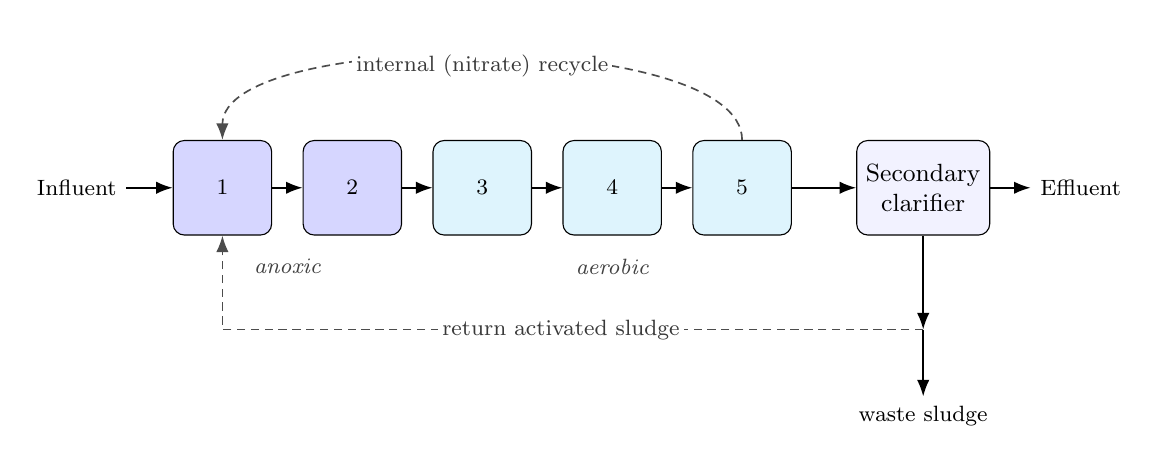
\begin{tikzpicture}[
      >={Latex[length=2.1mm]},
      unit/.style={draw, rounded corners, align=center, font=\small,
                   fill=blue!5, minimum width=16mm, minimum height=12mm},
      anoxic/.style={draw, rounded corners, align=center, font=\footnotesize,
                     fill=blue!16, minimum width=12.5mm, minimum height=12mm},
      aerobic/.style={draw, rounded corners, align=center, font=\footnotesize,
                      fill=cyan!13, minimum width=12.5mm, minimum height=12mm},
      io/.style={align=center, font=\footnotesize},
      flow/.style={->, semithick},
      recyc/.style={->, semithick, densely dashed, gray!60!black},
      rlbl/.style={font=\footnotesize, text=gray!45!black, fill=white, inner sep=1.4pt},
      zlbl/.style={font=\footnotesize\itshape, text=gray!50!black},
    ]
    \node[io]      (inf) at (-1.15,0) {Influent};
    \node[anoxic]  (r1)  at (0.7,0)   {1};
    \node[anoxic]  (r2)  at (2.35,0)  {2};
    \node[aerobic] (r3)  at (4.0,0)   {3};
    \node[aerobic] (r4)  at (5.65,0)  {4};
    \node[aerobic] (r5)  at (7.3,0)   {5};
    \node[unit]    (sc)  at (9.6,0)   {Secondary\\clarifier};
    \node[io]      (eff) at (11.6,0)  {Effluent};

    \draw[flow] (inf) -- (r1);
    \draw[flow] (r1)  -- (r2);
    \draw[flow] (r2)  -- (r3);
    \draw[flow] (r3)  -- (r4);
    \draw[flow] (r4)  -- (r5);
    \draw[flow] (r5)  -- (sc);
    \draw[flow] (sc)  -- (eff);

    \node[zlbl] at (1.525,-1.0) {anoxic};
    \node[zlbl] at (5.65,-1.0)  {aerobic};

    \draw[recyc] (r5.north) to[out=90,in=90,looseness=0.55] (r1.north);
    \node[rlbl] at (4.0,1.55) {internal (nitrate) recycle};

    \coordinate (uf) at (9.6,-1.8);
    \draw[flow]  (sc.south) -- (uf);
    \draw[recyc] (uf) -- (0.7,-1.8) -- (r1.south);
    \node[rlbl] at (5.0,-1.8) {return activated sludge};
    \draw[flow]  (uf) -- ++(0,-0.85) node[io, below] {waste sludge};
  \end{tikzpicture}
  \caption{The open-loop BSM1 plant. Five activated-sludge reactors (two anoxic,
  three aerobic) precede a ten-layer secondary clarifier, with an internal
  nitrate recycle from the last reactor to the first and the return activated
  sludge from the clarifier underflow (both resolved by
  Eq.~\eqref{eq:flow-fixedpoint}). The whole flowsheet is assembled into one
  differentiable system and integrated under a single stiff solve.}
  \label{fig:bsm1flowsheet}
\end{figure}

The verification plant (Figure~\ref{fig:bsm1flowsheet}) is the open-loop BSM1 benchmark \citep{copp2002, alex2008}, which includes five activated-sludge reactors (two anoxic and three aerated), followed by a ten-layer secondary settler, with the internal recycle and the return sludge resolved by Eq.~\eqref{eq:flow-fixedpoint}. Open-loop here means the plant runs without controllers, such that the aeration coefficients and the pumped flows are held at fixed setpoints. The activated sludge model carries the published BSM1 parameter set. The benchmark specifies those parameters at its operating temperature of fifteen degrees Celsius, as fixed values rather than as a temperature law. The engine references its rate corrections to twenty degrees, so the published fifteen-degree values are applied at that reference, where the temperature correction is unity, and the benchmark kinetics are reproduced exactly. The engine's temperature correction of parameter values, a per-parameter \(\vartheta^{T-T_{\mathrm{ref}}}\) factor, is therefore inactive in this reproduction and is not exercised by any result here; the separate \texttt{arrhenius()} rate function is not used by the ASM1 model. This is the appropriate handling for a model defined by fixed-temperature parameters, as distinct from a plant-wide model that carries an explicit temperature law and heat balance. The aeration coefficients and the oxygen saturation are the benchmark values. The ten-layer settler follows the benchmark settler model \citep{takacs1991}, which models a vertical stack of layers that exchange solids with their neighbours by bulk flow and a settling flux, so its state is the per-layer concentrations rather than a single well-mixed value. The solubles are carried through the layers, so the clarifier liquid volume holds and damps the soluble effluent signal, and the outlet particulate composition is taken from the instantaneous feed scaled by the outlet-adjacent solids concentration. Both are properties of the dynamic response only and leave the steady state unchanged.

\subsection{Anaerobic digester configuration}
\label{sec:methods-digesterconfig}

The verification reactor is an anaerobic digester. The digester model is the Anaerobic Digestion Model No.~1 \citep{batstone2002} in the form used by the plant-wide benchmark BSM2 \citep{jeppsson2007, gernaey2014}, with twenty-six soluble and particulate liquid states and three gas-phase states. Its rate laws are gated by the pH-dependent switching and inhibition functions of the expression language, evaluated at the state-derived charge-balance pH of Section~\ref{sec:methods-conditions}, so the acid--base chemistry is solved and differentiated as part of the model rather than supplied as a constant input value. The unit has a liquid volume of \(3400\)~m\(^3\) and is fed at \(178.5\)~m\(^3\)/d with the benchmark digester-feed composition, giving a nominal retention time of \SteadySRTnominal~days. This configuration is used for the steady-state solver and the washout fold of Section~\ref{sec:results-steadysolver}, where the digester steady state is also verified against the published BSM2 reference and the state-derived pH against an independent electroneutrality calculation.

\subsection{Batch and respirometric calibration studies}
\label{sec:methods-calibstudy}

The calibration and identifiability demonstrations are numerical experiments where a known parameter set is fixed, the model generates the observations from it, and the estimator is tasked with recovering the original parameter set. Because the data come from the same model, the recovery is checked against a known truth, which isolates the estimator from model structural error. The synthetic observations come from \CalNbatch\ simulated closed-batch assays of the same activated-sludge reactor that differ only in their initial state, and the design recovers \CalNfree\ heterotroph parameters of the activated-sludge model, namely the aerobic and anoxic growth rates through \(\mu_H\) and \(\eta_g\), the yield \(Y_H\), the decay rate \(b_H\), and the hydrolysis rate \(k_h\). One is an aerobic respirogram that resolves the oxygen-uptake transient. Two are anoxic denitrification assays, one substrate-limited and one nitrate-limited, that resolve the anoxic kinetics. The aerobic respirogram runs for \CalTAerH~h and the nitrate- and substrate-limited anoxic assays for \CalTNlimH\ and \CalTSlimH~h. Each assay is sampled \CalNsampAssay\ times on substrate, dissolved oxygen, and nitrate, uniformly for the anoxic assays and, for the aerobic one, with \CalAerDenseN\ samples in its first \CalAerDenseMin~min, where the oxygen falls fastest, giving \CalNobs\ observations. Each observation carries independent Gaussian noise at a realistic sensor resolution, with standard deviations of \CalSigSS~mg~COD/L on substrate, \CalSigSO~mg~O\(_2\)/L on dissolved oxygen, and \CalSigSNO~mg~N/L on nitrate. The half-saturation constants are held at their literature values, the standard practice for batch identification. Estimation uses the library's calibration routine of Section~\ref{sec:methods-ad}, whose gradient is the discrete adjoint of the stiff batch solve. Every fit is a maximum-likelihood fit with the priors switched off, since the priors shipped with the model file are centred on the true values and would pull the estimate toward them. The Monte Carlo recoveries (Figures~\ref{fig:calibration}d and \ref{fig:identifiability}c) start each fit from a random point, with every free parameter set to its true value multiplied by \(\exp(\CalStartSpread\,z)\), \(z\sim\mathcal{N}(0,1)\), roughly \(\pm40\%\), and the two fractions \(\eta_g\) and \(Y_H\) clipped to \((0.05,0.95)\); the optimizer (L-BFGS-B) runs from that single start. Two quantities characterize the design rather than the estimator and are computed from the true values: the Fisher information of Figure~\ref{fig:identifiability}a--b and of the experiment design of Figure~\ref{fig:design} is evaluated at the true values, and at each point of the profile likelihood (Figure~\ref{fig:identifiability}d) the parameters other than \(\mu_H\) start from their true values.

A companion configuration applies the same estimator to real measurements, where model structural error also enters. The data are \RespNww\ aerobic respirograms of filtered municipal wastewater, one each of raw wastewater, primary-clarifier effluent, and rotating-belt-filter effluent. Each dataset is an oxygen-uptake-rate transient digitized from an independent respirometric study: all three are the Run~1 respirograms of Figure~4-1 of \citet{gupta2018thesis}, whose Table~4-2 also gives the biomass, COD fractionation and growth rates reported for them. The raw-wastewater and rotating-belt-filter respirograms were also published in \citet{gupta2018}. Two heterotroph structures are calibrated to them and swapped by editing the model YAML file alone. The first is a reduced ASM1 aerobic core with death regeneration, in which aerobic growth on readily biodegradable substrate is the only oxygen-consuming process. The other is a modified ASM3 structure with simultaneous storage and growth \citep{karahangul2003}, in which substrate is both grown on directly and stored as an internal polymer that is respired later. Both fix the yield \(Y_H=\RespYH\) and the decay rate \(b_H=\RespBH\)~d\(^{-1}\), and each fixes the half-saturation \(K_S\) at the standard value for its own structure: \(\RespKSdr\)~mg\,COD\,L\(^{-1}\) for the reduced (ASM1) model and \(\RespKSst\)~mg\,COD\,L\(^{-1}\) for the storage (ASM3) model \citep{henze2000}. The active biomass \(X_H\) is fixed at the value reported by the source study for each wastewater, since \(\mu_H\) is identifiable from a single respirogram only when \(X_H\) is fixed. The reduced model then frees \(\mu_H\), a hydrolysis rate, and the initial readily and slowly biodegradable COD, \(S_{S,0}\) and \(S_{H,0}\), as two independent initial pools. Their total is not tied to the source study's COD fractionation, which is itself a model-derived estimate. The storage model frees \(\mu_H\), the storage and stored-growth rates, and the initial readily biodegradable COD. Every fit uses the library's calibration routine of Section~\ref{sec:methods-ad}, with the oxygen uptake rate written as an observation function of the state and the priors off. Each fit is located by a multistart over a fixed grid of starting values, run as a least-squares fit, and the best start is refined as a maximum-likelihood fit with the noise level fixed at that fit's residual root-mean-square, which gives the Laplace uncertainty and the likelihood scale of the profile. This configuration is used for the model-structure comparison of Section~\ref{sec:results-diff}.

\subsection{Reproducibility}
\label{sec:methods-repro}

Every analysis in this paper can be reproduced from the provided code and data. The computations are deterministic, with every noise realization and random start drawn from a fixed seed, except the wall-clock timings, which vary from run to run and are reported as medians with their spread. All computations in this paper, and so all timings reported, were run on a single MacBook Pro with an Apple M3 Pro processor (11 CPU cores, 5 performance and 6 efficiency) and 18~GB of unified memory, under macOS~26.3, on the JAX CPU backend in double precision (JAX~0.10.2, Python~3.13). Each analysis runs its computation once, against the pinned \texttt{aquakin} release of the code metadata below, and caches the result. The scripts refuse to compute against any other commit or a locally modified checkout, and every cached result records the commit it was computed with. The cached results feed all of the generated tables and figures, and macros supply every computed number in the text, so no reported result is entered by hand and none can go stale. Inputs that the analyses take as given, such as tolerances, volumes and flows, are written in the text directly. The parameter set and the published reference values are shipped with the paper as data, so the benchmark distribution itself is not needed to reproduce the validation.

% =========================================================================
\section{Results}
\label{sec:results}

The code and its implementation are evaluated in the subsections that follow. Section~\ref{sec:results-verification} verifies that the implementation is correct, against a closed-form solution, against a stoichiometric conservation audit, and against finite-difference gradients. Sections~\ref{sec:results-steady} and \ref{sec:results-dynamic} validate the assembled BSM1 plant against the published benchmark at steady state and across the dry-weather dynamic. Section~\ref{sec:results-steadysolver} demonstrates the differentiable steady-state solver and the digester washout fold. Section~\ref{sec:results-diff} demonstrates the calibration and sensitivity features which become direct gradient computations because of the differentiability of the code. Section~\ref{sec:results-performance} reports the cost of compilation, of a solve, and of a gradient.

\subsection{Verification}
\label{sec:results-verification}

Verification proceeds in two stages: against closed-form analytical references on small test problems, then against finite differences and an independent forward-mode gradient on the assembled BSM1 plant.

\subsubsection{Analytical verification}
\label{sec:results-verification-analytic}

The code is first verified using a single-reaction model with a closed-form solution. First-order decay \(A\rightarrow B\) with rate \(k[A]\) is a two-species system whose stoichiometry conserves the total \([A]+[B]=[A]_0\) exactly; its closed-form solution is \([A](t)=[A]_0 e^{-kt}\), \([B](t)=[A]_0-[A](t)\). Integrating this model with the stiff solver, at a solver tolerance of \(\mathrm{rtol}=\VerifRtol\) and \(\mathrm{atol}=\VerifAtol\), matches the analytical solution to a maximum relative error of \VerifDecayMaxRelErr\ over the trajectory (Figure~\ref{fig:verification}a). The derivative of the same solution with respect to the rate constant is taken by the discrete adjoint and, at the same tolerance, matches the analytical derivative \(-t[A]_0 e^{-kt}\) to a relative error of \VerifDecayGradRelErr. That residual belongs to the solver, not the gradient calculation. Because the reverse-mode gradient is the exact gradient of the discrete solve, tightening the solver tolerance drives its disagreement with the analytical derivative down alongside the solver tolerance. This error falls with the solution error, by about a factor of ten per decade of tolerance, down to the tightest tolerance tried, \(10^{-15}\), where the gradient error is \VerifGradTolFloor\ (Figure~\ref{fig:verification}b); neither curve has reached the float64 floor. The gradient error therefore stays proportional to the solver tolerance, within a small factor of it, and the gradient adds no error of its own. The looser default tolerance used in the rest of the paper trades this precision for speed.

\begin{figure}[htbp]
  \centering
  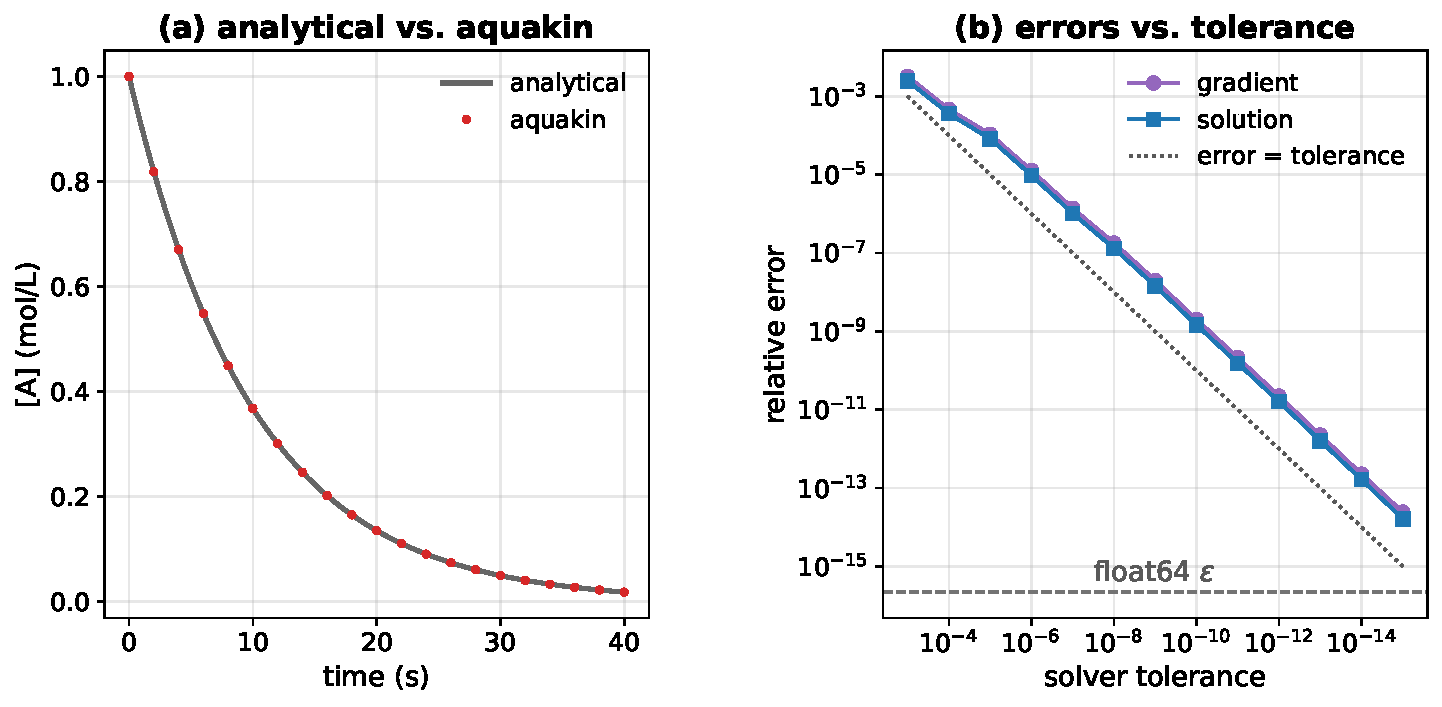
\includegraphics[width=\linewidth]{fig_verification}
  \caption{Verification of the code. (a) The integrated first-order decay matches
  the closed-form solution. (b) Relative errors of the solution and the reverse-mode
  derivative with respect to the rate constant at \(t=25\), as the solver tolerance is tightened, with \(\mathrm{rtol}=\mathrm{atol}\) set to the value on the axis.
  Both fall in proportion to the tolerance down to the tightest tolerance tried
  (the gradient error reaches \VerifGradTolFloor\ at \(10^{-15}\)).}
  \label{fig:verification}
\end{figure}

Mass is confirmed to be conserved to round-off error by observing the integrated total \([A]+[B]\), which drifts by at most \VerifConsTotalMax\ from \([A]_0\) over the trajectory. This is the stoichiometric conservation established above holding to floating-point precision.

A stiff linear chain \(A\rightarrow B\rightarrow C\) with a rate ratio of \VerifStiffRatio\ gives a second stiff closed-form reference and therefore a closed-form parameter sensitivity. The discrete adjoint is taken on its stiff solve in the large-step regime it is built for, where the adaptive solver takes a median implicit step \VerifStiffStepRatio\ times the fastest reaction timescale (measured on a separate forward Kvaerno5 solve at the same tolerances), with no step-size limitation. It matches that analytic sensitivity to \VerifStiffGradRel  with tolerances of \(\mathrm{rtol}=\VerifRtol\) and \(\mathrm{atol}=\VerifAtol\). The gradient calculation is therefore verified against an analytic reference on a stiff problem, as well as the non-stiff problem considered above.

\subsubsection{Finite-difference verification}
\label{sec:results-verification-fd}

Verification now moves to the assembled BSM1 plant, where no closed-form reference exists. The plant is described in Section~\ref{sec:methods-bsm1config} and contains five activated-sludge reactors and a ten-layer settler. The influent is the official BSM1 open-loop steady-state constant influent specification and all parameters are matched with those in the BSM1 published parameters. When the plant is integrated to \VerifADFDHorizon\ days the scaled residual (Eq.~\eqref{eq:scaled-residual}) is \VerifADFDHorizonResid\ and the plant-wide mass balance at that steady state closes to a relative residual of \VerifMassBalCOD\ in COD and \VerifMassBalN\ in nitrogen. Two processes cross the liquid/gas boundary rather than transforming dissolved mass: aeration supplies the oxygen that the COD balance consumes, and denitrification releases nitrogen as dinitrogen gas, which the model does not carry as a species. The conservation audit of Section~\ref{sec:methods-safety} accounts for both. Of the \ConsNreactions\ ASM1 reactions it flags only anoxic heterotroph growth, with residuals of \ConsResidN\ in nitrogen and \ConsResidCOD\ in COD per unit of biomass COD formed. Both are the dinitrogen released, \((1-Y_H)/(2.86\,Y_H)\) of nitrogen carrying \ConsNtwoCODperN~g COD per g N relative to the ammonia reference of the composition table. Aerobic growth, whose electron acceptor is the dissolved oxygen that aeration supplies, balances to round-off, as do the decay, hydrolysis and ammonification reactions. Autotrophic growth leaves a COD residual of \ConsAutoResidCOD, below the reporting tolerance, from the rounding of the nitrification oxygen demand to 4.57 in the ASM1 stoichiometry. Together, the plant-wide mass balance and the audit confirm that the stoichiometry carries no error and that the solver has converged to a steady state.

The end-to-end gradient is then verified against finite differences at this same operating point. The test quantity is a scalar loss, a sum of squared effluent concentrations, computed as a function of \VerifADFDNParams\ activated-sludge kinetic parameters: the heterotroph and autotroph growth rates \(\mu_H\) and \(\mu_A\), the heterotroph decay rate \(b_H\), the heterotroph yield \(Y_H\), and the anoxic growth correction factor \(\eta_g\). The loss represents the effluent at the steady state above, at a tightened solver tolerance of \(\mathrm{rtol}=\mathrm{atol}=10^{-10}\) so it is accurate enough for the finite-difference comparison; both are pinned explicitly, since leaving \(\mathrm{atol}\) at its auto-scaled default becomes the binding constraint once \(\mathrm{rtol}\) is tightened. The loss is differentiated by the discrete adjoint, which gives its exact reverse-mode gradient. It is also differentiated by a central finite difference, which perturbs each parameter up and down in turn, re-solves the plant, and estimates the slope from the resulting change in loss. A step-size sweep for each parameter (Figure~\ref{fig:plantfd}) traces the classic truncation-versus-noise trade-off. First, the disagreement falls as the step shrinks from a large value, reaches a minimum, then rises again once the step is small enough that floating-point cancellation dominates. At the step \VerifADFDHDefault\ near that minimum, the two gradients agree to \VerifADFDMaxRelErr\ in the relative Euclidean norm across the five parameters. The largest per-parameter disagreement at that point is \VerifADFDWorstRel, for \VerifADFDWorstName. This residual is set by the finite-difference step, not by the automatic differentiation. Figure~\ref{fig:plantfd} shows that the chosen step sits at the minimum of the error curve only for \(\eta_g\). For the other four parameters it is still on the truncation-limited slope, and a smaller step would lower their finite-difference error further, so the agreement reported here is conservative. The agreement confirms that the gradient propagated through the assembled plant, across the recycle loops and the settler, is the gradient of the same function the solver integrates.

\begin{figure}[htbp]
  \centering
  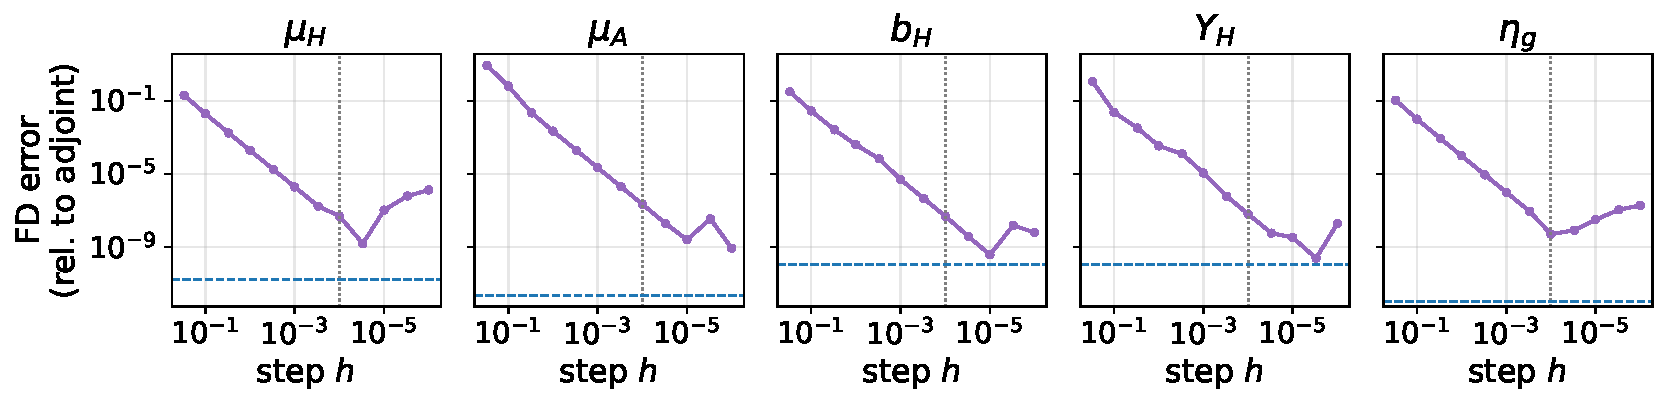
\includegraphics[width=\linewidth]{fig_plant_fd}
  \caption{Plant gradient verified against finite differences: step-size sweep,
  per parameter. For each of the \VerifADFDNParams\ activated-sludge parameters
  of the test loss, the relative difference between the reverse-mode
  (discrete-adjoint) gradient and a central finite difference, as the
  finite-difference step \(h\) is swept, a perturbation of \(h\max(\lvert\theta_j\rvert,1)\) to parameter \(\theta_j\) (dotted vertical line: the step
  \VerifADFDHDefault\ used for the residual reported in
  Section~\ref{sec:results-verification-fd}). Each curve falls as \(h\)
  shrinks from a large value (truncation-limited), reaches a minimum, then
  rises again as floating-point cancellation dominates at very small \(h\). The dashed horizontal line is the no-finite-difference
  reference for that parameter, the forward-mode-versus-adjoint agreement of
  Section~\ref{sec:results-verification-fd}: it sits below every curve's own
  floor, confirming that finite differencing, not the gradient, sets the
  floor.}
  \label{fig:plantfd}
\end{figure}

Finite differencing cannot eliminate its error, it can only bound it, so a further check verifies the plant gradient without any finite-difference reference at all. The same effluent loss, at the same operating point and with respect to the same five parameters, is differentiated a third way: by forward-mode automatic differentiation. Forward mode and the discrete adjoint are two independent algorithms for the same derivative, and they agree to \VerifPlantFwdRevRel, about \VerifFwdRevRatio$\times$ tighter than the finite-difference comparison above. The looser finite-difference agreement is therefore a property of finite differencing and not of the gradient.

\subsection{Steady-state numerical equivalence with BSM1}
\label{sec:results-steady}

The assembled open-loop BSM1 plant (Section~\ref{sec:methods-bsm1config}) reproduces the published benchmark steady state closely in every reactor and in the settler (Table~\ref{tab:steady}). The plant is the five activated-sludge reactors and the ten-layer settler, driven to steady state by forward integration under the constant influent, with the activated sludge model carrying the published BSM1 parameter values applied at the engine reference temperature. Across the \SteadyNquant\ resolvable reactor quantities of the five reactors, the worst relative difference from the published reference is \SteadyReactorWorstPct\,\%. These are the reactor states compared on a relative basis, excluding those whose reference value is below \(10^{-2}\) (the dissolved oxygen in the two anoxic reactors), which a relative difference cannot resolve, and the suspended solids, a derived sum of the particulate states that is compared in the settler instead. The settler effluent agrees to within \SteadyEffWorstPct\,\% and the ten-layer settler solids profile to within \SteadyTSSWorstPct\,\%, and the plant-wide mass balance closes to a relative residual of \VerifMassBalCOD\ in COD. Figure~\ref{fig:steady} shows the reactor composition and the settler profile against the reference. Because the plant is run with the benchmark's own parameters against the benchmark's own reference solution, this is a numerical-equivalence check rather than an independent validation of model fidelity. Agreement at this level establishes that the ASM1 stoichiometry and kinetics, the recycle resolution of Eq.~\eqref{eq:flow-fixedpoint}, and the non-reacting settler are implemented correctly against a reference implementation. The physical standing of the model is the benchmark's own and is not re-established here. What is shown is that the engine reproduces the benchmark's results.

\begin{figure}[htbp]
  \centering
  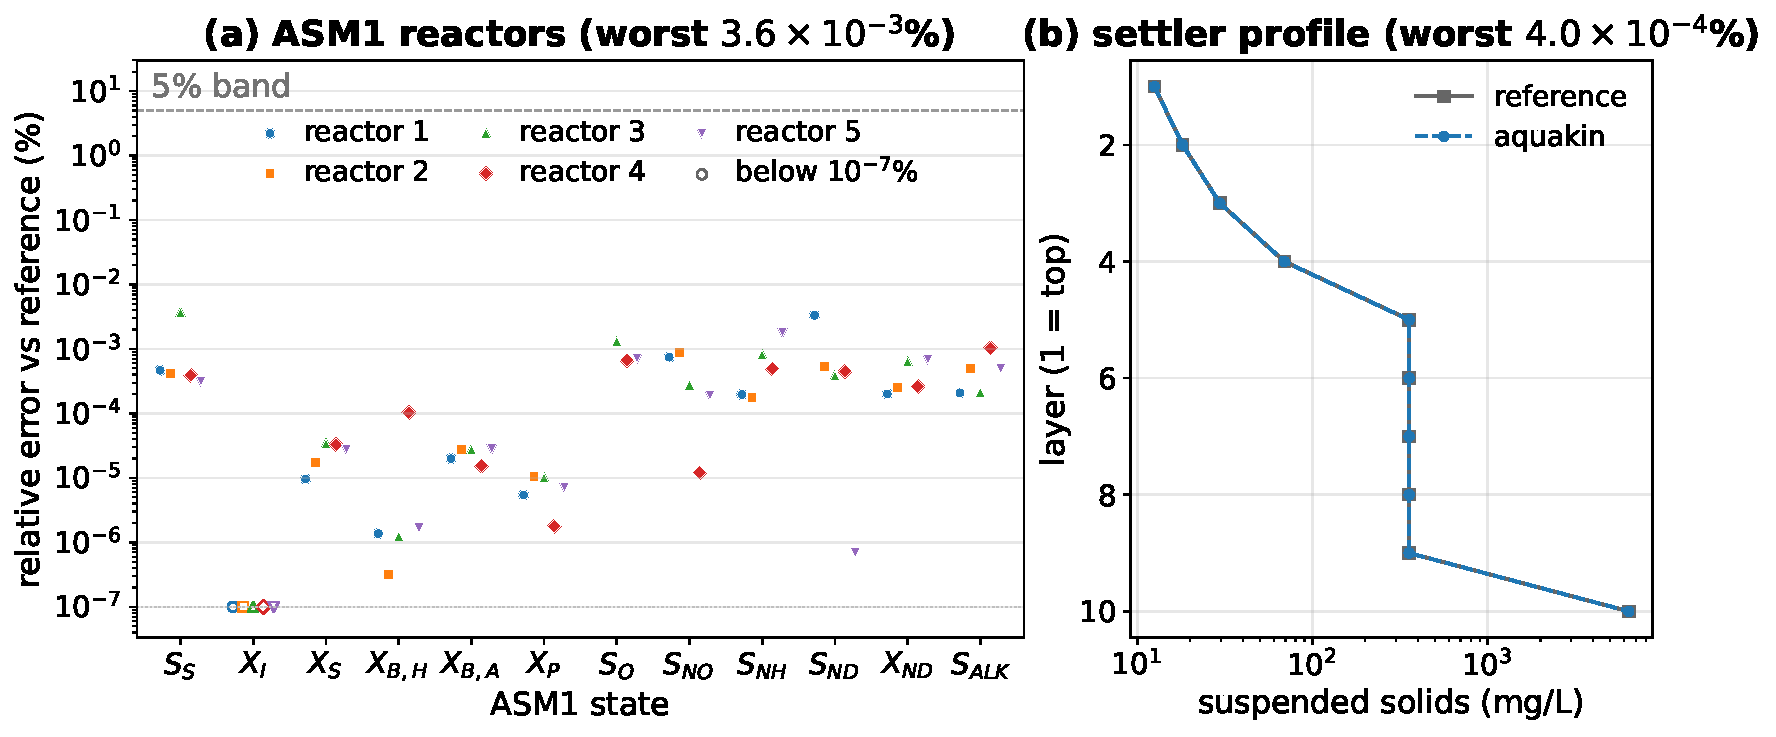
\includegraphics[width=\linewidth]{fig_bsm1_steady}
  \caption{Open-loop BSM1 steady-state numerical equivalence. (a) The relative error
  of each of the \SteadyNquant\ resolvable activated-sludge reactor quantities against
  the published benchmark steady state, on a logarithmic axis; every quantity agrees
  far inside the \(5\%\) engineering band, at the precision the benchmark
  reference values are reported to. Quantities that agree to better than \(10^{-7}\,\%\) are drawn
  hollow on the dotted floor line. (b) The ten-layer settler suspended-solids profile
  from top to bottom, model and reference. The reference is the open-loop steady state
  of the benchmark Matlab/Simulink implementation.}
  \label{fig:steady}
\end{figure}

\subsection{Dynamic numerical equivalence with BSM1}
\label{sec:results-dynamic}

The same plant reproduces the dry-weather dynamic benchmark to a fraction of a percent. Following the benchmark protocol, the plant is brought to steady state on the constant influent, warmed for a further fourteen days on the dry-weather influent, and then scored over days seven to fourteen of a second fourteen-day dry run, with the effluent averaged on a flow-weighted load basis. The averaged effluent ammonia is \DynEffSNH~mg~N/L against the reference \DynEffSNHRef, the total nitrogen is \DynEffTN\ against \DynEffTNRef, the total COD is \DynEffCOD\ against \DynEffCODRef, and the suspended solids are \DynEffTSS\ against \DynEffTSSRef. The largest difference among these averaged effluent quantities is \DynEffWorstPct\,\%. The effluent quality index is \DynEQI\ against the reference \DynEQIRef, a difference of \DynEQIPct\,\%, and the operational cost index is \DynOCI\ against \DynOCIRef, a difference of \DynOCIPct\,\%. Both are scored on the \emph{updated} benchmark index convention, the revision of the original BSM1 indices \citep{copp2002} that adjusts the aeration and pumping energy factors and the effluent- and influent-quality weightings \citep{gernaey2014}. This is the convention the engine's benchmark evaluation implements, and the model is compared against the reference values for the same convention, which the tables label accordingly (the averaged effluent concentrations above are convention-independent). The benchmark reports these flow-weighted day-seven-to-fourteen averages rather than a reference effluent time series, so the comparison is on the averaged loads. The model effluent trajectory the averages are taken over is shown in Figure~\ref{fig:dynamic}. Reproducing the dynamic effluent ammonia at this level requires the secondary settler to follow the benchmark ten-layer settler model \citep{takacs1991} in two respects that leave the steady state unchanged and matter only dynamically. The soluble species are carried through the settler layers, so the clarifier liquid volume damps the dynamic soluble effluent signal (the soluble holdup of the BSM1 reference settler, \texttt{settler1dv4}), and the outlet particulate composition is set from the instantaneous feed scaled by the boundary-layer solids rather than from a per-layer composition memory. The effect is not cosmetic: with the common pass-through settler that carries no soluble holdup, the averaged effluent ammonia rises to \DynSnhNoHoldup~mg~N/L, about \DynHoldupReldiff\,\% above the benchmark. Two effects combine, and comparing time averages with flow-weighted ones separates them. About a third of the rise (\DynHoldupMeanSharePct\,\%) is a higher time-averaged effluent ammonia. Without the holdup, the last reactor itself runs at a higher average ammonia (\DynTankFiveNoHoldup\ rather than \DynTankFiveHoldup~mg~N/L), while with the holdup the clarifier raises its effluent's time average above that of its feed, offsetting part of the reactor difference. The other two-thirds (\DynHoldupFlowSharePct\,\%) comes from the flow weighting the benchmark scores. Without the holdup, the effluent ammonia peaks coincide with the flow peaks and carry more weight, whereas the clarifier delays the damped signal slightly out of phase with the flow (Figure~\ref{fig:dynamic}c), so that its flow-weighted average falls below its time average. Carrying the solubles through the clarifier volume, as the benchmark settler does, recovers the reference average. Figure~\ref{fig:dynamic}b plots the effluent-ammonia series with and without the holdup against the reference average, and Figure~\ref{fig:dynamic}c shows the clarifier damping directly. The plant reproduces the benchmark dynamics to within a fraction of a percent in every reported average.

\begin{figure}[htbp]
  \centering
  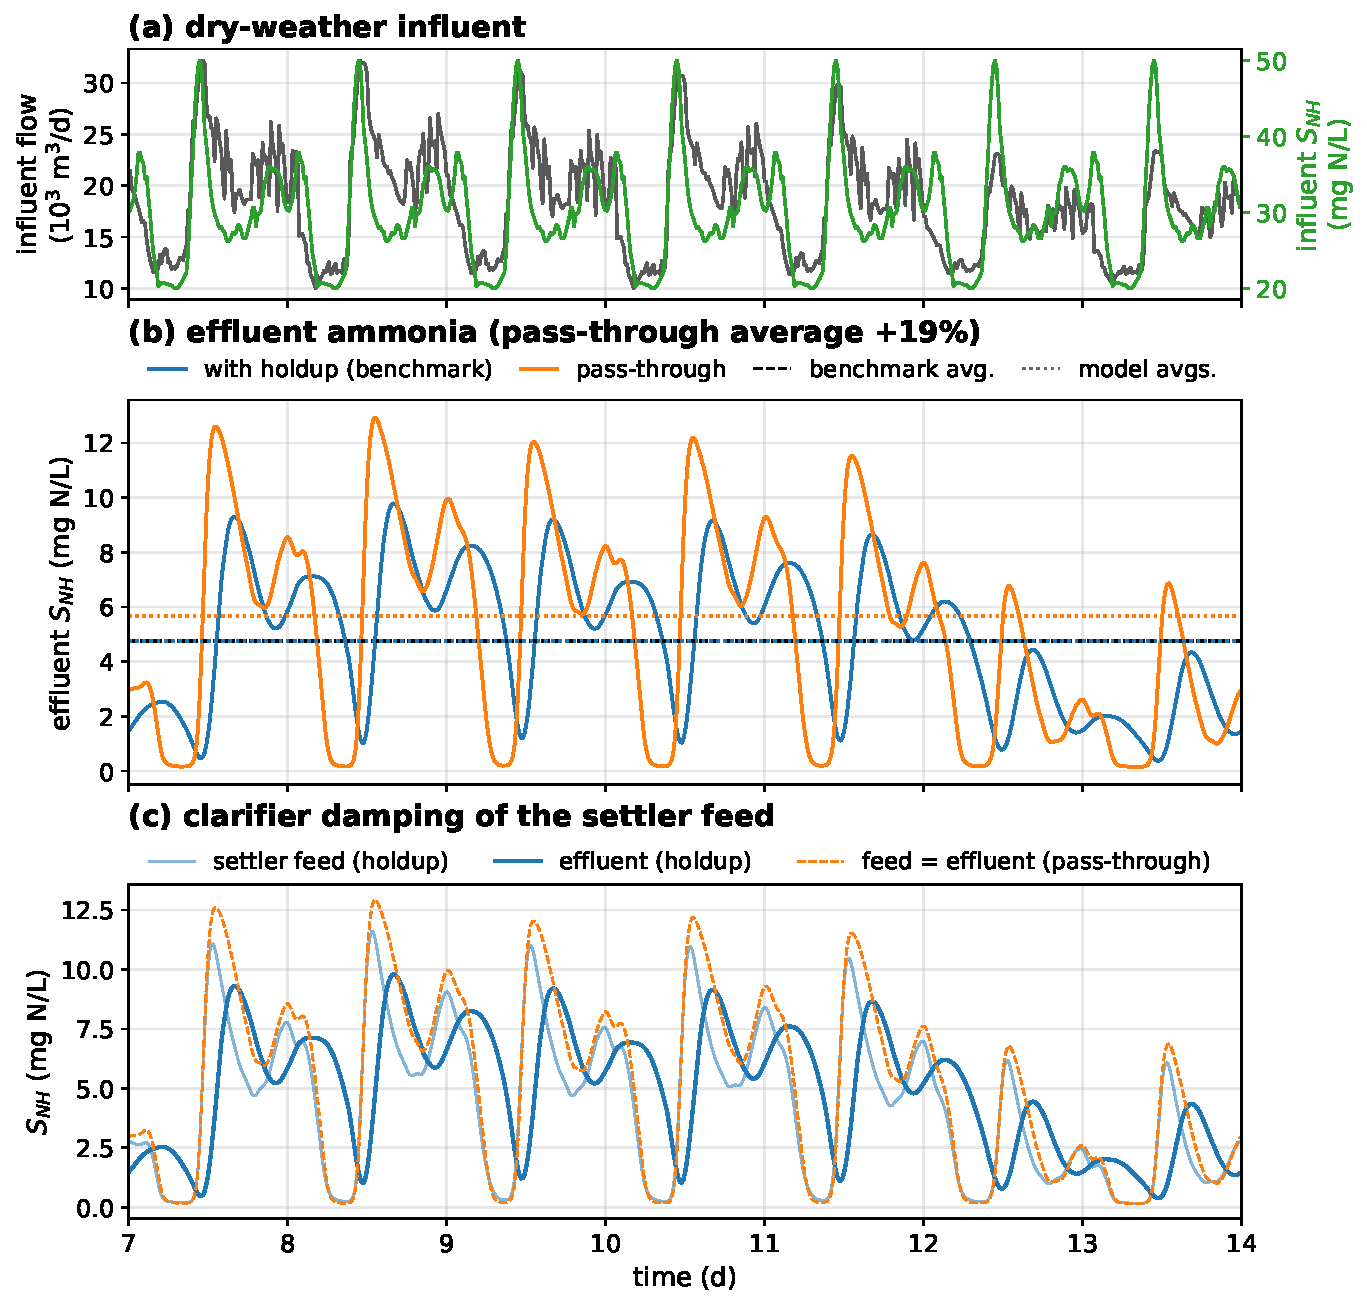
\includegraphics[width=\linewidth]{fig_bsm1_dynamic}
  \caption{Open-loop BSM1 dynamic reproduction under the dry-weather influent, days
  seven to fourteen, and the role of the settler soluble holdup. (a) The dry-weather
  influent flow and ammonia that drive the diurnal cycle. (b) Effluent ammonia computed
  with the benchmark's soluble-carrying settler and with a common pass-through settler.
  The dashed line is the benchmark's flow-weighted average and the dotted lines are the
  two model averages; the benchmark-settler average coincides with the reference, while
  the pass-through average is \DynHoldupReldiff\,\% higher. The benchmark reports only
  this average, not a time series, so the agreement is on the averaged quantities
  (Table~\ref{tab:dynamic}). (c) What the clarifier volume does to the signal: with the
  holdup the effluent is a damped, delayed copy of the settler feed, while the
  pass-through settler passes its feed straight to the effluent.}
  \label{fig:dynamic}
\end{figure}

\subsection{The steady-state solver}
\label{sec:results-steadysolver}

Before demonstrating the solver on the anaerobic digester, we establish that the digester model and the pH it depends on are themselves correct. Run as a standalone unit on the published BSM2 digester feed (Section~\ref{sec:methods-digesterconfig}), the ADM1 steady state, found as the algebraic root by the solver below and cross-checked against \SteadyFwdHorizon~days of forward integration to the same attractor (both converged below the PTC tolerance on the scaled residual of Eq.~\eqref{eq:scaled-residual}, and agreeing to a largest relative difference of \DigPtcVsFwd\ over the states above \(10^{-3}\)), reproduces the published BSM2 open-loop digester composition to a worst relative difference of \DigWorstPct\,\% across the \DigNresolvable\ resolvable states, the largest on the \DigWorstName, the most pH-sensitive state, and the methane within \DigMethanePct\,\% (per state in Section~\ref{si:validation}, Table~\ref{tab:si-digester}). The state-derived charge-balance pH is verified on the same footing: at the converged composition the engine solves pH~\DigPH, matching an independent electroneutrality calculation with the published ADM1 acid--base constants (carbonate, ammonia, the four volatile-fatty-acid systems, and the strong ions) to \(\lvert\Delta\text{pH}\rvert=\DigPHAbsErr\). This is a numerical-equivalence check of the standalone digester against the benchmark reference, on the same footing as the BSM1 reproduction; the full coupled BSM2 plant-wide validation is out of scope here. The demonstrations that follow therefore run on a verified digester and a verified pH.

The steady states solved thus far have been reached by forward integration, but the engine can also find them directly using its steady-state solver. We demonstrate this on the anaerobic digester (Section~\ref{sec:methods-digesterconfig}), whose long retention time makes forward integration slow. Pseudo-transient continuation (Eq.~\eqref{eq:ptc}) reaches the digester steady state in \SteadyPtcIters\ iterations to a scaled residual (Eq.~\eqref{eq:scaled-residual}) of \SteadyPtcResidual, the same root as the forward-integrated steady state of the validation above. Once compiled, each root find is about an order of magnitude faster per solve than forward integration. The forward solve is stable at about \SteadyFwdSolveMs~ms, whether run to a fixed \(\SteadyFwdHorizon\)-day horizon or stopped once its scaled residual reaches the PTC convergence tolerance of \(\PtcTol\) (at about \SteadyFwdMatchDays\ simulated days), while the sub-millisecond root find is \SteadyPtcSpeedupLo--\SteadyPtcSpeedupHi$\times$ faster per solve: the forward median divided by the 90th and the 10th percentile of the root find's \SteadyNruns\ timed solves (Figure~\ref{fig:steadysolver}a). The one-time compilation is a separate cost, paid once and amortized over the many solves a continuation or a calibration performs. Beyond its per-solve speed, the root find returns the steady state as a differentiable algebraic object, whose sensitivities follow from the implicit function theorem (Eq.~\eqref{eq:ift}) at the root. The sensitivity of the steady acetate concentration to the acetate-uptake rate obtained this way matches a central finite difference to \SteadySensRel. Forward- and reverse-mode differentiation return the same implicit-function tangent by construction, so their agreement to machine precision is not an independent check.

These sensitivities matter most near the limits of a process, where the operating point is about to be lost. For an anaerobic digester the classic such limit is washout under overloading. As the feed flow rises the retention time falls, and the slowest-growing populations, the acetoclastic methanogens and the long-chain-fatty-acid degraders, have less time to reproduce. Past a critical loading they are flushed out faster than they grow, acetate accumulates, and methanogenesis collapses. Traced as a function of the loading, the steady state forms a branch that bends back on itself at this critical loading, a fold in the language of bifurcation theory (formally a saddle-node bifurcation) \citep{seydel2010}. Below the fold two steady states coexist at each loading: the stable methanogenic operating state, and an unstable intermediate state from which any small disturbance moves the digester away. The two merge at the fold, and beyond it no methanogenic steady state exists, so the digester drifts toward washout. The fold therefore marks the largest loading, or equivalently the shortest retention time, at which the digester can be operated, and locating it is the task of the pseudo-arclength continuation below.

Raising the feed flow from the design point, the operating branch reaches the fold at a retention time of \SteadyFoldSRT~days, down from the nominal \SteadySRTnominal~days, with the effluent acetate rising steeply as the fold is approached (Figure~\ref{fig:steadysolver}b). A direct root find, warm-started at each loading from the previous solution, follows the stable branch only while it exists. It fails just past the fold, at \SteadyFoldFailDil\ times the design loading: the methanogenic branch it was following ends at the fold, and from the last methanogenic solution the root find does not converge to the washed-out steady state that remains. The pseudo-arclength continuation of Section~\ref{sec:methods-steady} instead follows the branch by its arclength rather than by the loading. Its augmented Jacobian (Eq.~\eqref{eq:bordered}) stays non-singular at the fold, so it rounds the fold and continues back along the unstable branch (dashed in Figure~\ref{fig:steadysolver}b). Neither forward integration nor a direct root find can reach that branch.

A point on the unstable branch is a steady state in the mathematical sense, with every production and removal rate in balance, but not one at which the digester can be operated. Each is a saddle: its Jacobian has exactly one eigenvalue with positive real part, while those of the stable branch all have negative real parts. Physically, the unstable state carries a smaller acetoclastic population than the stable state at the same loading. At a feed-flow multiplier of \SteadyUnsLam\ it holds \SteadyUnsXacUns\ against \SteadyUnsXacSt~kg~COD~m\(^{-3}\) of acetoclastic methanogens, just enough that their growth on the much higher acetate, \SteadyUnsSacUns\ against \SteadyUnsSacSt~kg~COD~m\(^{-3}\), balances their washout. Its inorganic carbon is depleted to \SteadyUnsSicUns\ against \SteadyUnsSicSt~kmol~C~m\(^{-3}\) as the accumulated acid consumes the alkalinity. The higher effluent acetate of the dashed branch is therefore not a second operating point but a threshold. Started from the unstable state and moved \SteadyUnsNudgePct\,\% of the way toward the stable one, the digester returns to the stable state; moved \SteadyUnsNudgePct\,\% the other way, it loses its acetoclastic methanogens entirely and the acetate rises to \SteadyUnsSacWash~kg~COD~m\(^{-3}\), identifying a third, washed-out steady state that coexists at the same loading. The unstable state thus lies on the boundary between the region of states that recover to stable operation and the region that fails to washout, and its distance from the stable state indicates how large a disturbance, such as a shock load or an inhibition that depletes the methanogens, the digester can absorb. At the design loading that margin is wide, with the unstable acetate at \SteadyUnsSacDesUns\ against \SteadyUnsSacDesSt~kg~COD~m\(^{-3}\) in operation. At a multiplier of \SteadyUnsLamNear\ it has narrowed to \SteadyUnsSacNearUns\ against \SteadyUnsSacNearSt, and it closes at the fold, where the two states merge and an arbitrarily small upset is enough to tip the digester into washout.

The steady-state sensitivity of the acetate to the loading, the loading column of Eq.~\eqref{eq:ift}, is the slope of the branch in Figure~\ref{fig:steadysolver}b, and the engine evaluates it exactly at every point of the traced branch (Figure~\ref{fig:steadysolver}c). At the design loading it is \SteadySensDesign~kg~COD~m\(^{-3}\) per unit of the feed-flow multiplier. At the stable point nearest the fold, \SteadySensNearDist\ below it in loading (\SteadySensNearPct\,\% of the fold loading), it is \SteadySensNearFold, about \SteadySensGain\ times larger, so close to the fold a small change in loading moves the steady state a long way. On both arms it grows without bound as the fold is approached, because the Jacobian \(\mathbf{F}_{\mathbf{x}}\) becomes singular there. Near a saddle-node the branch is locally a parabola, \(\alpha\approx\alpha_f-a\,(S_{ac}-S_{ac,f})^2\), where \(\alpha_f\) is the loading at the fold (here \SteadyFoldDil) and \(S_{ac,f}\) the acetate there. The two arms are then \(S_{ac}-S_{ac,f}\approx\pm\sqrt{(\alpha_f-\alpha)/a}\), and the sensitivity grows as \((\alpha_f-\alpha)^{-1/2}\), a straight line of slope \(-1/2\) on the logarithmic axes of Figure~\ref{fig:steadysolver}c. The computed arms run parallel to that line, with local exponents of \SteadySensExpStable\ on the stable arm and \SteadySensExpUnstable\ on the unstable arm. They bracket \(-1/2\) because the next-order term in the shape of the branch flattens one arm and steepens the other. Three conclusions follow from this result. First, the exact gradient through the root find stays finite and usable right up to the fold, so the solver does not lose differentiability before the physics does. Second, the gradient diverges at the rate theory prescribes for a saddle-node, which checks the computed derivatives against a known result rather than only against a finite difference. Third, the size of the gradient is itself an early warning of washout. It can be read at the current operating point without tracing the branch, and for this digester a value of order \SteadySensNearFold\ places the loading within a fraction of a percent of the fold.

\begin{figure}[htbp]
  \centering
  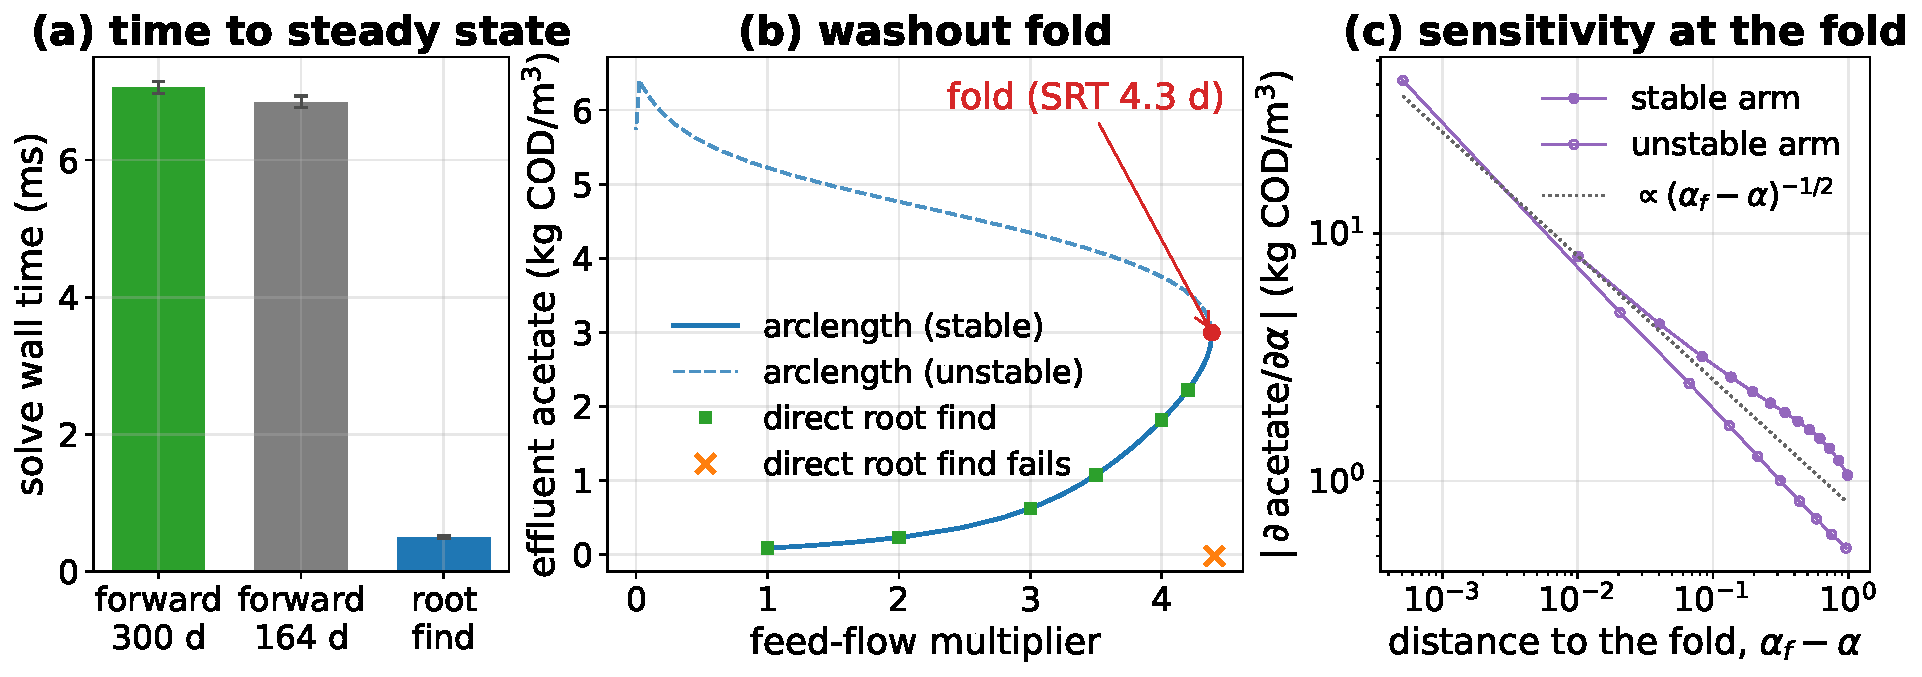
\includegraphics[width=\linewidth]{fig_steady_solver}
  \caption{The differentiable steady-state solver on the anaerobic digester. (a)
  Solve time to the steady state, the one-time JIT compilation excluded: forward
  integration to a fixed \(\SteadyFwdHorizon\)-day horizon, forward integration only to the horizon
  where it reaches the pseudo-transient continuation (PTC) convergence tolerance, and the PTC root
  find; bars are the median over \SteadyNruns\ timed runs and error bars span the 10th--90th
  percentile. Per solve the root find is about an order of magnitude faster than forward
  integration; its further value is the differentiable algebraic root and the fold
  traversal below. (b) The
  methanogenesis washout fold: effluent acetate against the feed-flow multiplier. The
  stable operating branch (solid) turns back at the fold, at a retention time of
  \SteadyFoldSRT~days, into the unstable branch (dashed). A direct root find reaches
  only the stable branch and fails past the fold, while pseudo-arclength continuation
  rounds the fold and traces the unstable branch. (c) The steady-state sensitivity of
  the acetate to the loading, evaluated exactly from the implicit function theorem
  (Eq.~\eqref{eq:ift}) at each traced branch point, against the distance to the fold
  \(\alpha_f-\alpha\): on both arms it diverges at close to the inverse-square-root rate
  of a saddle-node (dotted reference line).}
  \label{fig:steadysolver}
\end{figure}

\subsection{Calibration and identifiability with exact gradients}
\label{sec:results-diff}

The verified gradients turn calibration from a derivative-free search into a direct computation, and the same reverse-mode gradient that drives the fit also makes it cheap. We show this on a set of activated-sludge batch assays, kept apart from the full plant so the demonstration is self-contained. The first set of results in this section are a twin experiment where the observations are generated by the model itself and a known parameter set is recovered from them. Such a design establishes the correctness, the cost, and the identifiability structure of the gradient-based estimator in isolation from model structural error. We then apply the same estimator to real respirometric measurements, where structural error also enters, at the end of the section.

The \CalNfree\ heterotroph parameters ($\mu_H$, $\eta_g$, $Y_H$, $b_H$, $k_h$) are recovered jointly from the \CalNbatch\ closed-batch assays of the twin-experiment design of Section~\ref{sec:methods-calibstudy}, whose \CalNobs\ noisy observations the model itself generates from a known parameter set (Figure~\ref{fig:calibration}a--c). Across \CalNmc\ independent noise realizations, each fitted from its own random start, the recovery is unbiased to within sampling error: the largest bias, \CalWorstBias\,\% in \CalWorstBiasName, is \CalWorstBiasSE\ Monte Carlo standard errors, and every other parameter's bias is smaller relative to its spread (Figure~\ref{fig:calibration}d). A single noise-free recovery shows only that the gradient points the right way, whereas the sampling distribution over realizations shows that the estimator returns the truth. From the same adjoint Jacobian the routine also forms a Gauss--Newton Laplace covariance at no additional solves, so every fit carries a parameter uncertainty. That one-solve interval matches the realized spread. Across the parameters the ratio of the realized to the predicted standard deviation lies between \CalCoverageLo\ and \CalCoverageHi\ (median \CalCoverageRatio), each within two sampling errors of unity, since a spread estimated from \CalNmc\ realizations is itself uncertain by about \CalSpreadSEPct\,\%. The interval also flags where the design is weak. The two growth parameters, \(\mu_H\) and \(\eta_g\), carry predicted spreads of \CalPredCVmu\ and \CalPredCVetag\,\%, against \CalPredCVrestLo--\CalPredCVrestHi\,\% for the other three, and their realized spreads agree. The marginal intervals say that these two are poorly determined but not why; the eigenstructure below shows that they are tied together.

\begin{figure}[htbp]
  \centering
  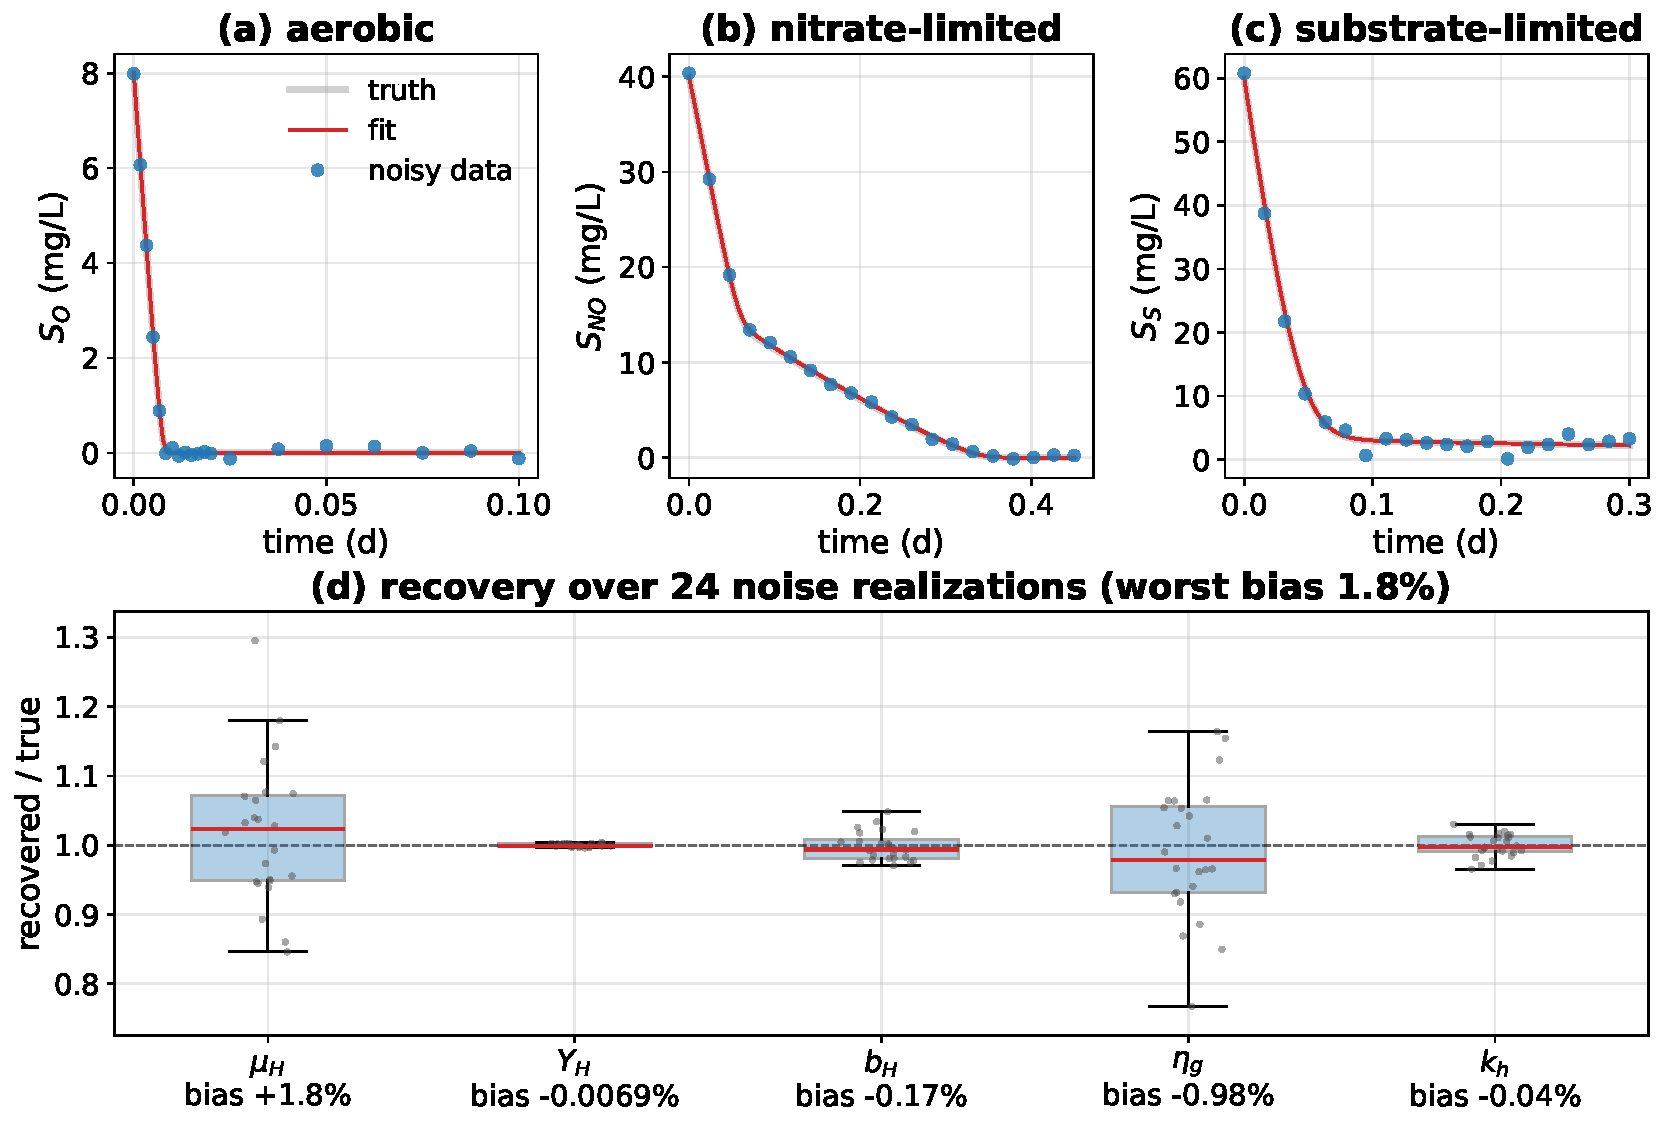
\includegraphics[width=\linewidth]{fig_calibration}
  \caption{Multi-parameter calibration of activated-sludge kinetics from noisy batch
  assays. (a)--(c) Three closed-batch assays of the same reactor, differing only in
  initial state, each showing the noisy observations, the fitted trajectory and the
  true trajectory of the diagnostic species (dissolved oxygen for the aerobic
  respirogram, nitrate and substrate for the anoxic assays). (d) The
  \CalNfree\ recovered parameters over \CalNmc\ independent noise realizations, each
  fitted without priors from its own random start (Section~\ref{sec:methods-calibstudy}),
  normalized to its true value; every bias is within its Monte Carlo standard error,
  the largest \CalWorstBias\,\% in \CalWorstBiasName.}
  \label{fig:calibration}
\end{figure}

The same exact sensitivities give the Fisher information of a design before any data are collected. Evaluated at the true parameter values, \(\boldsymbol{\mathcal{I}}\) (Eq.~\eqref{eq:fisher}) needs one sensitivity solve per assay and no fit, and its eigen-directions say which combinations of the parameters the data determine: each eigenvector names a combination by its loadings, and its eigenvalue \(\lambda\) sets the Cram\'er--Rao standard deviation \(1/\sqrt{\lambda}\) with which the data determine it. On this design the weakest direction is the same with and without the aerobic assay (Figure~\ref{fig:identifiability}b). It loads \IdentWeakLoadMu\ on \(\log\mu_H\) and \IdentWeakLoadEtag\ on \(\operatorname{logit}\eta_g\), a ratio of \IdentWeakLoadRatio. Since a change \(\delta\) in \(\operatorname{logit}\eta_g\) changes \(\log\eta_g\) by \((1-\eta_g)\,\delta\), and \(1-\eta_g=\IdentOneMinusEtag\) at the true value, this is exactly the direction along which the product \(\eta_g\mu_H\) stays fixed. Anoxic growth runs at that product, so anoxic data cannot move along this direction, and only the aerobic respirogram, where growth runs at \(\mu_H\) alone, constrains it.

The eigenvalue of that direction distinguishes two kinds of non-identifiability. In the full design it is small but not zero, \IdentWeakRelFull\ of the largest: a practical non-identifiability, with Cram\'er--Rao relative standard deviations of \IdentCrbMuFull\,\% for \(\mu_H\) and \IdentCrbEtagFull\,\% for \(\eta_g\), far above those of the other three parameters. These are the design-stage predictions of the spreads in Figure~\ref{fig:calibration}, and both the Laplace intervals of the individual fits (\CalPredCVmu\ and \CalPredCVetag\,\%) and the realized Monte Carlo spread (\CalEmpCVmu\ and \CalEmpCVetag\,\%) agree with them. Without the aerobic assay, the eigenvalue falls to round-off, \IdentWeakRelAnox\ of the largest, and the condition number rises from \IdentKappaFull\ to \IdentKappaAnox, beyond the reciprocal of double-precision machine epsilon (Figure~\ref{fig:identifiability}a). That is a structural non-identifiability: \(\mu_H\) and \(\eta_g\) have infinite Cram\'er--Rao standard deviations, and their correlation reaches \IdentCorrAnox\ (\IdentCorrFull\ in the full design). A recovery from perturbed starts shows the consequence (Figure~\ref{fig:identifiability}c). Under the anoxic-only design the estimates of \(\mu_H\) and \(\eta_g\) slide along the constant-product ridge, scattering by \IdentMuCVanox\ and \IdentEtagCVanox\,\% while their product stays within \IdentProductCVanox\,\%. Under the full design they lie on the same ridge but are held close to the truth. This \(\mu_H\)--\(\eta_g\) coupling is a known structural non-identifiability of the activated-sludge models \citep{vanrolleghem1995}. The result here is not its discovery but a demonstration that the exact Fisher information recovers it, together with the reason. This same process can be applied to any kinetic model to determine its identifiability.

\begin{figure}[htbp]
  \centering
  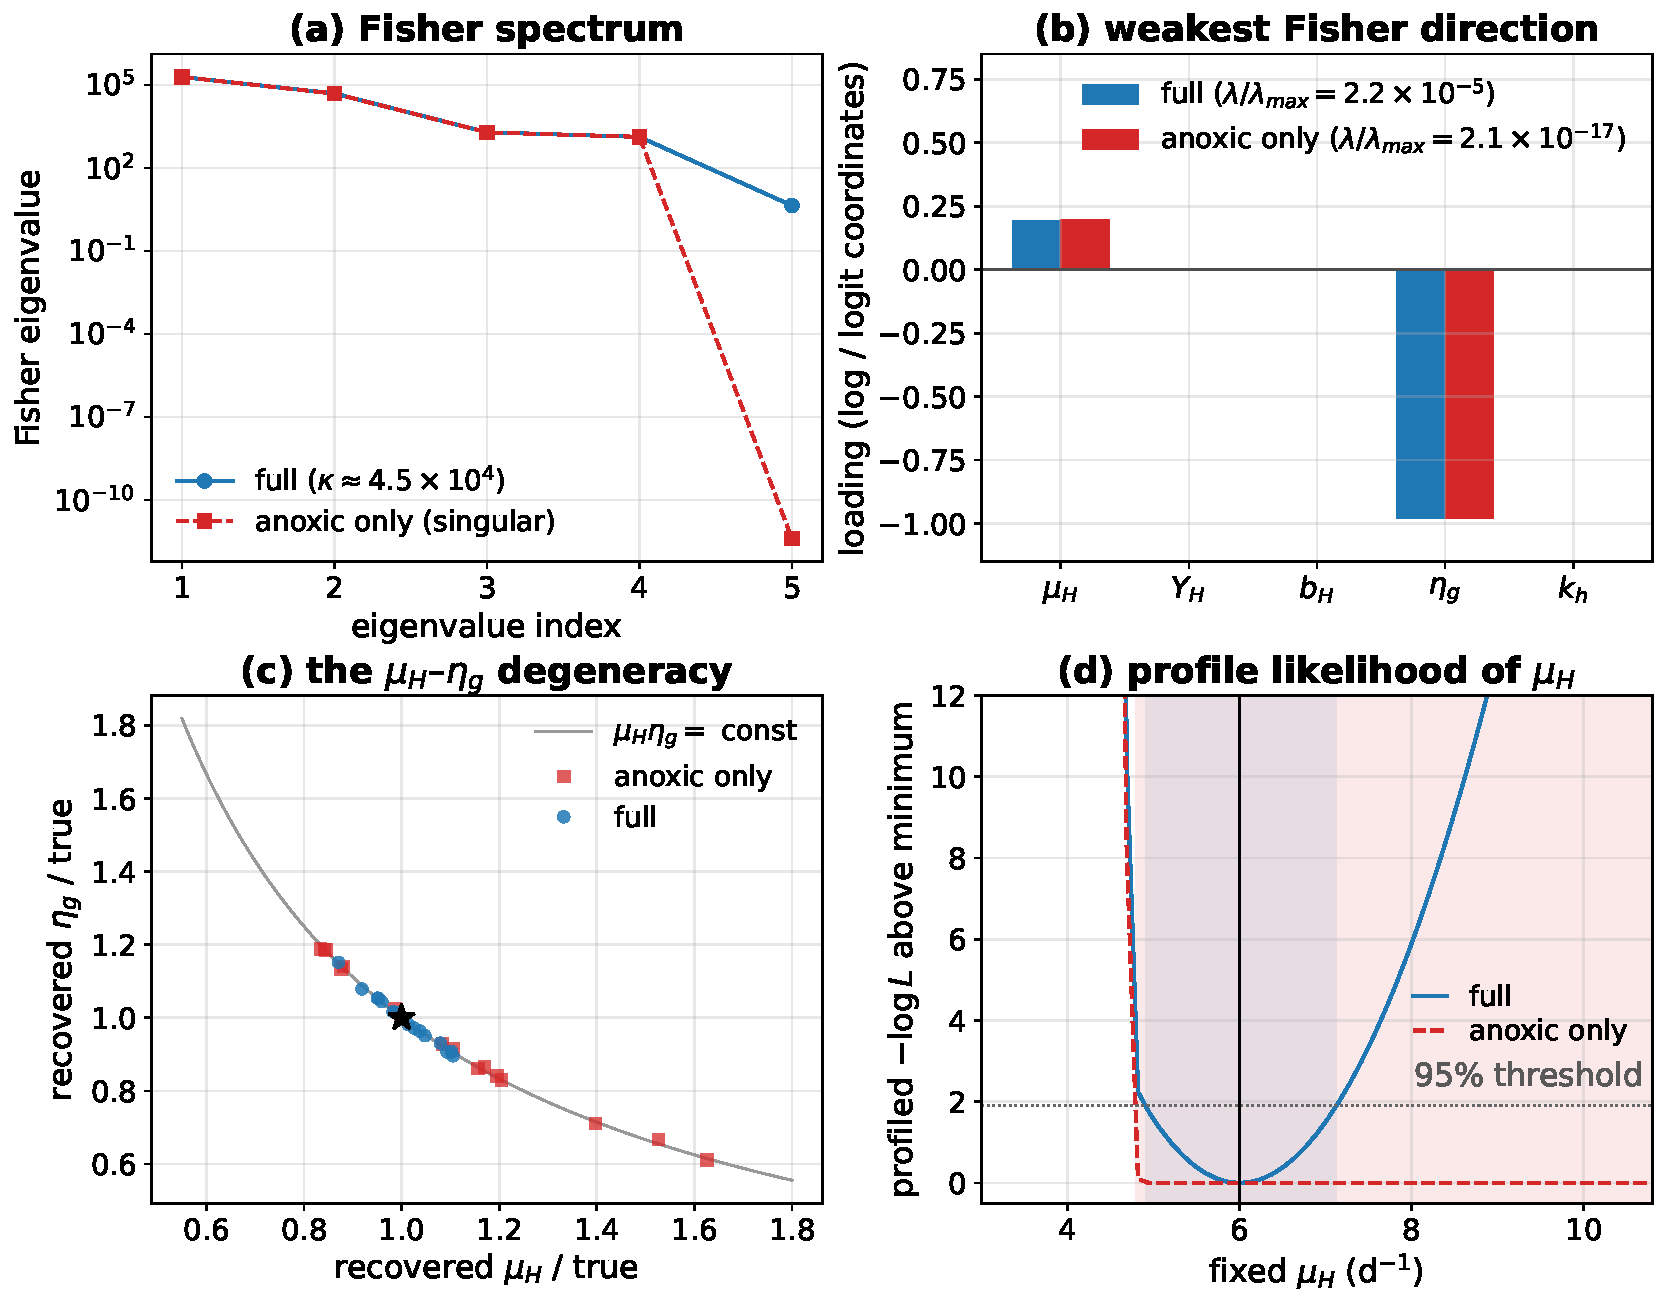
\includegraphics[width=\linewidth]{fig_identifiability}
  \caption{Practical identifiability read from the exact Fisher information,
  evaluated at the true values before any fit, for the heterotroph parameters under
  two experimental designs: the full three-assay set and the two anoxic assays alone.
  (a) The Fisher eigenvalue spectrum. Dropping the aerobic respirogram turns the
  weakest direction from weak into null: its eigenvalue falls to round-off and the
  condition number jumps from \IdentKappaFull\ to \IdentKappaAnox, so the matrix is
  numerically singular. (b) The loadings of the weakest direction in each design
  (log and logit coordinates; \(\lambda/\lambda_{\max}\) in the legend): the same
  combination of \(\mu_H\) and \(\eta_g\), the one that keeps their product fixed.
  (c) Recovery over \IdentNmc\ noise realizations, each fitted without priors from a
  random start (Section~\ref{sec:methods-calibstudy}): under the
  full design the estimates stay close to the truth (star) along the same ridge, while under the anoxic-only
  design \(\mu_H\) and \(\eta_g\) slide along the constant-product ridge
  (\(\mu_H\eta_g=\)~const), individually lost but jointly determined. (d) Profile
  likelihood of \(\mu_H\): at each fixed \(\mu_H\) the other parameters are
  re-optimized and the negative log-likelihood is shown relative to its minimum. The
  dotted line is the \(95\%\) likelihood-ratio threshold, the shaded bands are the
  resulting intervals, and the vertical line is the true value. The full design gives
  a well-defined minimum, while the anoxic-only profile stays flat as \(\eta_g\)
  compensates, rising only where \(\eta_g\) reaches its physical bound.}
  \label{fig:identifiability}
\end{figure}

Because the measurements from each experiment are independent, the information of a combined design is the sum of the information of its assays, \(\boldsymbol{\mathcal{I}}_{\mathrm{full}}=\boldsymbol{\mathcal{I}}_{\mathrm{aerobic}}+\boldsymbol{\mathcal{I}}_{\mathrm{anoxic}}\), which here holds to a relative difference of \IdentAdditivity. The aerobic respirogram on its own is a poor design, leaving \(\mu_H\) uncertain by \IdentCrbMuAer\,\% and \(b_H\) by \IdentCrbBhAer\,\%, but its information lies along the anoxic pair's null direction, so together they determine all five parameters. Ranking the possible additions to the anoxic pair by the D-criterion \(\Phi_D=\log\det\boldsymbol{\mathcal{I}}\) (Eq.~\eqref{eq:dcrit}) states the design rule directly: adding the aerobic respirogram gives a finite criterion, while repeating either anoxic assay leaves it at \(-\infty\) however often it is repeated, because more of the same data adds information only along directions that are already determined. An aerobic assay must accompany anoxic data if the growth rate and the anoxic factor are to be told apart. A profile likelihood confirms this beyond the local Fisher approximation. Fixing \(\mu_H\) across a grid and re-optimizing the other parameters, the full design constrains \(\mu_H\) to a \(95\%\) likelihood-ratio interval of \IdentProfLoFull--\IdentProfHiFull~d\(^{-1}\) around the true \IdentMuHTrue~d\(^{-1}\) (Figure~\ref{fig:identifiability}d). Its lower end lies close to \(\eta_g\mu_H=\IdentProdTrue\)~d\(^{-1}\), where \(\eta_g\) reaches its logit bound of one, so it is set partly by that bound rather than by the data alone. Under the anoxic-only design the profiled objective stays flat from \IdentProfLoAnox~d\(^{-1}\) to the upper end of the profiled range at \IdentProfGridHi~d\(^{-1}\), so the data set no upper limit on \(\mu_H\) at all: \(\eta_g\) slides to hold the product fixed, and the lower end is again where \(\eta_g\) reaches its bound. The near-null direction the Fisher spectrum flags is therefore not an artifact of the quadratic approximation.

The same gradients also improve a design. With the two anoxic assays fixed, the engine's experiment-design routine moves the \DesignNsamp\ sampling times of the aerobic respirogram, at least \DesignSpacingMin~min apart within its \DesignTaerMin-min run, and its initial substrate within \DesignSSLo--\DesignSSHi~mg~COD/L, to maximize the D-criterion of the whole design. The criterion is differentiated with respect to the design itself, through the Fisher information and the stiff solves. The optimum (Figure~\ref{fig:design}a) clusters the samples into an early group at \DesignEarlyLo--\DesignEarlyHi~min, while the dissolved oxygen is falling, and a later one at \DesignLateLo--\DesignLateHi~min, and puts the initial substrate at its upper bound of \DesignSSOpt~mg~COD/L. It raises \(\log\det\boldsymbol{\mathcal{I}}\) from \DesignDBase\ to \DesignDOpt, a factor of \DesignDetFactor\ in \(\det\boldsymbol{\mathcal{I}}\), and lowers the predicted relative standard deviations of \(\mu_H\) from \DesignCrbMuBase\ to \DesignCrbMuOpt\,\% and of \(\eta_g\) from \DesignCrbEtagBase\ to \DesignCrbEtagOpt\,\%, leaving the other three unchanged (Figure~\ref{fig:design}b). Blind recoveries on the designed experiment, \DesignNmc\ noise realizations with the scheme of Figure~\ref{fig:calibration}, realize \DesignEmpMuOpt\ and \DesignEmpEtagOpt\,\% against \CalEmpCVmu\ and \CalEmpCVetag\,\% on the original design, so the predicted gain is realized. Like any locally optimal design, this one is computed at assumed parameter values and trusts the model between its sample clusters, so in practice a few samples between the clusters guard against model error.

\begin{figure}[htbp]
  \centering
  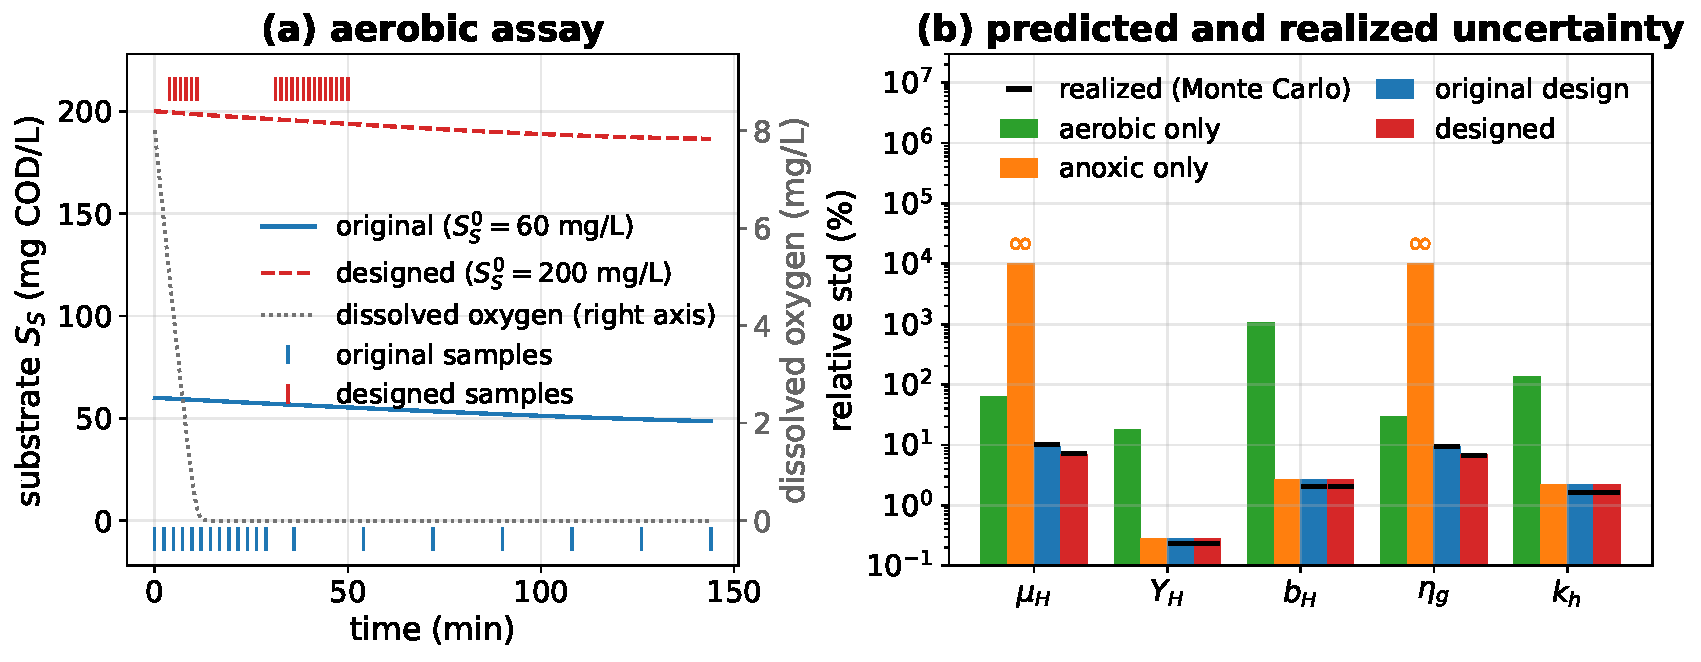
\includegraphics[width=\linewidth]{fig_design}
  \caption{Gradient-based design of the calibration experiment. With the two anoxic
  assays fixed, the D-criterion of the three-assay design is maximized over the
  aerobic respirogram's \DesignNsamp\ sampling times and its initial substrate.
  (a) The observed substrate \(S_S\) of the aerobic assay at the original
  (\DesignSSBase~mg~COD/L) and designed (\DesignSSOpt~mg~COD/L) initial substrate,
  with the dissolved oxygen (dotted, right axis) and the original (bottom) and
  designed (top) sampling times. (b) Cram\'er--Rao relative standard deviation of
  each parameter for the aerobic assay alone, the anoxic assays alone (\(\infty\):
  structurally non-identifiable), the original three-assay design and the designed
  one, with the realized spread of \DesignNmc\ blind Monte Carlo recoveries (black
  bars) on the original and the designed experiment.}
  \label{fig:design}
\end{figure}

The twin experiments establish the estimator's behaviour on data the model itself generated. We close by taking the same exact gradients to real measurements, to test whether they discriminate competing kinetic structures and read the identifiability of each outside the twin-experiment setting. Applying the estimator to the \RespNww\ real respirograms of Section~\ref{sec:methods-calibstudy}, we compare two heterotroph structures, a reduced ASM1 growth core and a modified ASM3 storage structure, swapped by editing the model file and nothing else (Figure~\ref{fig:respirometry}). Both hold the biomass and the half-saturation fixed, since \(\mu_H\) is identifiable from a single respirogram only then: growth enters the uptake through the product \(\mu_H X_H\), and \(K_S\) trades off against \(\mu_H\) along the substrate curve.

\begin{figure}[htbp]
  \centering
  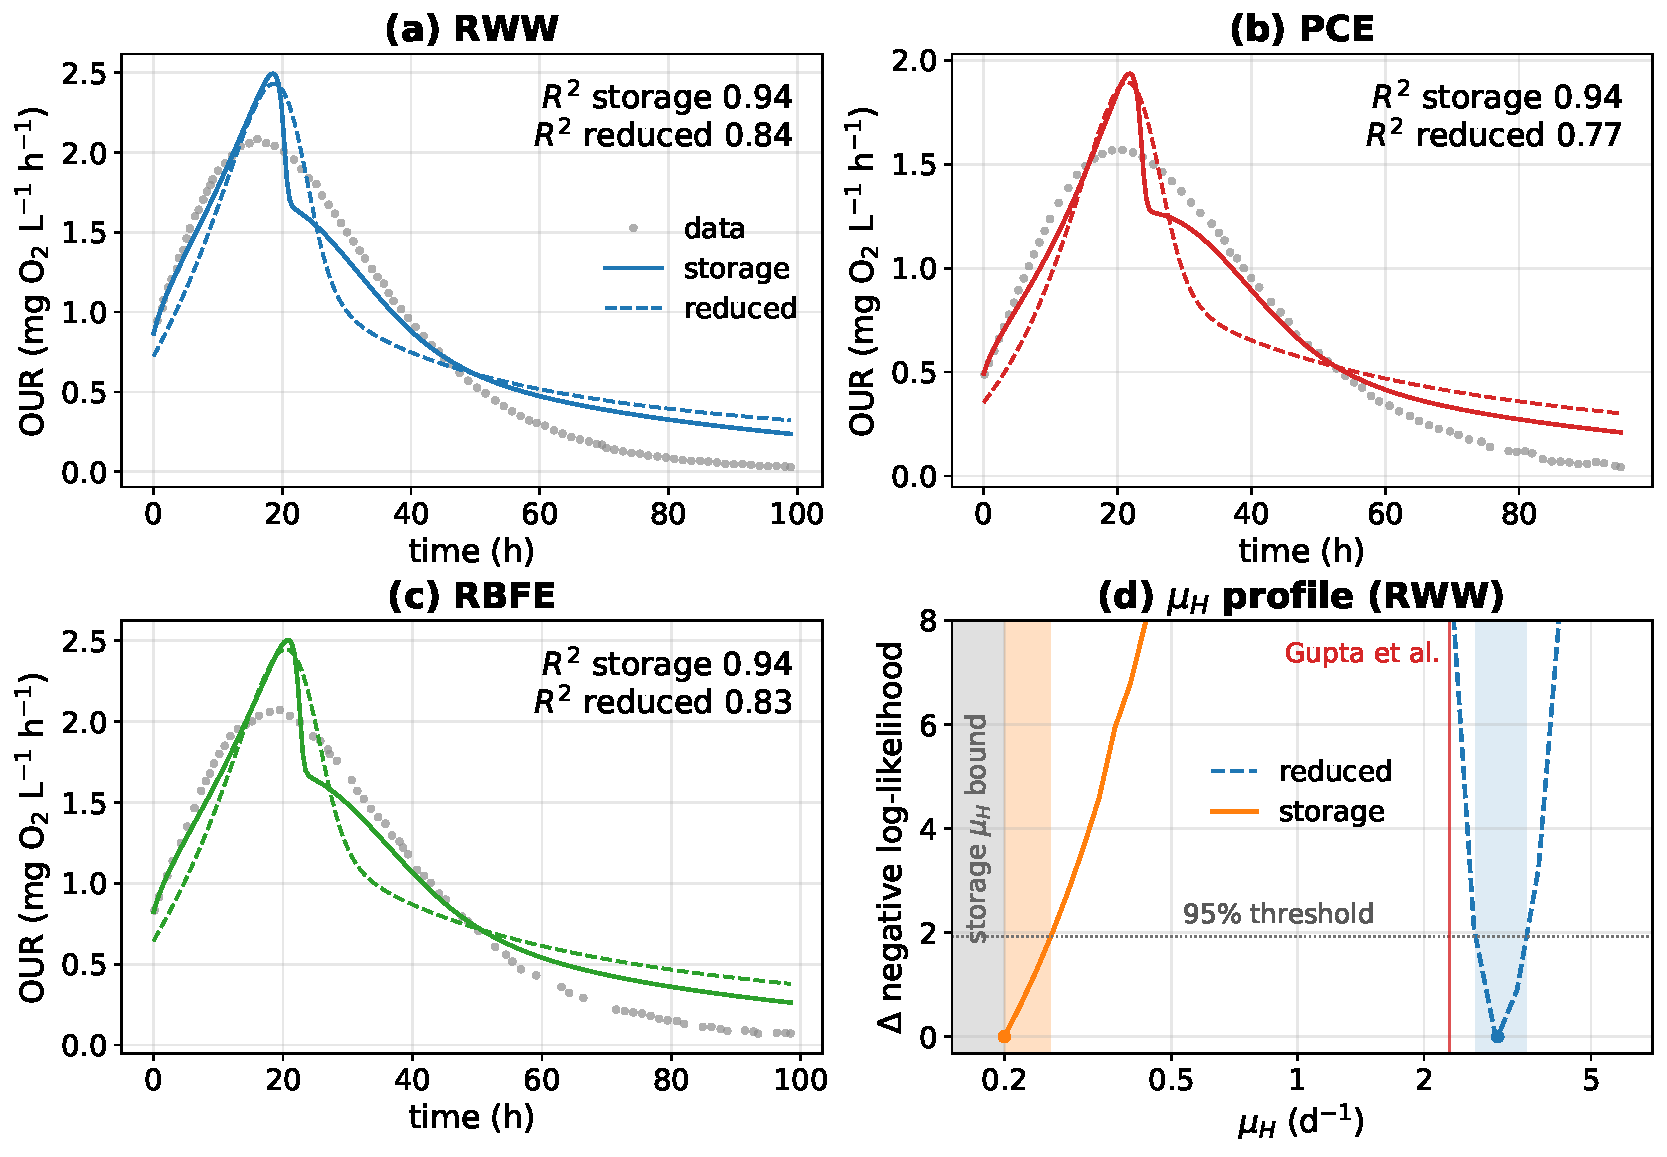
\includegraphics[width=\linewidth]{fig_respirometry}
  \caption{Real-data comparison of two heterotroph model structures, swapped by
  editing the YAML file, calibrated to aerobic respirograms of three filtered
  municipal wastewaters, digitized from Figure~4-1 of \citet{gupta2018thesis}. (a)--(c) Digitized oxygen-uptake-rate (OUR) data
  (points) with the storage model (modified ASM3, simultaneous storage and growth;
  solid) and the reduced model (ASM1 with death regeneration; dashed); the
  \(R^2\) of each model is inset. Both structures overshoot the peak; the storage
  model follows the falling limb (\(R^2=\RespStRtwo\)), while the reduced model
  falls below it and leaves a larger residual. In both, the biomass \(X_H\) is held at
  the value reported by the source study and the half-saturation \(K_S\) at a
  standard literature value. (d) Profile likelihood of \(\mu_H\) for the
  \RespProfileWW\ respirogram: the negative log-likelihood, re-minimized over the
  other free parameters at each fixed \(\mu_H\) with the noise level fixed at the
  best-fit residual, above its minimum, on a logarithmic \(\mu_H\) axis, with the 95\%
  threshold (dotted). The shaded bands are each model's 95\% interval, the dots its
  best fit, and the grey region lies below the storage model's lower bound on
  \(\mu_H\). Under the
  reduced model \(\mu_H\) has a sharp minimum (95\% interval
  \RespProfLoDr--\RespProfHiDr~d\(^{-1}\)), above the source study's value (red
  line); under the storage model the data drive \(\mu_H\) to its lower bound. It is
  identifiable in one structure, not the other.}
  \label{fig:respirometry}
\end{figure}

The claim on real data is a model-discrimination claim, not a predictive validation. The point is that the same exact gradients that fixed the identifiability geometry on model-generated data now, on measured wastewater, tell two competing kinetic structures apart and read the identifiability of each, through a single edit of the model file. A predictive validation is a separate task, out of scope here and in any case unavailable from these data, since the respirograms are digitized and the reported parameters come from a different estimator on the same curves. As a first check that the fits are sensible, the reduced model's whole-curve \(\mu_H\) can be set beside the value the source study obtained by its graphical rise-slope method. It is \(\RespMuFitRWW\), \(\RespMuFitPCE\) and \(\RespMuFitRBFE\)~d\(^{-1}\), with Laplace standard deviations of \RespDrMuStdLo--\RespDrMuStdHi~d\(^{-1}\), against \(\RespMuRepRWW\), \(\RespMuRepPCE\) and \(\RespMuRepRBFE\)~d\(^{-1}\), so it is \RespDrErrBest--\RespDrErrWorst\,\% higher. It places the primary-clarifier effluent highest, as the source study does, but cannot separate the other two, which lie within one standard deviation of each other. The two estimators answer different questions. The graphical method reads the initial-phase slope with the reported COD fractionation imposed, while the whole-curve fit uses the entire transient and also estimates the initial pools, whose total it places at \RespCodRatioLo--\RespCodRatioHi\ of the reported COD. Their comparison is therefore a consistency check between two estimators of a structure-dependent quantity, not an accuracy claim (the graphical analysis represents readily biodegradable substrate as a constant-uptake plateau, which, propagated through the dynamic model, gives a \RespGuptaOverLo--\RespGuptaOverHi\(\times\) higher modelled peak, a difference of representation, not of correctness). Following respirometric practice, goodness of fit is reported as the root-mean-square error (RMSE) of the oxygen uptake rate, with \(R^2\) alongside, since \(R^2\) on a smooth uptake curve is an insensitive measure of fit. Neither structure reproduces the whole curve, and that is a property of the activated-sludge kinetics being fitted rather than of the estimator. Both overshoot the peak and run above the data in the late tail, and the reduced model also falls below the data on the falling limb after the peak (RMSE \RespDrRmseLo--\RespDrRmseHi~mg~O\(_2\)~L\(^{-1}\)~h\(^{-1}\), \(R^2=\RespDrRtwoLo\text{--}\RespDrRtwoHi\)), the famine-phase misfit that growth-only activated-sludge structures are known to show on real respirograms \citep{guisasola2005}.

Editing the model to the storage structure closes most of the falling-limb discrepancy and lowers the misfit on every wastewater (RMSE \RespStRmseLo--\RespStRmseHi~mg~O\(_2\)~L\(^{-1}\)~h\(^{-1}\), \(R^2=\RespStRtwo\) on all three), though the peak overshoot and the late-tail excess remain. The cost of the added pathway is identifiability, and the exact-gradient profile likelihood reads it off directly (Figure~\ref{fig:respirometry}d). Under the reduced structure the uptake is attributed to direct growth and the \(\mu_H\) profile has a sharp minimum, with a 95\% profile-likelihood interval of \RespProfLoDr--\RespProfHiDr~d\(^{-1}\). The source study's value lies outside it, \RespProfRepRise\ above the minimum in negative log-likelihood, consistent with the two estimators holding different quantities fixed. Under the storage structure the data attribute the uptake to storage: the direct-growth \(\mu_H\) profile rises steeply from its lower bound of \RespStMuBound~d\(^{-1}\), with a 95\% interval that runs from the bound to \RespProfHiSt~d\(^{-1}\), so \(\mu_H\) is no longer separately recoverable. This is the known result that storage kinetics require dedicated storage measurements \citep{guisasola2005}, here read off a real respirogram by the gradient. Which parameters a measurement can constrain is thus contingent on the assumed structure, the same identifiability lesson as the twin experiments, now on real data. The single-parameter, noise-free recovery that isolates gradient correctness is reported in the supplementary material (Section~\ref{si:single-param}).

\subsection{Performance}
\label{sec:results-performance}

The cost of the engine is dominated by the one-time compilation of the plant right-hand side. The first solve of the BSM1 plant, which compiles the \PerfNstate-state right-hand side (the thirteen activated-sludge states in each of the five reactors) and integrates it over the fourteen-day dry-weather dynamic horizon, takes \PerfCompileS~s. Once compiled, the program is reused, and a subsequent solve of that same fourteen-day run with changed parameters takes \PerfSolveS~s. Changing a parameter value does not retrigger compilation, since the parameters enter as data rather than as part of the compiled function. Editing the model structure does retrigger it, because the compiled right-hand side then changes. Adding a species, changing a rate law, or swapping the model pays the compile again. A calibration or a parameter sweep over a fixed structure does not. A reverse-mode gradient of a scalar plant loss with respect to the parameter vector costs \PerfADFactor\ times a single solve, independent of the \PerfNparams\ parameters differentiated against. A finite-difference gradient of the same loss would cost \PerfFDFactor\ solves, one per parameter plus the base point, so the exact gradient is already cheaper at this parameter count and its advantage grows with the number of parameters, as measured for the calibration objective in Figure~\ref{fig:adfd}b. Figure~\ref{fig:performance}a shows the compilation, solve, and gradient costs.

The value of the exact gradient over finite differencing is cost and robustness rather than single-fit accuracy. On the batch calibration objective of Section~\ref{sec:results-diff}, where a central finite difference costs two solves per parameter, the measured cost per gradient is flat for the exact gradient and linear for finite differences, a measured factor of \AdfdRatio$\times$ at \CalNfree\ parameters (Figure~\ref{fig:adfd}b) and, extrapolating the finite-difference line's measured slope, \AdfdProj$\times$ at the roughly twenty kinetic parameters of a full activated-sludge calibration. Finite differencing also needs a step size. Its error is truncation-limited at large steps and solver-noise-limited at small steps, with a floor of $\AdfdFloor$ on this well-resolved batch (Figure~\ref{fig:adfd}a), whereas the exact gradient needs no step and carries only the solver tolerance. That floor is set by the accuracy of the solve and rises with its stiffness and length. On the full open-loop BSM1 plant, whose recycle-coupled solve is longer and stiffer than the batch, the same finite-difference floor is about \AdfdFloorRatio\ times higher at $\AdfdPlantFloor$ (Figure~\ref{fig:adfd}a), while the exact adjoint carries only the solver tolerance in either case. The advantage of exact differentiation therefore grows as the model does.

\begin{figure}[htbp]
  \centering
  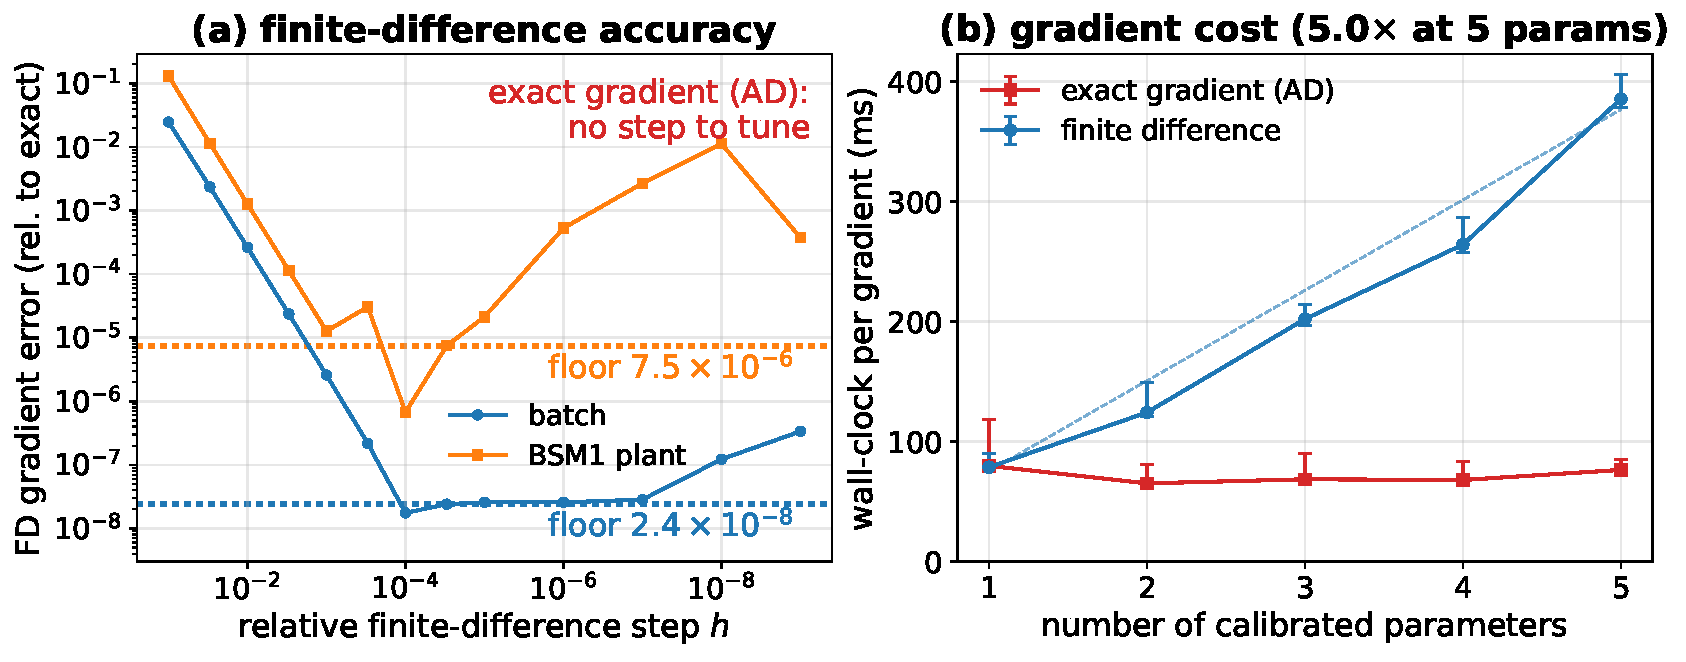
\includegraphics[width=\linewidth]{fig_ad_vs_fd}
  \caption{Exact gradients against finite differences on the calibration objective.
  (a) The finite-difference gradient error against step size, for the batch
  calibration loss and for a calibration loss on the full open-loop BSM1 plant. Both
  are truncation-limited at large steps and floored by solver noise at small steps;
  the plant floor is higher because its recycle-coupled solve is stiffer and longer,
  while the exact gradient needs no step in either case. (b) The measured wall-clock
  per gradient against the number of calibrated parameters; the exact reverse-mode
  gradient is one adjoint pass and is flat, while finite differencing costs two solves
  per parameter and grows linearly. Points are the median over \AdfdNrep\ timed trials,
  interleaved across the parameter counts, and the 10th--90th-percentile bars lie
  within the markers.}
  \label{fig:adfd}
\end{figure}

The cost also scales gracefully with the size of the model. Compiling and solving a family of synthetic first-order chains of growing species count, which isolates the engine's cost from any single model's chemistry, the amortized solve grows sub-quadratically, as \(N^{\PerfScaleSolveExp}\) in the state dimension \(N\) over \PerfScaleNmin--\PerfScaleNmax\ species, while the one-time compilation is nearly flat at \(N^{\PerfScaleCompileExp}\) (Figure~\ref{fig:performance}b). The two costs have different origins. Compilation parses the rate syntax trees and lowers a single vectorized kernel whose graph grows slowly with the model, whereas the solve is dominated by the per-step implicit linear algebra on the state vector. For the assembled plant, whose Jacobian is block-sparse, that per-step linear algebra forms the Jacobian by column-compressed (graph-colored) automatic differentiation, evaluating it in a number of tangent passes set by the widest coupled unit block rather than the full state dimension. The activated-sludge and anaerobic-digestion models used here sit at the small end of this range. First-order chains are a benign, sparsely coupled family, so the measured exponents isolate the engine's own overhead and are a lower bound. A dense, stiff biokinetic model with shared saturation terms may scale less favourably, and the exponents should be read as the engine's cost, not a guarantee for every model.

The reported solve and gradient times are medians over \PerfNruns\ runs of the already-compiled program, and the per-size solve times behind the scaling fit are medians over \PerfScaleNruns\ runs. The compilation is the one-time first-call cost. These timings are reported on a single machine and are indicative. The relative costs and the scaling exponents are the portable quantities.

\begin{figure}[htbp]
  \centering
  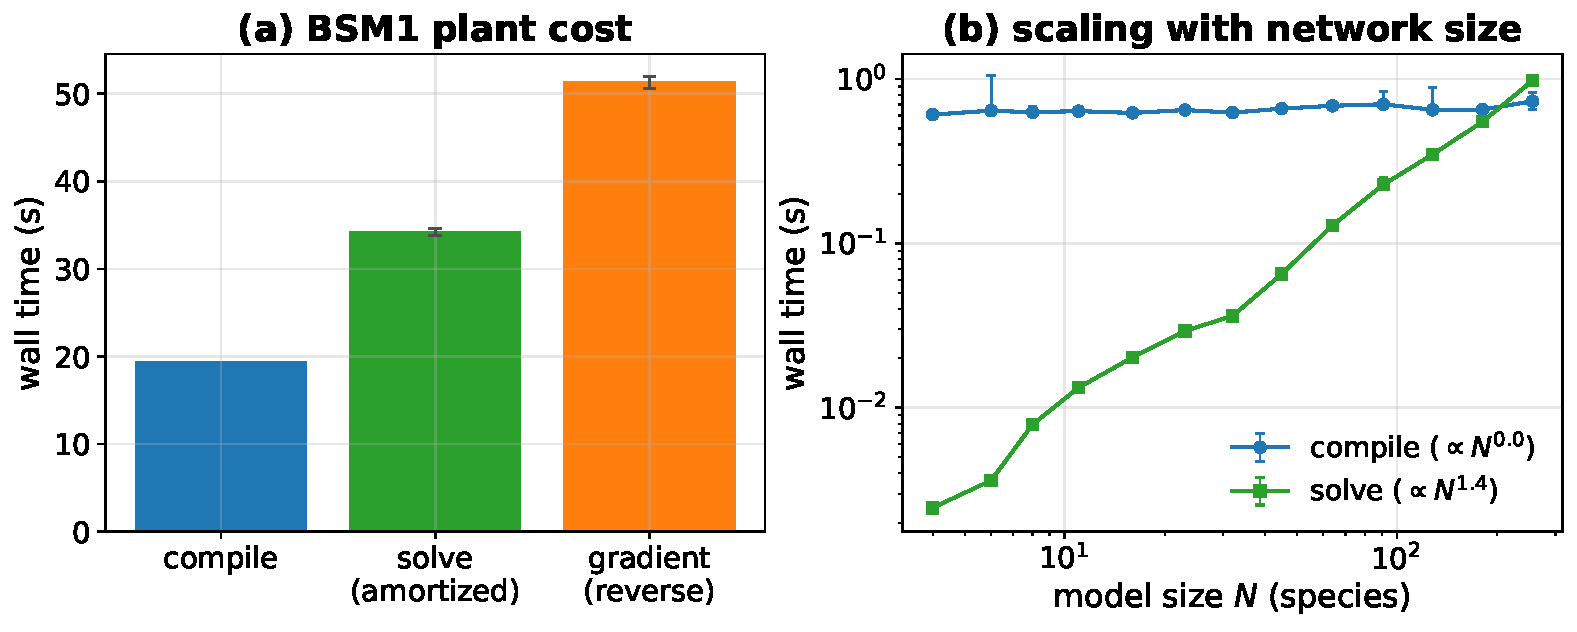
\includegraphics[width=\linewidth]{fig_performance}
  \caption{Cost of the engine. (a) The BSM1 plant: the one-time compilation of the
  right-hand side, an amortized solve with changed parameters, and a reverse-mode
  gradient; the solve and gradient bars are the median over \PerfNruns\ timed runs with a
  10th--90th-percentile error band, while the compilation is a single one-time event.
  The compilation dominates and is amortized across repeated solves by the
  compiled-solve cache, and the gradient-cost scaling with parameter count is measured
  in Figure~\ref{fig:adfd}b. (b) Scaling with model size, measured on synthetic
  first-order chains of growing species count \(N\) on log axes: the amortized solve
  grows sub-quadratically as \(N^{\PerfScaleSolveExp}\) and the one-time compilation is
  nearly flat at \(N^{\PerfScaleCompileExp}\).}
  \label{fig:performance}
\end{figure}

% =========================================================================
\section{Discussion}
\label{sec:discussion}

The engine resolves the tension set out in the introduction. A reaction model is declared as data and changed at run time, yet its rate laws are evaluated safely, without executing text as code, and the evaluation is differentiable and compiled for speed. The construction that achieves this is the parse of each rate law into an abstract syntax tree and the mapping of that tree onto elementary differentiable operations. The tree is the single representation that is at once human-readable in the source file, safe because only declared names and a fixed function set can appear, open to inspection and to checks such as the conservation audit, and differentiable because each node has a known derivative. Hard-coding, direct evaluation of the text, and per-model code generation each give up one of these properties.

The benchmark reproduction establishes that the differentiability is not bought at the cost of correctness. The assembled BSM1 plant reproduces the published benchmark at steady state across every reactor and the settler, with a worst relative difference of \SteadyReactorWorstPct\,\%, and reproduces the dry-weather flow-weighted effluent averages and the quality indices with a largest difference of \DynEffWorstPct\,\%. This is numerical equivalence with a reference implementation rather than an independent validation of model fidelity, but it is the property a gradient depends on. A gradient is only as meaningful as the model it differentiates, and here that model is shown to be the benchmark's, reproduced exactly. The verification against a closed-form solution and against finite differences then confirms that the gradient the engine returns is the exact gradient of that model.

The quantitative evidence in this paper is of two kinds, and this is stated plainly. The BSM1 results are numerical equivalence against the benchmark's own reference implementation. The calibration and identifiability results are twin experiments, in which the model generates the data that are then fit back. The single real-data study is a qualitative model-structure comparison, with no independent ground truth. None of these is an independent predictive validation against measured plant data. That validation is a separate task, out of scope here, where the aim is the engine and the correctness of its gradients.

The capability the gradients provide is the reason to build the engine. The calibration and sensitivity demonstration is deliberately small, but it shows the shape of what the gradients enable. Calibration becomes optimization with an exact gradient rather than a derivative-free search, and sensitivity becomes a direct derivative rather than a finite-difference sweep. The advantage is structural. The reverse-mode gradient returns the sensitivity to all parameters at once, so the cost of a full sensitivity or of a gradient step does not grow with the number of parameters, which is the regime where derivative-free and finite-difference methods become expensive.

The engine is not specific to the activated sludge models used for most of the demonstrations here. The model format, parser, and differentiable evaluation are generic, and the anaerobic digester already draws on the parts of the expression language that the activated-sludge models leave idle. Its rate laws are gated by the pH-dependent switching and inhibition functions of Section~\ref{sec:methods-parser}, evaluated at a pH that is itself state-derived through the differentiable charge-balance speciation (Section~\ref{sec:methods-conditions}), so acid/base equilibrium chemistry is exercised and differentiated in a genuine result. The same functions, format, and evaluator carry over unchanged to the kinetic schemes of water chemistry, which a user declares in the same plain-text form, and the plant composition applies to any flowsheet of reacting and non-reacting units. We validate the engine here on the wastewater benchmarks rather than on the range of chemistries the format admits. The scope of this paper is the engine and its correctness.

% =========================================================================
\section{Conclusions}
\label{sec:conclusions}

\texttt{aquakin} is an open-source engine that makes a reaction model both reconfigurable at run time and differentiable from end to end. A model is declared as data, each rate law is parsed into an abstract syntax tree and compiled through JAX into a safe, just-in-time, differentiable function, and unit operations compose into a plant whose entire flowsheet is one differentiable program. The engine reproduces the open-loop BSM1 benchmark at steady state and in the dry-weather flow-weighted effluent averages. Its gradients, formed by the discrete adjoint the calibration relies on, match a closed-form derivative to solver tolerance on both a non-stiff and a stiff problem, and a finite-difference gradient through the assembled plant to the finite-difference floor. Those gradients turn calibration and sensitivity analysis into direct computations. The calibration and identifiability results are established in twin experiments on model-generated data, with a real-data respirometric demonstration that the same gradients discriminate model structures and expose the structure-dependence of what a measurement identifies. The measured cost scaling is reported for the models studied and should be read as indicative rather than as a guarantee for arbitrarily dense stiff models. By combining run-time configurability with exact differentiability in a safe and introspectable form, the engine brings to wastewater-treatment modelling the gradient-based capabilities that have advanced neighbouring computational fields, principally for research on calibration, identifiability, and experimental design rather than, yet, for production plant modelling in place of the established simulators.

% =========================================================================
\section*{Software and data availability}
\begin{description}
\setlength{\itemsep}{0pt}
\item[Name] \texttt{aquakin}.
\item[Developer and contact] C.~T.~DeGroot (christopher.degroot@uwo.ca).
\item[Year first available] 2026.
\item[Hardware required] any 64-bit platform that runs Python; no special hardware, with optional GPU or TPU acceleration through JAX.
\item[Software required] Python 3.11 or newer (as JAX 0.10 requires), with JAX and jaxlib, Diffrax, Optimistix, Pydantic, PyYAML, NumPy and SciPy.
\item[Program language] Python.
\item[Program size] about 43\,000 lines across 117 Python modules.
\item[Availability and cost] open-source under the MIT license, free of charge, at \url{https://github.com/DeGrootResearchGroup/aquakin} (version~0.1.0). A tagged release archived under a permanent DOI (Zenodo) will be cited in the final version.
\end{description}

The data used for validation, the published open-loop BSM1 reference values, the ASM1 parameter set and the dry-weather influent, are provided as JSON and CSV files (about 120\,kB) in the paper repository, which also holds the figure and table generation scripts and rebuilds every number, figure and table in this paper from the code.

\section*{Declaration of competing interests}
The author delares no competing interests.

\section*{Funding sources}
This work was supported by the Natural Sciences and Engineering Research Council of Canada [RGPIN-2024-05703].

\section*{Acknowledgements}
The BSM1 implementation and reference results were provided by the Department of Industrial Electrical Engineering and Automation, Lund University (U. Jeppsson, C. Rosen).

\section*{Declaration of generative AI and AI-assisted technologies in the manuscript preparation process.}
During the preparation of this work the author used Anthropic's Claude models (primarily Opus 4.8 and Opus 5.5) to write/edit code and prose. After using these tools, the author reviewed and edited the content as needed and takes full responsibility for the content of the published article.

% =========================================================================
\bibliographystyle{plainnat}
\bibliography{references}

% =========================================================================
\newpage
\appendix

% --- Supplementary numbering: sections, equations, figures, and tables
%     restart at 1 with an ``S.'' prefix (S.1, S.2, ...), independent of
%     the body. ---
\setcounter{section}{0}
\setcounter{equation}{0}
\setcounter{figure}{0}
\setcounter{table}{0}
\renewcommand{\thesection}{S.\arabic{section}}
\renewcommand{\theequation}{S.\arabic{equation}}
\renewcommand{\thefigure}{S.\arabic{figure}}
\renewcommand{\thetable}{S.\arabic{table}}

% =========================================================================
\begin{center}\large\bfseries Supplementary Material\end{center}
% =========================================================================

\section{Numerical settings}
\label{si:settings}
Unless Table~\ref{tab:settings} says otherwise, every solve uses the engine's default configuration: an ESDIRK Kvaerno method with a PID adaptive step-size controller, a relative tolerance \(\mathrm{rtol}=10^{-6}\), an absolute tolerance that auto-scales per component to \(10^{-6}\) of the component's magnitude, and no step-size limitation. The step-size controller is a non-differentiated control. It selects the steps on the forward pass, and the reverse pass differentiates the resulting fixed sequence of implicit steps, each solved to the root-finder tolerance, so the returned gradient is the exact gradient of that discrete trajectory. Times are in the model's native unit (days for the activated-sludge and digester models).

The reverse-mode gradient of the coupled plant, including the plant leg of the forward-versus-reverse check in Section~\ref{sec:results-verification-fd}, uses the discrete adjoint. That check therefore exercises exactly the adjoint the paper relies on for calibration.

\begin{table}[htbp]
\centering
\caption{Solver and differentiation settings per reported computation.
``default'' is the configuration described above. The last column names the
reverse-mode path used (the checkpointed adjoint, the discrete adjoint,
or the implicit-function-theorem (IFT) steady-state sensitivity), or the forward
variational solve.}
\label{tab:settings}
\small
\begin{tabularx}{\linewidth}{>{\raggedright\arraybackslash}X l l l >{\raggedright\arraybackslash}X}
\toprule
Computation (figure) & rtol & dtmax & Horizon & Gradient \\
\midrule
Closed-form decay (Fig.~\ref{fig:verification}a)        & \(10^{-6}\)$^{\P}$ & --- & 40 & --- \\
Gradient--tolerance sweep (Fig.~\ref{fig:verification}b) & \(10^{-3}\)--\(10^{-15}\) & --- & 25 & discrete adjoint \\
Stiff-chain gradient (Sec.~\ref{sec:results-verification-analytic}) & \(10^{-6}\)$^{\P}$ & --- & 3 & discrete adjoint \\
Plant AD vs FD (Sec.~\ref{sec:results-verification-fd})           & \(10^{-10}\) & --- & 120$^{\|}$ & discrete adjoint \\
Plant forward vs reverse (Sec.~\ref{sec:results-verification-fd}) & default & --- & 2 & forward through solve / discrete adjoint \\
Adjoint vs through-solve, single units (Sec.~\ref{si:discrete-adjoint}) & \(\SIAdjBatchRtol\) (batch); \(\SIAdjDigRtol\) (digester) & swept to none & 0.1; 5 & discrete adjoint / through solve \\
BSM1 steady state (Fig.~\ref{fig:steady}, Tab.~\ref{tab:steady}) & default & --- & to steady & --- \\
BSM1 dynamic (Fig.~\ref{fig:dynamic}, Tab.~\ref{tab:dynamic}) & default & --- & 14 (scored 7--14) & --- \\
Digester PTC + fold (Fig.~\ref{fig:steadysolver})      & \(\PtcTol\)/\(10^{-6}\)$^{\dagger}$ & --- & steady & IFT \\
Batch calibration (Fig.~\ref{fig:calibration})         & default & ---$^{\ast}$ & 0.1--0.45 & discrete adjoint \\
Identifiability (Fig.~\ref{fig:identifiability})        & default & \(10^{-3}\) & 0.1--0.45 & forward (Fisher); discrete adjoint (fits) \\
Experiment design (Fig.~\ref{fig:design})               & default & \(10^{-3}\) & 0.1--0.45 & forward (Fisher); discrete adjoint (fits) \\
Respirometry, real data (Fig.~\ref{fig:respirometry})  & default & ---$^{\S}$ & $\sim$4 & checkpointed \\
Exact vs FD cost (Fig.~\ref{fig:adfd})                 & default & \(10^{-3}\)$^{\ddagger}$ & batch; plant 5 & checkpointed (batch); discrete adjoint (plant) \\
Performance (Fig.~\ref{fig:performance}a)              & default & --- & 14 & discrete adjoint \\
Size scaling (Fig.~\ref{fig:performance}b)             & default & --- & 8 & --- \\
\bottomrule
\end{tabularx}
\par\vspace{3pt}
{\footnotesize\leftskip=0pt\rightskip=0pt\parfillskip=0pt plus 1fil\noindent $^{\ast}$ The synthetic observations are generated with \(\mathrm{dtmax}=10^{-3}\); the fits use the discrete adjoint, which needs no step-size limitation.\quad
$^{\dagger}$ Pseudo-transient root-find tolerance \(\PtcTol\);
pseudo-arclength corrector tolerance \(10^{-6}\).\quad
$^{\ddagger}$ Batch loss only; the plant leg uses the default.\quad
$^{\S}$ No step-size limitation; the integrator step budget is raised (to \(10^{6}\), and
\(2\times10^{6}\) for the storage model) so a jittered start may transiently probe a
steep-growth region. The model structures and their fixed and free parameters are
given in Section~\ref{sec:methods-calibstudy}.\quad
$^{\P}$ Fixed \(\mathrm{atol}=\VerifAtol\), not the auto-scaled default, so the solution
and gradient checks share one explicit tolerance.\quad
$^{\|}$ The official BSM1 open-loop steady-state constant influent and
published parameters, the same operating point the ``BSM1 steady state'' row
below reproduces the benchmark at, integrated to a \VerifADFDHorizon-day horizon, at which the
scaled residual (Eq.~\eqref{eq:scaled-residual}) has fallen to \VerifADFDHorizonResid. \(\mathrm{atol}\) is also fixed at
\(10^{-10}\), matching rtol rather than the auto-scaled default: left
unset, atol became the binding constraint once rtol was tightened, capping
how closely the forward- and reverse-mode gradients could agree.\par}
\end{table}

\section{Per-species validation tables}
\label{si:validation}
The tables below report the full per-reactor, per-species comparison of the \texttt{aquakin} open-loop BSM1 steady state against the published reference, the averaged dry-weather effluent against the reference, and the per-state standalone ADM1 digester composition against the published BSM2 open-loop digester steady state. They are generated from the same result caches as the figures.
% Auto-generated by scripts/make_validation_tables.py.
\begin{longtable}{llrrr}
\caption{Open-loop BSM1 steady-state validation: the aquakin activated-sludge reactor composition against the published benchmark reference, per reactor and species.}\label{tab:steady}\\
\toprule
Reactor & Species & Reference & aquakin & Rel.\ \% \\
\midrule\endfirsthead
\toprule Reactor & Species & Reference & aquakin & Rel.\ \% \\\midrule\endhead
\bottomrule\endfoot
Tank 1 & $S_{S}$ & 2.808 & 2.808 & 0.00047 \\
Tank 1 & $X_{I}$ & 1149 & 1149 & 5.1e-08 \\
Tank 1 & $X_{S}$ & 82.13 & 82.13 & 9.6e-06 \\
Tank 1 & $X_{B,H}$ & 2552 & 2552 & 1.4e-06 \\
Tank 1 & $X_{B,A}$ & 148.4 & 148.4 & 2e-05 \\
Tank 1 & $X_{P}$ & 448.9 & 448.9 & 5.4e-06 \\
Tank 1 & $S_{NO}$ & 5.37 & 5.37 & 0.00075 \\
Tank 1 & $S_{NH}$ & 7.918 & 7.918 & 0.0002 \\
Tank 1 & $S_{ND}$ & 1.217 & 1.217 & 0.0033 \\
Tank 1 & $X_{ND}$ & 5.285 & 5.285 & 0.0002 \\
Tank 1 & $S_{ALK}$ & 4.928 & 4.928 & 0.00021 \\
Tank 2 & $S_{S}$ & 1.459 & 1.459 & 0.00041 \\
Tank 2 & $X_{I}$ & 1149 & 1149 & 5.1e-08 \\
Tank 2 & $X_{S}$ & 76.39 & 76.39 & 1.7e-05 \\
Tank 2 & $X_{B,H}$ & 2553 & 2553 & 3.2e-07 \\
Tank 2 & $X_{B,A}$ & 148.3 & 148.3 & 2.8e-05 \\
Tank 2 & $X_{P}$ & 449.5 & 449.5 & 1e-05 \\
Tank 2 & $S_{NO}$ & 3.662 & 3.662 & 0.00089 \\
Tank 2 & $S_{NH}$ & 8.344 & 8.344 & 0.00018 \\
Tank 2 & $S_{ND}$ & 0.8821 & 0.8821 & 0.00054 \\
Tank 2 & $X_{ND}$ & 5.029 & 5.029 & 0.00025 \\
Tank 2 & $S_{ALK}$ & 5.08 & 5.08 & 0.0005 \\
Tank 3 & $S_{S}$ & 1.149 & 1.15 & 0.0036 \\
Tank 3 & $X_{I}$ & 1149 & 1149 & 5.1e-08 \\
Tank 3 & $X_{S}$ & 64.85 & 64.85 & 3.4e-05 \\
Tank 3 & $X_{B,H}$ & 2557 & 2557 & 1.2e-06 \\
Tank 3 & $X_{B,A}$ & 148.9 & 148.9 & 2.7e-05 \\
Tank 3 & $X_{P}$ & 450.4 & 450.4 & 1e-05 \\
Tank 3 & $S_{O}$ & 1.718 & 1.718 & 0.0013 \\
Tank 3 & $S_{NO}$ & 6.541 & 6.541 & 0.00027 \\
Tank 3 & $S_{NH}$ & 5.548 & 5.548 & 0.00081 \\
Tank 3 & $S_{ND}$ & 0.8289 & 0.8289 & 0.00038 \\
Tank 3 & $X_{ND}$ & 4.392 & 4.392 & 0.00063 \\
Tank 3 & $S_{ALK}$ & 4.675 & 4.675 & 0.00021 \\
Tank 4 & $S_{S}$ & 0.9953 & 0.9953 & 0.00039 \\
Tank 4 & $X_{I}$ & 1149 & 1149 & 5.1e-08 \\
Tank 4 & $X_{S}$ & 55.69 & 55.69 & 3.3e-05 \\
Tank 4 & $X_{B,H}$ & 2559 & 2559 & 0.0001 \\
Tank 4 & $X_{B,A}$ & 149.5 & 149.5 & 1.5e-05 \\
Tank 4 & $X_{P}$ & 451.3 & 451.3 & 1.8e-06 \\
Tank 4 & $S_{O}$ & 2.429 & 2.429 & 0.00067 \\
Tank 4 & $S_{NO}$ & 9.299 & 9.299 & 1.2e-05 \\
Tank 4 & $S_{NH}$ & 2.967 & 2.967 & 0.0005 \\
Tank 4 & $S_{ND}$ & 0.7668 & 0.7668 & 0.00045 \\
Tank 4 & $X_{ND}$ & 3.879 & 3.879 & 0.00026 \\
Tank 4 & $S_{ALK}$ & 4.293 & 4.293 & 0.001 \\
Tank 5 & $S_{S}$ & 0.8895 & 0.8895 & 0.00031 \\
Tank 5 & $X_{I}$ & 1149 & 1149 & 5.1e-08 \\
Tank 5 & $X_{S}$ & 49.31 & 49.31 & 2.8e-05 \\
Tank 5 & $X_{B,H}$ & 2559 & 2559 & 1.7e-06 \\
Tank 5 & $X_{B,A}$ & 149.8 & 149.8 & 2.8e-05 \\
Tank 5 & $X_{P}$ & 452.2 & 452.2 & 7.2e-06 \\
Tank 5 & $S_{O}$ & 0.4909 & 0.4909 & 0.00072 \\
Tank 5 & $S_{NO}$ & 10.42 & 10.42 & 0.00019 \\
Tank 5 & $S_{NH}$ & 1.733 & 1.733 & 0.0018 \\
Tank 5 & $S_{ND}$ & 0.6883 & 0.6883 & 7e-07 \\
Tank 5 & $X_{ND}$ & 3.527 & 3.527 & 0.0007 \\
Tank 5 & $S_{ALK}$ & 4.126 & 4.126 & 0.0005 \\
\end{longtable}

\begin{table}[H]\centering
\caption{Open-loop BSM1 dry-weather dynamic validation: the aquakin effluent averaged over days 7--14 against the reference.}\label{tab:dynamic}
\begin{tabular}{lrrr}
\toprule
Quantity & Reference & aquakin & Rel.\ \% \\\midrule
$S_{NH}$ (mg N/L) & 4.759 & 4.757 & 0.045 \\
Total N (mg N/L) & 15.569 & 15.634 & 0.42 \\
Total COD (mg COD/L) & 48.296 & 48.295 & 0.0017 \\
TSS (mg SS/L) & 12.992 & 12.991 & 0.0037 \\
\midrule
EQI (updated) & 6690 & 6691 & 0.011 \\
OCI (updated) & 16148 & 16170 & 0.14 \\
\bottomrule
\end{tabular}
\end{table}

\begin{longtable}{lrrrr}
\caption{Standalone ADM1 digester verification: the aquakin digester composition, run as a single unit on the published BSM2 digester feed, against the published BSM2 open-loop digester steady state, sorted by descending relative error. The two aquakin columns are the steady-state result (the algebraic root of $\mathrm{d}y/\mathrm{d}t=0$ by pseudo-transient continuation) and the dynamic result (forward-integrated for 300\,d to the same attractor); the relative error is the steady-state result versus the reference. Units are kg\,COD\,m$^{-3}$ except $S_{IC}$/$S_{IN}$ (kmol\,m$^{-3}$) and the headspace carbon dioxide $S_{gas,co2}$ (kmol\,C\,m$^{-3}$); the headspace gases are concentrations, not partial pressures.}\label{tab:si-digester}\\
\toprule
State & Reference & Steady-state & Dynamic & Rel.\ \% \\
\midrule\endfirsthead
\toprule State & Reference & Steady-state & Dynamic & Rel.\ \% \\\midrule\endhead
\bottomrule\endfoot
\texttt{S\_gas\_co2} & 0.01354 & 0.01337 & 0.01337 & 1.3 \\
\texttt{S\_ac} & 0.08932 & 0.09002 & 0.09002 & 0.79 \\
\texttt{S\_gas\_ch4} & 1.653 & 1.664 & 1.664 & 0.62 \\
\texttt{S\_ch4} & 0.05549 & 0.05579 & 0.05579 & 0.55 \\
\texttt{S\_IC} & 0.09515 & 0.0949 & 0.0949 & 0.26 \\
\texttt{S\_va} & 0.01233 & 0.01233 & 0.01233 & 0.0079 \\
\texttt{S\_bu} & 0.014 & 0.014 & 0.014 & 0.0038 \\
\texttt{S\_su} & 0.01239 & 0.01239 & 0.01239 & 0.0036 \\
\texttt{X\_ac} & 0.6772 & 0.6772 & 0.6772 & 0.0032 \\
\texttt{S\_fa} & 0.1074 & 0.1074 & 0.1074 & 0.0027 \\
\texttt{S\_I} & 0.1309 & 0.1309 & 0.1309 & 0.0026 \\
\texttt{X\_su} & 0.3122 & 0.3122 & 0.3122 & 0.0012 \\
\texttt{S\_aa} & 0.005543 & 0.005543 & 0.005543 & 0.00091 \\
\texttt{X\_ch} & 0.02052 & 0.02052 & 0.02052 & 0.0008 \\
\texttt{X\_fa} & 0.3384 & 0.3384 & 0.3384 & 0.00052 \\
\texttt{X\_c4} & 0.3358 & 0.3358 & 0.3358 & 0.00051 \\
\texttt{S\_pro} & 0.01758 & 0.01758 & 0.01758 & 0.0005 \\
\texttt{X\_pro} & 0.1011 & 0.1011 & 0.1011 & 0.00044 \\
\texttt{X\_li} & 0.04363 & 0.04363 & 0.04363 & 0.0004 \\
\texttt{X\_pr} & 0.08422 & 0.08422 & 0.08422 & 0.00027 \\
\texttt{S\_IN} & 0.09447 & 0.09447 & 0.09447 & 0.00023 \\
\texttt{X\_h2} & 0.2848 & 0.2848 & 0.2848 & 0.00011 \\
\texttt{X\_c} & 0.1079 & 0.1079 & 0.1079 & 7.2e-05 \\
\texttt{X\_aa} & 0.9317 & 0.9317 & 0.9317 & 4.2e-05 \\
\texttt{X\_I} & 17.22 & 17.22 & 17.22 & 3.9e-06 \\
\end{longtable}


% =========================================================================
\section{Gradient correctness in isolation}
\label{si:single-param}
The calibration of Section~\ref{sec:results-diff} recovers several parameters jointly from noisy multi-experiment data. To isolate the correctness of the gradient itself, apart from measurement noise and parameter interaction, we also recover a single parameter from a noise-free twin experiment. A true value of the \DiffParamName\ parameter of a single activated-sludge reactor is fixed, an observable species is recorded at \DiffNobs\ time points, and the parameter is recovered by gradient-based optimization from a perturbed start. The recovered value is \DiffRecovered\ against the true \DiffTrue, a relative error of \DiffRecoveredRelErr, reached in \DiffNsteps\ optimizer iterations, with the gradient \DiffGradFinite\ at the solution (Figure~\ref{fig:diff}). This confirms that the exact reverse-mode gradient of the calibration objective points to the true optimum. It is a check on the gradient, not a demonstration of calibration under realistic conditions, for which see Section~\ref{sec:results-diff}.

\begin{figure}[htbp]
  \centering
  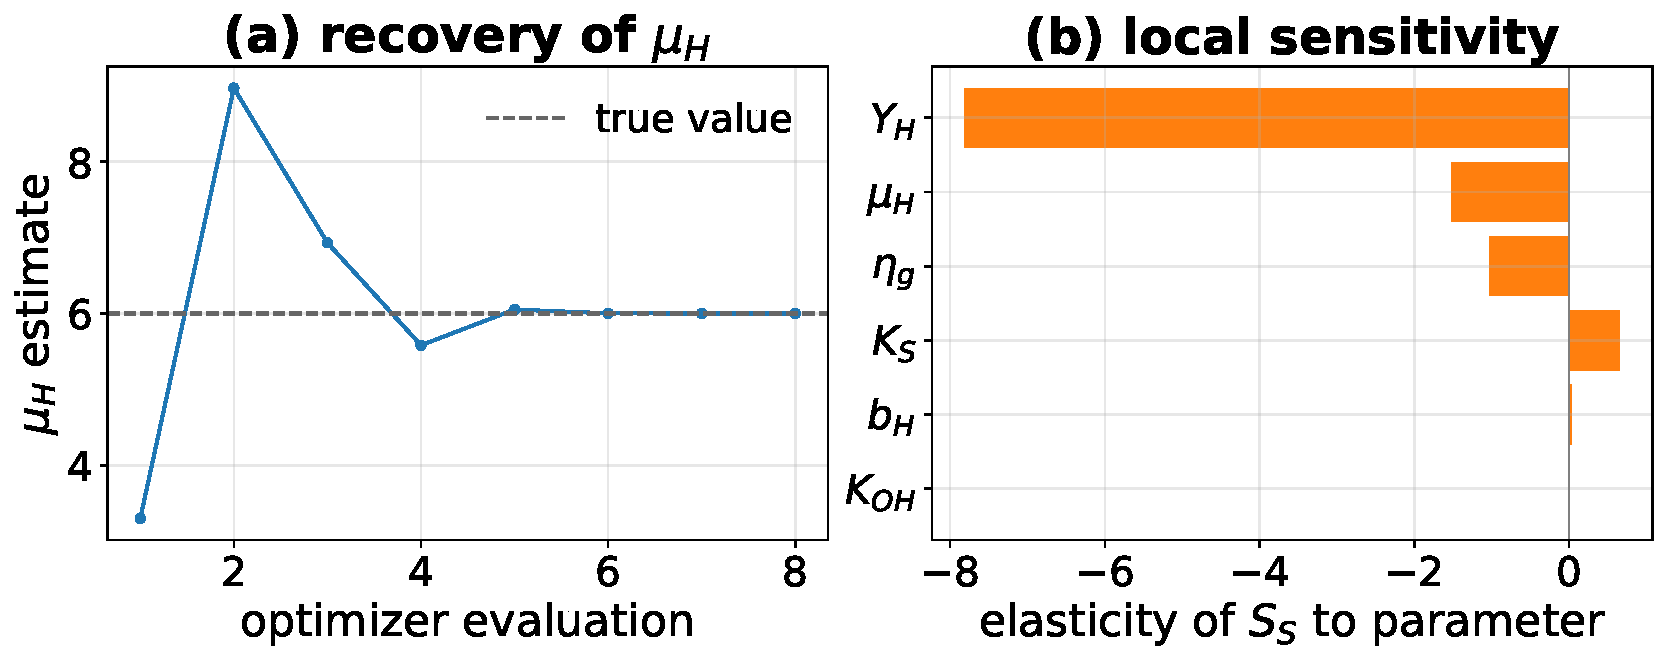
\includegraphics[width=0.72\linewidth]{fig_differentiability}
  \caption{Single-parameter, noise-free gradient-correctness check. (a) A
  gradient-based optimizer recovers the true \DiffParamName\ parameter of a single
  activated-sludge reactor from a perturbed start, using the exact reverse-mode
  gradient of the calibration objective. (b) The derivative-based local sensitivity
  of the observable to the kinetic parameters, normalized, from one forward-mode
  pass.}
  \label{fig:diff}
\end{figure}

\section{The discrete adjoint}
\label{si:discrete-adjoint}
The reverse-mode gradients used for calibration and for the plant are formed by a hand-written \emph{discrete adjoint} rather than by differentiating through the stiff solve. Reverse-mode differentiation \emph{through} an implicit solve stores each step's stage vector-field values \(\mathbf{f}_i\sim\lVert\mathbf{J}\rVert\,\mathbf{y}\), which are large for stiff modes, and forms cotangents of those large stored values, scaled by the step and compounded across stages and steps. Above a step-size threshold this overflows the floating-point range even though the true gradient is finite. The usual remedy limits the step size. The discrete adjoint removes that limitation by not differentiating through the solve at all.

For the implicit-Euler step \(\mathbf{y}_{n+1}=\mathbf{y}_n+\Delta t\,\mathbf{f}(\mathbf{y}_{n+1},\boldsymbol{\theta})\) the exact per-step sensitivities are
\[
\frac{\partial \mathbf{y}_{n+1}}{\partial \mathbf{y}_n}=(\mathbf{I}-\Delta t\,\mathbf{J})^{-1},\qquad \frac{\partial \mathbf{y}_{n+1}}{\partial\boldsymbol{\theta}}=\Delta t\,(\mathbf{I}-\Delta t\,\mathbf{J})^{-1} \mathbf{f}_{\boldsymbol{\theta}}, \qquad \mathbf{J}=\left.\frac{\partial \mathbf{f}}{\partial \mathbf{y}}\right|_{\mathbf{y}_{n+1}},
\]
so, with \(\ell\) the scalar loss and \(\bar{\mathbf{y}}_n=\partial\ell/\partial\mathbf{y}_n\) the cotangent of \(\mathbf{y}_n\), the reverse pass transposes these per-step sensitivities. Each backward step solves for the earlier-state cotangent,
\[
(\mathbf{I}-\Delta t\,\mathbf{J}^{\top})\,\bar{\mathbf{y}}_n=\bar{\mathbf{y}}_{n+1},
\]
and contributes one term to the parameter gradient, which over the whole trajectory is
\[
\frac{\partial\ell}{\partial\boldsymbol{\theta}}=\sum_{n}\Delta t\,\mathbf{f}_{\boldsymbol{\theta}}^{\top}\bar{\mathbf{y}}_n,
\]
with \(\mathbf{J}\) and \(\mathbf{f}_{\boldsymbol{\theta}}\) evaluated at \(\mathbf{y}_{n+1}\), and each observation's loss cotangent added to the state cotangent at its step. The recurrence has a direction, from the last step to the first; the sum does not, its order being immaterial. Every backward step is a single transposed solve through the same well-conditioned operator \(\mathbf{I}-\Delta t\,\mathbf{J}^{\top}\) the forward step used, a contraction, so the cotangent stays bounded and nothing overflows, at any step size. The model derivatives \(\mathbf{J}\) and \(\mathbf{f}_{\boldsymbol{\theta}}\) are taken by automatic differentiation of the rate function. Only the integrator's adjoint is written by hand. The high-order version used in practice replaces the single implicit stage with the transposed-stage recurrence of an \(s\)-stage ESDIRK method (the Kvaerno method the reactors use: \texttt{Kvaerno5} by default for a batch reactor, \texttt{Kvaerno3} for the plant), whose per-stage operators \(\mathbf{I}-\Delta t\,\gamma\,\mathbf{J}_i^{\top}\) are the transposes of the forward stage solves and whose stage values are reconstructed in the backward pass from the solver's saved stage increments rather than recomputed. This is the classical discrete-adjoint construction for implicit Runge--Kutta methods \citep{sandu2003, zhang2014}. The resulting gradient is the exact gradient of the discrete solve and is verified against the closed-form sensitivity of the stiff chain (Section~\ref{sec:results-verification-analytic}) and against a finite-difference gradient through the assembled plant (Section~\ref{sec:results-verification-fd}). These are the two regimes in which an independent reference is available. The stiff chain admits an analytic sensitivity but is small enough that differentiating through it is finite at any step, whereas the coupled plant is where differentiating through the solve overflows without a step-size limitation and no closed-form sensitivity exists. A further check is on single stiff units, where differentiating through the solve does stay finite, namely the activated-sludge batch and the anaerobic digester in isolation. There the discrete-adjoint gradient of a scalar loss, taken with respect to the full parameter vector, agrees with the through-solve gradient at every step-size cap tried, from \(\SIAdjBatchCapMin\)~d (batch) and \(\SIAdjDigCapMin\)~d (digester) up to no step-size limitation at all: to a relative difference of at most \SIAdjBatchRel\ on the batch at a solver tolerance of \(\SIAdjBatchRtol\), and \SIAdjDigRel\ on the digester at \(\SIAdjDigRtol\), confirming that the two compute the same derivative. The discrete adjoint's freedom from any step-size limitation is what lets the same gradient serve the coupled plant, where differentiating through the solve overflows without one and the discrete adjoint remains finite.

\section{Steady-state adjoint}
\label{si:steady-adjoint}
Section~\ref{sec:methods-ad} reduces the reverse-mode gradient of a steady-state output to the single transposed solve of Eq.~\eqref{eq:ift-adjoint}. This appendix derives that result from the implicit function theorem, shows why the transpose appears only in reverse mode, and explains why the solve costs little more than the root find that precedes it.

The steady state \(\mathbf{x}^\star(\boldsymbol{\theta})\) is defined implicitly as the root of the plant residual,
\[
\mathbf{F}\!\left(\mathbf{x}^\star(\boldsymbol{\theta}),\,\boldsymbol{\theta}\right)=\mathbf{0},
\]
and a scalar output, a calibration loss or any reported quantity, is \(\ell=\ell(\mathbf{x}^\star)\). The goal is \(\partial\ell/\partial\boldsymbol{\theta}\) without differentiating through the solver iteration.

\paragraph{The reverse-mode chain.} The output depends on the parameters through a chain of three links: the parameters set the residual \(\mathbf{F}\), the condition \(\mathbf{F}(\mathbf{x}^\star,\boldsymbol{\theta})=\mathbf{0}\) fixes the steady state, and the steady state sets the output,
\[
\boldsymbol{\theta}\;\longrightarrow\;\mathbf{x}^\star\;\longrightarrow\;\ell .
\]
Reverse-mode differentiation evaluates \(\partial\ell/\partial\boldsymbol{\theta}\) by traversing this chain backwards. At each stage it carries the derivative of the final scalar output with respect to the quantity at that stage; that derivative is a vector of the same shape as the quantity, and is called the quantity's \emph{cotangent}. The pass starts at the output itself, whose cotangent with respect to itself is \(1\), and differentiates the output function \(\ell(\mathbf{x}^\star)\) to obtain the cotangent of the state,
\[
\bar{\mathbf{x}}\equiv\left(\frac{\partial\ell}{\partial\mathbf{x}^\star}\right)^{\!\top},
\]
which is just the gradient of the output with respect to the state. Because the output is an ordinary explicit function, a loss or a reported quantity, \(\bar{\mathbf{x}}\) is obtained directly by running reverse mode once through it, at negligible cost and with no linear solve. The one link in the chain that is not an explicit formula is the middle one, the steady-state solve, because \(\mathbf{x}^\star\) is defined implicitly. The rest of this section explains how the cotangent is carried back across that link from \(\bar{\mathbf{x}}\), the cotangent of the state, to the cotangent of the parameters, which is the gradient being sought.

\paragraph{Implicit differentiation of the root.} The root identity holds for every \(\boldsymbol{\theta}\), so its total derivative with respect to \(\boldsymbol{\theta}\) vanishes. The two ways \(\boldsymbol{\theta}\) reaches \(\mathbf{F}\), directly and through \(\mathbf{x}^\star\), must cancel,
\[
\underbrace{\frac{\partial\mathbf{F}}{\partial\mathbf{x}}}_{\displaystyle \mathbf{J}}\,
\frac{\partial\mathbf{x}^\star}{\partial\boldsymbol{\theta}}
+\frac{\partial\mathbf{F}}{\partial\boldsymbol{\theta}}=\mathbf{0}
\qquad\Longrightarrow\qquad
\frac{\partial\mathbf{x}^\star}{\partial\boldsymbol{\theta}}
=-\mathbf{J}^{-1}\frac{\partial\mathbf{F}}{\partial\boldsymbol{\theta}},
\]
which is Eq.~\eqref{eq:ift}. The inverse exists on the operating branch, away from the folds where \(\mathbf{J}\) is singular and which the continuation of Section~\ref{sec:methods-steady} handles separately.

\paragraph{Chain rule to the output.} Combining this state sensitivity with the state cotangent \(\bar{\mathbf{x}}\) from the backward pass, again by the chain rule, gives the parameter gradient in closed form,
\begin{equation}
\frac{\partial\ell}{\partial\boldsymbol{\theta}}
=\frac{\partial\ell}{\partial\mathbf{x}^\star}\,\frac{\partial\mathbf{x}^\star}{\partial\boldsymbol{\theta}}
=-\,\bar{\mathbf{x}}^{\top}\mathbf{J}^{-1}\frac{\partial\mathbf{F}}{\partial\boldsymbol{\theta}}.
\label{eq:steady-grad-full}
\end{equation}
Everything here is known: \(\bar{\mathbf{x}}\) came from differentiating the output, \(\mathbf{J}\) and \(\partial\mathbf{F}/\partial\boldsymbol{\theta}\) from differentiating the residual. What remains is only the choice of the order in which to multiply them, and that choice is the whole story of the cost.

\paragraph{The order of multiplication is forward versus reverse mode.} Equation~\eqref{eq:steady-grad-full} is a product of three factors, the row vector \(\bar{\mathbf{x}}^{\top}\), the inverse \(\mathbf{J}^{-1}\), and the matrix \(\partial\mathbf{F}/\partial\boldsymbol{\theta}\). It can be multiplied out from the right or from the left, and the two orders give the same gradient at very different cost.
\emph{Forward mode} multiplies from the right, forming the sensitivity matrix first, \(\mathbf{Z}=-\mathbf{J}^{-1}\,\partial\mathbf{F}/\partial\boldsymbol{\theta}\). This means solving \(\mathbf{J}\,\mathbf{Z}=-\partial\mathbf{F}/\partial\boldsymbol{\theta}\) for one column of \(\mathbf{Z}\) per parameter, so \(n_p\) linear solves, and only then contracting with \(\bar{\mathbf{x}}\).
\emph{Reverse mode} multiplies from the left instead. Grouping the first two factors,
\[
\bar{\mathbf{x}}^{\top}\mathbf{J}^{-1}=\left(\mathbf{J}^{-\top}\bar{\mathbf{x}}\right)^{\top}\equiv\boldsymbol{\nu}^{\top}
\]
defines the adjoint \(\boldsymbol{\nu}\) as the solution of the single transposed system \(\mathbf{J}^{\top}\boldsymbol{\nu}=\bar{\mathbf{x}}\), after which
\[
\frac{\partial\ell}{\partial\boldsymbol{\theta}}=-\,\boldsymbol{\nu}^{\top}\frac{\partial\mathbf{F}}{\partial\boldsymbol{\theta}},
\]
which is Eq.~\eqref{eq:ift-adjoint}. The transpose is absent from Eq.~\eqref{eq:ift}; it appears only here, because reverse mode applies \(\mathbf{J}^{-1}\) to the \emph{left} of the cotangent, turning the forward solve against \(\mathbf{J}\) into a solve against \(\mathbf{J}^{\top}\). The remaining product \(\boldsymbol{\nu}^{\top}\,\partial\mathbf{F}/\partial\boldsymbol{\theta}\) is a vector--Jacobian product, taken by one reverse-mode pass through \(\mathbf{F}\) without ever assembling the matrix \(\partial\mathbf{F}/\partial\boldsymbol{\theta}\).

\paragraph{What the adjoint solves for.} The one quantity computed is the adjoint vector \(\boldsymbol{\nu}\), the same length as the state \(\mathbf{x}\), obtained from the single linear system \(\mathbf{J}^{\top}\boldsymbol{\nu}=\bar{\mathbf{x}}\); the gradient for every parameter then follows by the contraction \(-\boldsymbol{\nu}^{\top}\,\partial\mathbf{F}/\partial\boldsymbol{\theta}\), with no per-parameter solve. What \(\boldsymbol{\nu}\) represents makes this more than a regrouping. Perturb the steady-state equations by a small source, \(\mathbf{F}(\mathbf{x},\boldsymbol{\theta})=\mathbf{b}\): the root shifts by \(\delta\mathbf{x}=\mathbf{J}^{-1}\mathbf{b}\) and the output by \(\delta\ell=\bar{\mathbf{x}}^{\top}\mathbf{J}^{-1}\mathbf{b}=\boldsymbol{\nu}^{\top}\mathbf{b}\), so \(\boldsymbol{\nu}=\partial\ell/\partial\mathbf{b}\): its component \(\nu_i\) is the sensitivity of the output to a unit source added to the \(i\)-th steady-state equation. The adjoint equation \(\mathbf{J}^{\top}\boldsymbol{\nu}=\bar{\mathbf{x}}\) carries the output's state-sensitivity \(\bar{\mathbf{x}}\) back through the transposed steady-state operator to this residual-sensitivity. A parameter perturbs the residual by \(\partial\mathbf{F}/\partial\boldsymbol{\theta}\), which is exactly such a source, so its effect on the output is read straight off \(\boldsymbol{\nu}\). Equivalently \(\boldsymbol{\nu}\) is the Lagrange multiplier of the constraint \(\mathbf{F}=\mathbf{0}\): the stationarity of \(\ell(\mathbf{x})-\boldsymbol{\nu}^{\top}\mathbf{F}(\mathbf{x},\boldsymbol{\theta})\) in \(\mathbf{x}\) is the adjoint equation, and its derivative in \(\boldsymbol{\theta}\) is the gradient.

\paragraph{Cost and implementation.} Reverse mode returns the entire gradient in one transposed solve, independent of \(n_p\), whereas forward mode costs \(n_p\) linear solves; for calibration, many parameters against a scalar loss, this is the decisive difference. The engine forms \(\mathbf{J}=\partial\mathbf{F}/\partial\mathbf{x}\) once at the converged root by automatic differentiation, so the adjoint costs one Jacobian and one linear solve, with no per-parameter work. It registers the implicit-function tangent \(\delta\mathbf{x}=-\mathbf{J}^{-1}(\partial\mathbf{F}/\partial\boldsymbol{\theta})\,\delta\boldsymbol{\theta}\) as a custom forward-mode (JVP) rule of the steady-state solve. Because that map is linear in \(\delta\boldsymbol{\theta}\), JAX transposes it into the reverse-mode rule of Eq.~\eqref{eq:ift-adjoint}, so differentiation of a steady output in either mode uses the implicit function theorem rather than unrolling the iteration (Section~\ref{sec:methods-ad}).

\paragraph{Explicit parameter dependence and vector outputs.} If the output also depends on \(\boldsymbol{\theta}\) directly, \(\ell=\ell(\mathbf{x}^\star,\boldsymbol{\theta})\), the same steps give \(\partial\ell/\partial\boldsymbol{\theta}=\left.\partial\ell/\partial\boldsymbol{\theta}\right|_{\mathbf{x}^\star}-\boldsymbol{\nu}^{\top}\,\partial\mathbf{F}/\partial\boldsymbol{\theta}\) with the same adjoint \(\boldsymbol{\nu}\). For a vector output \(\mathbf{g}(\mathbf{x}^\star)\in\mathbb{R}^{m}\), reverse mode uses one transposed solve per output component and forward mode one per parameter, so the cheaper mode is set by \(\min(m,\,n_p)\); the scalar-loss case \(m=1\) is where the adjoint is most advantageous.

\end{document}
